\documentclass[12pt,a4paper]{article}
\usepackage[utf8]{inputenc}
\usepackage[T1]{fontenc}
\usepackage{lmodern,microtype,geometry,graphicx,booktabs,array,tabularx}
\usepackage{amsmath,amssymb,float,caption,subcaption,xcolor,hyperref,fancyhdr,tikz}
\usetikzlibrary{positioning,arrows.meta,calc}
\geometry{margin=1in}
\setlength{\headheight}{14.5pt}
\pagestyle{fancy}\fancyhf{}\lhead{Power Flow, Small-Signal Stability, and Time-Domain Simulation }\rhead{\thepage}
\hypersetup{colorlinks=true,linkcolor=blue,urlcolor=blue,citecolor=blue}
\renewcommand{\arraystretch}{1.12}
\captionsetup[table]{skip=7pt}
\title{\textbf{Padiyar Two-Area Four-Machine System}\\
\large Power Flow, Small-Signal Stability, and Time-Domain Simulation}
\date{13 July 2026}

\begin{document}
\maketitle

\begin{abstract}
This report reconstructs the four-machine, ten-bus, two-area system in
Padiyar, \emph{Power System Dynamics: Stability and Control}, second edition,
Section~9.6.1. Tables~9.1--9.4 are treated as the primary input source. Each
generator uses Padiyar model~1.1, a two-axis transient synchronous-machine
model, with either manual excitation or the printed single-time-constant AVR.
The AVR case has five states per generator and twenty states in total. The
in-house Newton--Raphson power flow, DAE equilibrium, small-signal
linearisation and implicit-trapezoidal time-domain simulation are generated from
project code. Table~9.5 is used only as a secondary published cross-check; no
parameter is fitted to its eigenvalues.
\end{abstract}
\newpage
\tableofcontents
\newpage

\section{Scope and source discipline}

The numerical inputs are transcribed from Padiyar Tables~9.1--9.4 (PDF
pages~338--344, printed pages~325--331). The source provides transient-axis
parameters $X'_d$, $X'_q$, $T'_{d0}$ and $T'_{q0}$, but no subtransient
parameters. Consequently, this report does not invent $X''$ or $T''$ data and
does not describe the model as sixth order. The two configurations are:

\begin{enumerate}
  \item \textbf{Manual excitation:} four machine states
  $[\delta,\omega,E'_q,E'_d]$ per generator, 16 states total.
  \item \textbf{Single-time-constant AVR:} the same machine plus $E_{fd}$,
  giving five states per generator and 20 states total.
\end{enumerate}

The cited pages do not provide a PSS design for this case. No PSS gain or time
constant is invented; a future PSS comparison requires a separately documented
design specification. This case replaces the former use of Kundur Table~E12.3
as the report reference.

\section{System description}

The network contains ten buses and four generators. Generators at buses 1 and
2 form Area~1, while generators at buses 11 and 12 form Area~2. Three parallel
circuits connect buses 3 and 13. The total connected active load is 2734~MW on
a 100-MVA base. Dynamic loads are represented as constant impedances, as
specified by Padiyar.

\begin{figure}[H]
\centering
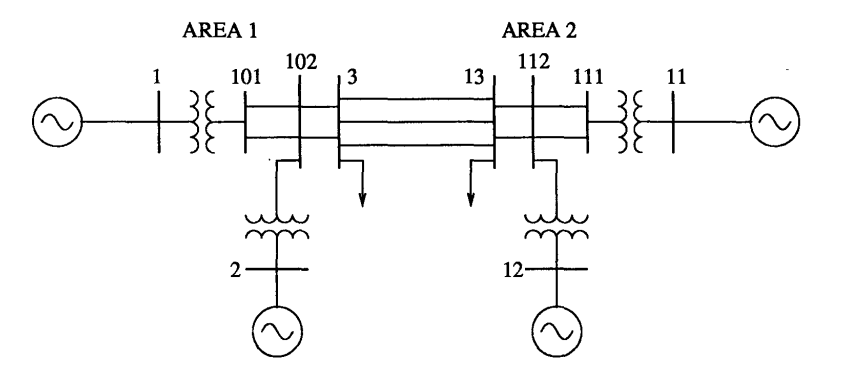
\includegraphics[width=\textwidth]{figures/padiyar_two_area/circuit_diagram.png}
\caption{Padiyar four-machine, ten-bus two-area network (source: Padiyar,
\emph{Power System Dynamics}, 2nd ed., Sec.~9.6.1). Generators at buses~1
and~2 form Area~1; generators at buses~11 and~12 form Area~2. Three parallel
circuits connect buses~3 and~13 across the inter-area tie. Loads are connected
at buses~3 and~13.}
\end{figure}

\section{Source data (Padiyar Tables 9.1--9.6)}

The following tables are transcribed verbatim from Padiyar, \emph{Power System
Dynamics: Stability and Control}, 2nd ed., Section~9.6.1 (printed
pages~325--331). They are the \emph{input} to the in-house computation; no value
below is a computed result. All quantities are on a 100-MVA base.

\begin{table}[H]\centering\scriptsize
\caption{Transmission line data on 100-MVA base (Padiyar Table~9.1).}
\begin{tabular}{ccccc}\toprule
From & To & $R_s$ (pu) & $X_s$ (pu) & $B$ (pu)\\\midrule
1 & 101 & 0.001 & 0.012 & 0.00\\
2 & 102 & 0.001 & 0.012 & 0.00\\
3 & 13  & 0.022 & 0.220 & 0.33\\
3 & 13  & 0.022 & 0.220 & 0.33\\
3 & 13  & 0.022 & 0.220 & 0.33\\
3 & 102 & 0.002 & 0.020 & 0.03\\
3 & 102 & 0.002 & 0.020 & 0.03\\
11 & 111 & 0.001 & 0.012 & 0.00\\
12 & 112 & 0.001 & 0.012 & 0.00\\
13 & 112 & 0.002 & 0.020 & 0.03\\
13 & 112 & 0.002 & 0.020 & 0.03\\
101 & 102 & 0.005 & 0.050 & 0.075\\
101 & 102 & 0.005 & 0.050 & 0.075\\
111 & 112 & 0.005 & 0.050 & 0.075\\
111 & 112 & 0.005 & 0.050 & 0.075\\\bottomrule
\end{tabular}\end{table}

\begin{table}[H]\centering\scriptsize
\caption{Load-flow data and results --- printed operating point (Padiyar Table~9.2).}
\begin{tabular}{cccccccc}\toprule
Bus & $|V|$ (pu) & $\theta$ (deg) & $P_G$ (pu) & $Q_G$ (pu) & $P_L$ (pu) & $Q_L$ (pu) & $B_{sh}$ (pu)\\\midrule
1   & 1.0300 & 8.2154   & 7.0     & 1.3386 & 0      & 0     & 0\\
2   & 1.0100 & -1.5040  & 7.0     & 1.5920 & 0      & 0     & 0\\
11  & 1.0300 & 0.0      & 7.2172  & 1.4466 & 0      & 0     & 0\\
12  & 1.0100 & -10.2051 & 7.0     & 1.8083 & 0      & 0     & 0\\
101 & 1.0108 & 3.6615   & 0       & 0      & 0      & 0     & 0\\
102 & 0.9875 & -6.2433  & 0       & 0      & 0      & 0     & 0\\
111 & 1.0095 & -4.6977  & 0       & 0      & 0      & 0     & 0\\
112 & 0.9850 & -14.9443 & 0       & 0      & 0      & 0     & 0\\
3   & 0.9761 & -14.4194 & 0       & 0      & 11.59  & 2.12  & 3.0\\
13  & 0.9716 & -23.2922 & 0       & 0      & 15.75  & 2.88  & 4.0\\\bottomrule
\end{tabular}\end{table}

\begin{table}[H]\centering\scriptsize
\caption{Machine data, identical for all four machines unless noted (Padiyar Table~9.3).}
\begin{tabular}{lcccc}\toprule
Variable & Bus 1 & Bus 2 & Bus 11 & Bus 12\\\midrule
$X_l$ (pu)        & 0.022   & 0.022   & 0.022   & 0.022\\
$R_a$ (pu)        & 0.00028 & 0.00028 & 0.00028 & 0.00028\\
$X_d$ (pu)        & 0.2     & 0.2     & 0.2     & 0.2\\
$X'_d$ (pu)       & 0.033   & 0.033   & 0.033   & 0.033\\
$T'_{d0}$ (s)     & 8.0     & 8.0     & 8.0     & 8.0\\
$X_q$ (pu)        & 0.19    & 0.19    & 0.19    & 0.19\\
$X'_q$ (pu)       & 0.061   & 0.061   & 0.061   & 0.061\\
$T'_{q0}$ (s)     & 0.4     & 0.4     & 0.4     & 0.4\\
$H$ (s)           & 54.0    & 54.0    & 63.0    & 63.0\\
$D$ (pu)          & 0       & 0       & 0       & 0\\\bottomrule
\end{tabular}\end{table}

\begin{table}[H]\centering
\caption{Excitation system data, single-time-constant AVR (Padiyar Table~9.4).}
\begin{tabular}{lcccc}\toprule
Variable & Bus 1 & Bus 2 & Bus 11 & Bus 12\\\midrule
$K_A$ (pu)  & 200  & 200  & 200  & 200\\
$T_A$ (s)   & 0.02 & 0.02 & 0.02 & 0.02\\\bottomrule
\end{tabular}\end{table}


\begin{table}[H]\centering\scriptsize
\caption{Participation factors of the swing modes (Padiyar Table~9.6).
($\omega_1=7.29$, $\omega_2=6.69$, $\omega_3=4.44$ rad/s).}
\begin{tabular}{cccc}\toprule
Variable & Mode \#1 & Mode \#2 & Mode \#3\\\midrule
$\Delta S_{m1}$ (bus 1)  & $-0.18 \pm j0.14$  & $0.004 \pm j0.001$ & $-0.06 \pm j0.15$\\
$\Delta S_{m2}$ (bus 2)  & $-0.27 \pm j0.14$  & $0.00 \pm j0.00$   & $-0.062 \pm j0.07$\\
$\Delta S_{m3}$ (bus 11) & $-0.00 \pm j0.00$  & $0.24 \pm j0.03$   & $-0.068 \pm j0.13$\\
$\Delta S_{m4}$ (bus 12) & $-0.04 \pm j0.00$  & $0.30 \pm j0.08$   & $-0.061 \pm j0.07$\\\bottomrule
\end{tabular}\end{table}

The inter-area mode (mode~3, $\omega\approx4.44$~rad/s) has comparable
participation from all four machines, confirming its inter-area character.
Modes~1 and~2 are local to Area~1 and Area~2 respectively.


\section{Power-flow analysis}

The project-owned Newton--Raphson solver uses bus~11 as the reference bus,
matching the zero angle printed in Table~9.2. Buses 1, 2 and 12 are PV buses.
Line susceptance $B$ from Table~9.1 is represented as $B/2$ at each end of the
standard $\pi$ model. This convention reproduces the printed operating point.

\subsection{Newton--Raphson formulation}

The solver iterates on the polar voltage state $x=[\theta_2,\ldots,\theta_N,\,
|V|_{PQ_1},\ldots]^T$ (slack angle fixed, PV magnitudes fixed). Bus power
injections are computed from the admittance matrix $Y=G+jB$:
\begin{align}
P_i(x) &= |V_i|\sum_{j=1}^{N}|V_j|\bigl(G_{ij}\cos\theta_{ij}+B_{ij}\sin\theta_{ij}\bigr),\\
Q_i(x) &= |V_i|\sum_{j=1}^{N}|V_j|\bigl(G_{ij}\sin\theta_{ij}-B_{ij}\cos\theta_{ij}\bigr),
\end{align}
where $\theta_{ij}=\theta_i-\theta_j$. The power mismatch is
$\Delta P_i=P_i^{\text{spec}}-P_i(x)$, $\Delta Q_i=Q_i^{\text{spec}}-Q_i(x)$.
At each iteration the Newton step solves
\begin{equation}
J(x_k)\,\Delta x = \begin{bmatrix}\Delta P\\ \Delta Q\end{bmatrix},
\qquad x_{k+1}=x_k+\Delta x,
\end{equation}
where $J$ is the standard $4$-block Jacobian with sub-matrices
$H=\partial P/\partial\theta$, $N=\partial P/\partial|V|$,
$M=\partial Q/\partial\theta$, $L=\partial Q/\partial|V|$. Iteration
terminates when $\max|\Delta P,\Delta Q|<10^{-10}$. No external nonlinear
solver is used; the Jacobian is built analytically from~$Y$ in project code.


\begin{table}[H]\centering
\caption{Power-flow convergence and Table~9.2 comparison.}
\begin{tabular}{@{}lr@{}}\toprule Quantity & Value\\ \midrule
Converged & Yes\\
Iterations & 3\\
Maximum $|\Delta V|$ vs Table 9.2 & 4.927e-05 pu\\
Maximum $|\Delta \theta|$ vs Table 9.2 & 4.983e-05 deg\\
Total generation & 2821.72 MW\\
Total load & 2734.00 MW\\
Total loss & 87.72 MW\\
\bottomrule\end{tabular}

\end{table}

\begin{table}[H]\centering\small
\caption{Power-flow comparison: Padiyar Table~9.2 versus the in-house
solution. Absolute differences are reported because an angle percentage error
is undefined at the zero-angle reference bus.}
\resizebox{\textwidth}{!}{\begin{tabular}{rrrrrrr}\toprule
{Bus} & {$V_{book}$} & {$V_{ours}$} & {$|\Delta V|$} & {$\theta_{book}$} & {$\theta_{ours}$} & {$|\Delta\theta|$}\\
{} & {(pu)} & {(pu)} & {(pu)} & {(deg)} & {(deg)} & {(deg)}\\ \midrule
1 & 1.0300 & 1.0300 & 0.00e+00 & 8.2154 & 8.2154 & 4.98e-05\\
2 & 1.0100 & 1.0100 & 0.00e+00 & -1.5040 & -1.5040 & 1.13e-05\\
11 & 1.0300 & 1.0300 & 0.00e+00 & 0.0000 & 0.0000 & 0.00e+00\\
12 & 1.0100 & 1.0100 & 0.00e+00 & -10.2051 & -10.2051 & 6.79e-06\\
101 & 1.0108 & 1.0108 & 5.72e-07 & 3.6615 & 3.6615 & 1.83e-05\\
102 & 0.9875 & 0.9875 & 3.06e-05 & -6.2433 & -6.2433 & 2.33e-05\\
111 & 1.0095 & 1.0095 & 3.02e-05 & -4.6977 & -4.6977 & 3.44e-05\\
112 & 0.9850 & 0.9850 & 4.83e-05 & -14.9443 & -14.9443 & 4.15e-05\\
3 & 0.9761 & 0.9761 & 1.43e-05 & -14.4194 & -14.4194 & 3.67e-05\\
13 & 0.9716 & 0.9716 & 4.93e-05 & -23.2922 & -23.2922 & 1.74e-05\\
\bottomrule\end{tabular}
}
\end{table}

\begin{table}[H]\centering\small
\caption{Detailed in-house power-flow results (mirrors the launcher output).
All powers are in pu on the 100-MVA base.}
\resizebox{\textwidth}{!}{\begin{tabular}{rlrrrrrrrr}\toprule
{Bus} & {Type} & {$|V|$} & {$\theta$} & {$P_G$} & {$Q_G$} & {$P_L$} & {$Q_L$} & {$P_{net}$} & {$Q_{net}$}\\
{} & {} & {(pu)} & {(deg)} & {(pu)} & {(pu)} & {(pu)} & {(pu)} & {(pu)} & {(pu)}\\ \midrule
1 & PV & 1.0300 & 8.2154 & 7.0000 & 1.3386 & 0.0000 & 0.0000 & 7.0000 & 1.3386\\
2 & PV & 1.0100 & -1.5040 & 7.0000 & 1.5920 & 0.0000 & 0.0000 & 7.0000 & 1.5920\\
11 & REF & 1.0300 & 0.0000 & 7.2172 & 1.4466 & 0.0000 & 0.0000 & 7.2172 & 1.4466\\
12 & PV & 1.0100 & -10.2051 & 7.0000 & 1.8083 & 0.0000 & 0.0000 & 7.0000 & 1.8083\\
101 & PQ & 1.0108 & 3.6615 & 0.0000 & 0.0000 & 0.0000 & 0.0000 & 0.0000 & 0.0000\\
102 & PQ & 0.9875 & -6.2433 & 0.0000 & 0.0000 & 0.0000 & 0.0000 & 0.0000 & 0.0000\\
111 & PQ & 1.0095 & -4.6977 & 0.0000 & 0.0000 & 0.0000 & 0.0000 & 0.0000 & 0.0000\\
112 & PQ & 0.9850 & -14.9443 & 0.0000 & 0.0000 & 0.0000 & 0.0000 & 0.0000 & 0.0000\\
3 & PQ & 0.9761 & -14.4194 & 0.0000 & 0.0000 & 11.5900 & 2.1200 & -11.5900 & -2.1200\\
13 & PQ & 0.9716 & -23.2922 & 0.0000 & 0.0000 & 15.7500 & 2.8800 & -15.7500 & -2.8800\\
\bottomrule\end{tabular}
}
\end{table}

\begin{figure}[H]\centering
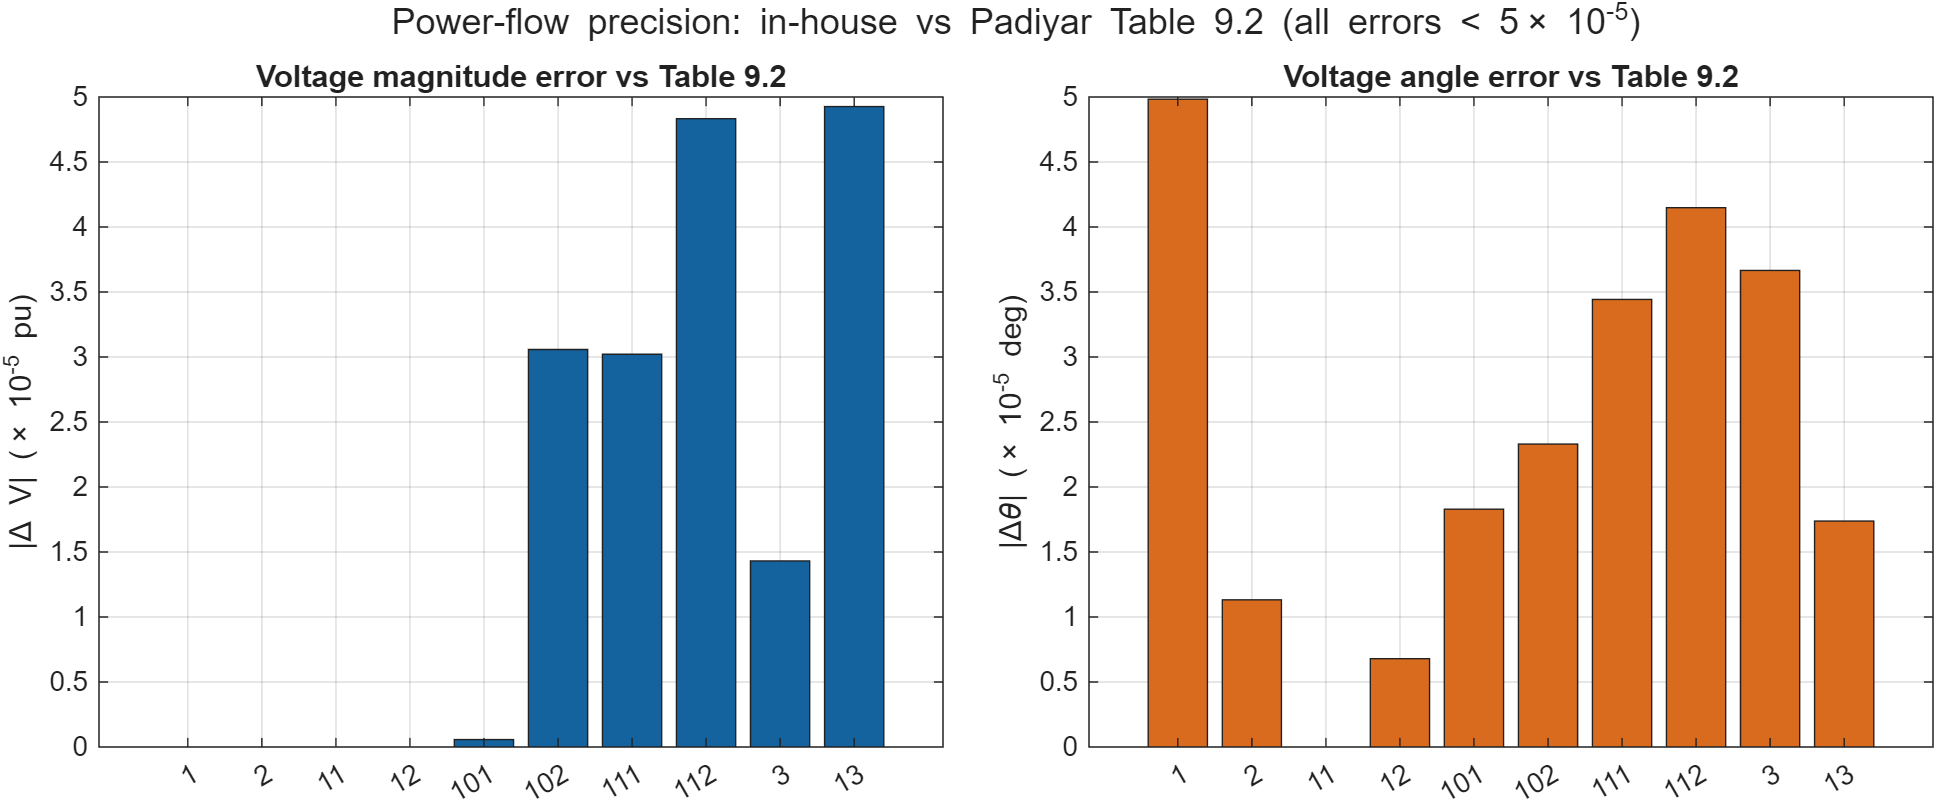
\includegraphics[width=\textwidth]{figures/padiyar_two_area/pf_precision.png}
\caption{Power-flow precision: in-house values versus Padiyar Table~9.2.
Top row---voltage-magnitude and angle scatter with the 1:1 diagonal (points on
the line indicate exact agreement). Bottom row---per-bus absolute errors
$|\Delta V|$ and $|\Delta\theta|$, all below $5\times10^{-5}$.}
\end{figure}

\begin{figure}[H]\centering

\includegraphics[width=\textwidth]{figures/padiyar_two_area/powerflow_summary.png}
\caption{In-house power-flow result and Newton--Raphson convergence.}
\end{figure}

\section{Model 1.1 with AVR}

For generator $i$, the state order and its corresponding derivative order are
\begin{equation}
x_i=\bigl[\delta_i,\ \omega_i,\ E'_{qi},\ E'_{di},\ E_{fdi}\bigr]^T,
\qquad
\dot{x}_i=\bigl[\dot\delta_i,\ \dot\omega_i,\
\dot E'_{qi},\ \dot E'_{di},\ \dot E_{fdi}\bigr]^T
=f_i(x_i,I_{di},I_{qi},|V_i|,u_i),
\end{equation}
where the overdot denotes the time derivative. The complete input-driven DAE is
\begin{equation}
\dot x=f(x,y,u),\qquad 0=g(x,y,u),
\label{eq:input-dae}
\end{equation}
where
\begin{equation}
\begin{aligned}
y&=\begin{bmatrix}\Re(V)^T&\Im(V)^T\end{bmatrix}^{T},\qquad
u=\begin{bmatrix}P_m^T&u_{exc}^{T}&\rho\end{bmatrix}^{T},\\
u_{exc}&=
\begin{cases}V_{ref},&\text{AVR},\\E_{fd0},&\text{manual excitation}.
\end{cases}
\end{aligned}
\label{eq:xyu-order}
\end{equation}
Thus $x$ contains differential machine/AVR states, $y$ contains algebraic bus
voltages, and $u$ contains prescribed inputs: mechanical power $P_m$,
excitation command $u_{exc}$, and topology selector $\rho$. Equilibrium and SSSA hold
$u=u_0$ fixed; TS changes only $\rho(t)$ at the declared event times.
Generator current is positive from the machine into the network. The dynamic
equations implemented in the shared DAE are
\begin{align}
\dot\delta_i &= \omega_B(\omega_i-1),\\
2H_i\dot\omega_i &= P_{mi}-P_{ei}-D_i(\omega_i-1),\\
T'_{d0i}\dot E'_{qi} &= E_{fdi}-E'_{qi}-(X_{di}-X'_{di})I_{di},\\
T'_{q0i}\dot E'_{di} &= -E'_{di}+(X_{qi}-X'_{qi})I_{qi},\\
T_{Ai}\dot E_{fdi} &= K_{Ai}(V_{ref,i}-|V_i|)-E_{fdi}.
\end{align}
The transient-saliency stator interface is
\begin{align}
V_{di}&=E'_{di}-R_aI_{di}+X'_qI_{qi},\\
V_{qi}&=E'_{qi}-R_aI_{qi}-X'_dI_{di}.
\end{align}
Air-gap electrical power is calculated directly as
\begin{equation}
P_{ei}=V_{di}I_{di}+V_{qi}I_{qi}+R_a(I_{di}^2+I_{qi}^2).
\end{equation}
The same nonlinear functions are used for equilibrium, SSSA and TS.

\subsection{AVR versus manual excitation}

Two excitation configurations are studied from the same DAE:
\begin{itemize}
  \item \textbf{With AVR (5 states/machine, 20 total).} The field voltage
  $E_{fd}$ is a dynamic state governed by the single-time-constant AVR of
  Table~9.4 ($K_A=200$, $T_A=0.02$~s):
  \begin{equation}
  T_A\dot E_{fd}=K_A(V_{ref}-|V|)-E_{fd}.
  \label{eq:avr-time}
  \end{equation}
  At equilibrium $\dot E_{fd}=0$; therefore the voltage error is not zero but
  is exactly the field voltage divided by the gain:
  \begin{equation}
  E_{fd0}=K_A(V_{ref}-|V_0|),\qquad
  V_{ref}=|V_0|+\frac{E_{fd0}}{K_A}.
  \label{eq:avr-equilibrium}
  \end{equation}
  Linearising \eqref{eq:avr-time} with $\Delta V_{ref}=0$ gives
  \begin{equation}
  \Delta E_{fd}(s)=-\frac{K_A}{1+sT_A}\Delta|V|(s).
  \label{eq:avr-transfer}
  \end{equation}
  Hence $\Delta|V|<0$ produces $\Delta E_{fd}>0$. The DC correction gain is
  200 and the AVR pole is $-1/T_A=-50~\mathrm{s}^{-1}$, mathematically
  explaining its fast voltage-support action. This is the
  \emph{configuration published in the book}: Table~9.5 lists exactly 20
  eigenvalues, matching the $4\times5=20$ state count. The inter-area swing
  mode is nevertheless very lightly damped. For
  $\lambda=\sigma+j\omega_d$,
  \begin{equation}
  \zeta=-\frac{\sigma}{\sqrt{\sigma^2+\omega_d^2}}.
  \label{eq:damping-ratio}
  \end{equation}
  The computed AVR pole $-0.0042+j4.4565$ therefore gives
  \begin{equation}
  \zeta_{AVR}=\frac{0.0042}{\sqrt{0.0042^2+4.4565^2}}
  =9.5\times10^{-4}=0.095\%.
  \end{equation}
  The lightly damped conclusion thus follows from the computed pole.
  \item \textbf{Manual excitation/no AVR (4 states/machine, 16 total).}
  Removing the AVR does not remove the generator field circuit. Instead, the
  operator-supplied field voltage is frozen at the equilibrium value:
  \begin{equation}
  E_{fd}(t)=E_{fd0},\qquad \Delta E_{fd}(s)=0.
  \label{eq:manual-field}
  \end{equation}
  The manual state and input orders are therefore
  \begin{equation}
  x_i^{manual}=
  \begin{bmatrix}\delta_i&\omega_i&E'_{qi}&E'_{di}\end{bmatrix}^{T},
  \qquad
  u_i^{manual}=
  \begin{bmatrix}P_{mi}&E_{fd0,i}&\rho\end{bmatrix}^{T}.
  \label{eq:manual-state-input}
  \end{equation}
  The four retained differential equations are
  \begin{align}
  \dot\delta_i&=\omega_B(\omega_i-1),\\
  \dot\omega_i&=
  \frac{P_{mi}-P_{ei}-D_i(\omega_i-1)}{2H_i},\\
  \dot E'_{qi}&=
  \frac{E_{fd0,i}-E'_{qi}-(X_{di}-X'_{di})I_{di}}{T'_{d0i}},\\
  \dot E'_{di}&=
  \frac{-E'_{di}+(X_{qi}-X'_{qi})I_{qi}}{T'_{q0i}}.
  \label{eq:manual-dynamics}
  \end{align}
  Thus manual excitation still has rotor, speed, $d$-axis flux, $q$-axis
  flux, stator-current, and network-voltage dynamics. What disappears is only
  the closed-loop field-voltage state and its terminal-voltage feedback.

  Linearising the third equation in \eqref{eq:manual-dynamics} gives
  \begin{equation}
  \Delta\dot E'_q=
  -\frac{1}{T'_{d0}}\Delta E'_q
  -\frac{X_d-X'_d}{T'_{d0}}\Delta I_d
  +\frac{1}{T'_{d0}}\underbrace{\Delta E_{fd}}_{0}.
  \label{eq:manual-linear-field}
  \end{equation}
  Compare this with the AVR perturbation obtained from
  \eqref{eq:avr-time}:
  \begin{equation}
  \Delta\dot E_{fd}
  =-\frac{1}{T_A}\Delta E_{fd}
   -\frac{K_A}{T_A}\Delta|V|
   +\frac{K_A}{T_A}\Delta V_{ref}.
  \label{eq:avr-linear-field}
  \end{equation}
  With $\Delta V_{ref}=0$, the AVR introduces the coupling
  $-(K_A/T_A)\Delta|V|$ and one additional state. Manual excitation has
  neither term. In state-matrix form this means
  \begin{equation}
  \begin{aligned}
  \Delta\dot x_{manual}&=A_{manual}\Delta x_{manual},
  &A_{manual}&\in\mathbb{R}^{16\times16},\\
  \Delta\dot x_{AVR}&=A_{AVR}\Delta x_{AVR},
  &A_{AVR}&\in\mathbb{R}^{20\times20}.
  \end{aligned}
  \end{equation}
  No-AVR also does not mean constant terminal voltage: $V$ remains an
  algebraic solution of $g(x,y,u)=0$ and changes whenever machine current or
  network topology changes. Only $E_{fd}$ is constant.

  This manual case is a separate 16-state study; it does \emph{not} reproduce
  the 20-state Table~9.5. Its computed inter-area pole
  $-0.1173+j4.0712$ gives
  \begin{equation}
  \zeta_{manual}=\frac{0.1173}{\sqrt{0.1173^2+4.0712^2}}
  =0.0288=2.88\%.
  \end{equation}
  The comparison is consequently equation-based: the AVR improves voltage
  regulation through \eqref{eq:avr-transfer}, while adding the feedback block
  \eqref{eq:avr-linear-field} changes the full system matrix and moves this
  inter-area pole from $\zeta=2.88\%$ to $\zeta=0.095\%$. This observation
  applies to the stated operating point and printed AVR parameters; it is not
  a universal claim that every AVR reduces damping.
\end{itemize}
The book uses the AVR throughout Section~9.6.1: Table~9.4 supplies the AVR
parameters and Table~9.5 reports the 20-state eigenvalue spectrum. The manual
case is a project-defined comparison, not a book configuration.

\section{Small-signal stability}

The complete DAE is linearised numerically around the in-house power-flow
operating point. Algebraic network-voltage perturbations are eliminated with a
Schur complement. The published eigenvalues are transcribed in
the table below (Source data); they are not copied into the computed
column and are not used to tune parameters.

\subsection{Linearisation and Schur reduction}

The nonlinear DAE in \eqref{eq:input-dae} is linearised about
$(x_0,y_0,u_0)$ after verifying
\begin{equation}
\|f(x_0,y_0,u_0)\|_\infty\le\varepsilon_{eq},\qquad
\|g(x_0,y_0,u_0)\|_\infty\le\varepsilon_{eq}.
\end{equation}
SSSA fixes the external input, $\Delta u=0$. Substituting
$x=x_0+\Delta x$ and $y=y_0+\Delta y$ and retaining first-order terms gives
\begin{equation}
\begin{bmatrix}\Delta\dot x\\0\end{bmatrix}
=
\begin{bmatrix}J_{xx}&J_{xy}\\J_{yx}&J_{yy}\end{bmatrix}
\begin{bmatrix}\Delta x\\\Delta y\end{bmatrix}.
\label{eq:sssa-linear-dae}
\end{equation}
The Jacobian blocks are
\begin{equation}
J_{xx}=\tfrac{\partial f}{\partial x},\quad
J_{xy}=\tfrac{\partial f}{\partial y},\quad
J_{yx}=\tfrac{\partial g}{\partial x},\quad
J_{yy}=\tfrac{\partial g}{\partial y}.
\end{equation}
They are evaluated by central differences. For example,
\begin{align}
J_{xx}(:,k)&\approx
\frac{f(x_0+h e_k,y_0,u_0)-f(x_0-h e_k,y_0,u_0)}{2h},\\
J_{yx}(:,k)&\approx
\frac{g(x_0+h e_k,y_0,u_0)-g(x_0-h e_k,y_0,u_0)}{2h},
\end{align}
with $h=10^{-6}$; $J_{xy}$ and $J_{yy}$ use $y_0\pm h e_k$. These are
derivatives of the DAE equations, not derivatives of the reference table.

The algebraic row is solved as
\begin{equation}
J_{yy}\Delta y=-J_{yx}\Delta x.
\end{equation}
The code computes $K=J_{yy}\backslash J_{yx}$, avoiding an explicit inverse,
and substitutes $\Delta y=-K\Delta x$ into the differential row:
\begin{equation}
A=J_{xx}-J_{xy}K
=J_{xx}-J_{xy}J_{yy}^{-1}J_{yx},\qquad
\Delta\dot x=A\Delta x.
\label{eq:sssa-schur}
\end{equation}

\subsection{Eigenvalue solution and modal quantities}

The solver then evaluates
\begin{equation}
A v_i=\lambda_i v_i,\qquad
\det(\lambda_iI-A)=0,qquad \lambda_i=\sigma_i+j\omega_{d,i}.
\end{equation}
For each conjugate pair,
\begin{equation}
f_i=\frac{|\omega_{d,i}|}{2\pi},\qquad
\zeta_i=-\frac{\sigma_i}{\sqrt{\sigma_i^2+\omega_{d,i}^2}},\qquad
\tau_i=-\frac{1}{\sigma_i}\quad(\sigma_i<0).
\label{eq:sssa-modal-metrics}
\end{equation}
A physical mode is asymptotically stable when $\sigma_i<0$. Table~9 uses the
full 20-state AVR matrix, matching the original-matrix column of Padiyar
Table~9.5. The optional COI reduction is explicitly disabled in this execution,
so the rotational reference-angle mode remains near the origin and is not
misclassified as an unstable physical mode. Table~10 selects the
positive-imaginary roots with $1<\omega_d<10$ rad/s; the omitted conjugates
have identical $f$ and $\zeta$.

Reference matching occurs only after \eqref{eq:sssa-schur} has been solved.
One-to-one assignment minimizes $|\lambda_{ours}-\lambda_{book}|$ without
changing $A$ or a model parameter. The reported errors are
\begin{equation}
\varepsilon_\lambda=
100\frac{|\lambda_{ours}-\lambda_{book}|}{|\lambda_{book}|},\quad
\varepsilon_f=100\frac{|f_{ours}-f_{book}|}{f_{book}},\quad
\varepsilon_\zeta=
100\frac{|\zeta_{ours}-\zeta_{book}|}{|\zeta_{book}|}.
\end{equation}
The eigenvalue percentage is omitted for the near-zero reference pair because
its denominator makes a relative error numerically meaningless.

\begin{table}[H]\centering\small
\caption{Eigenvalue comparison: book values ($\lambda_{book}$, Padiyar
Table~9.5) versus in-house computed values ($\lambda_{ours}$), with absolute
difference $|\Delta\lambda|$ and swing-mode labels. Percentage error is
omitted for near-zero reference-angle modes because it is not numerically
meaningful. All 18 non-reference modes are stable.}




\resizebox{\textwidth}{!}{\begin{tabular}{rccrcl}\toprule
{No.} & {$\lambda_{book}$} & {$\lambda_{ours}$} & {$|\Delta\lambda|$} & {$\varepsilon_{\lambda}$} & {Mode}\\
{} & {(s$^{-1}$)} & {(s$^{-1}$)} & {(s$^{-1}$)} & {(\%)} & {}\\ \midrule
1 & $-39.9893$ & $-40.0225$ & 0.0332 & {0.08} & \\
2 & $-39.4922$ & $-39.5270$ & 0.0348 & {0.09} & \\
3 & $-24.5058 +20.6749j$ & $-24.5061 +20.6319j$ & 0.0430 & {0.13} & \\
4 & $-24.5058 -20.6749j$ & $-24.5061 -20.6319j$ & 0.0430 & {0.13} & \\
5 & $-25.0383 +11.9973j$ & $-25.0384 +11.9598j$ & 0.0375 & {0.13} & \\
6 & $-25.0383 -11.9973j$ & $-25.0384 -11.9598j$ & 0.0375 & {0.13} & \\
7 & $-11.5835$ & $-11.5566$ & 0.0269 & {0.23} & \\
8 & $-11.1735$ & $-11.1485$ & 0.0250 & {0.22} & \\
9 & $-0.7594 +7.2938j$ & $-0.7553 +7.3157j$ & 0.0223 & {0.30} & Swing 1\\
10 & $-0.7594 -7.2938j$ & $-0.7553 -7.3157j$ & 0.0223 & {0.30} & Swing 1\\
11 & $-0.7365 +6.6899j$ & $-0.7336 +6.7108j$ & 0.0211 & {0.31} & Swing 2\\
12 & $-0.7365 -6.6899j$ & $-0.7336 -6.7108j$ & 0.0211 & {0.31} & Swing 2\\
13 & $-0.0044 +4.4444j$ & $-0.0042 +4.4565j$ & 0.0121 & {0.27} & Inter-area\\
14 & $-0.0044 -4.4444j$ & $-0.0042 -4.4565j$ & 0.0121 & {0.27} & Inter-area\\
15 & $-4.5727$ & $-4.5701$ & 0.0026 & {0.06} & \\
16 & $-4.4802$ & $-4.4776$ & 0.0026 & {0.06} & \\
17 & $-4.1121$ & $-4.1095$ & 0.0026 & {0.06} & \\
18 & $0.0000 +0.0017j$ & $0.0000 +0.0000j$ & 0.0017 & {--} & \\
19 & $0.0000 -0.0017j$ & $0.0000 -0.0000j$ & 0.0017 & {--} & \\
20 & $-4.2449$ & $-4.2423$ & 0.0026 & {0.06} & \\
\bottomrule\end{tabular}
}
\end{table}

\begin{figure}[H]\centering
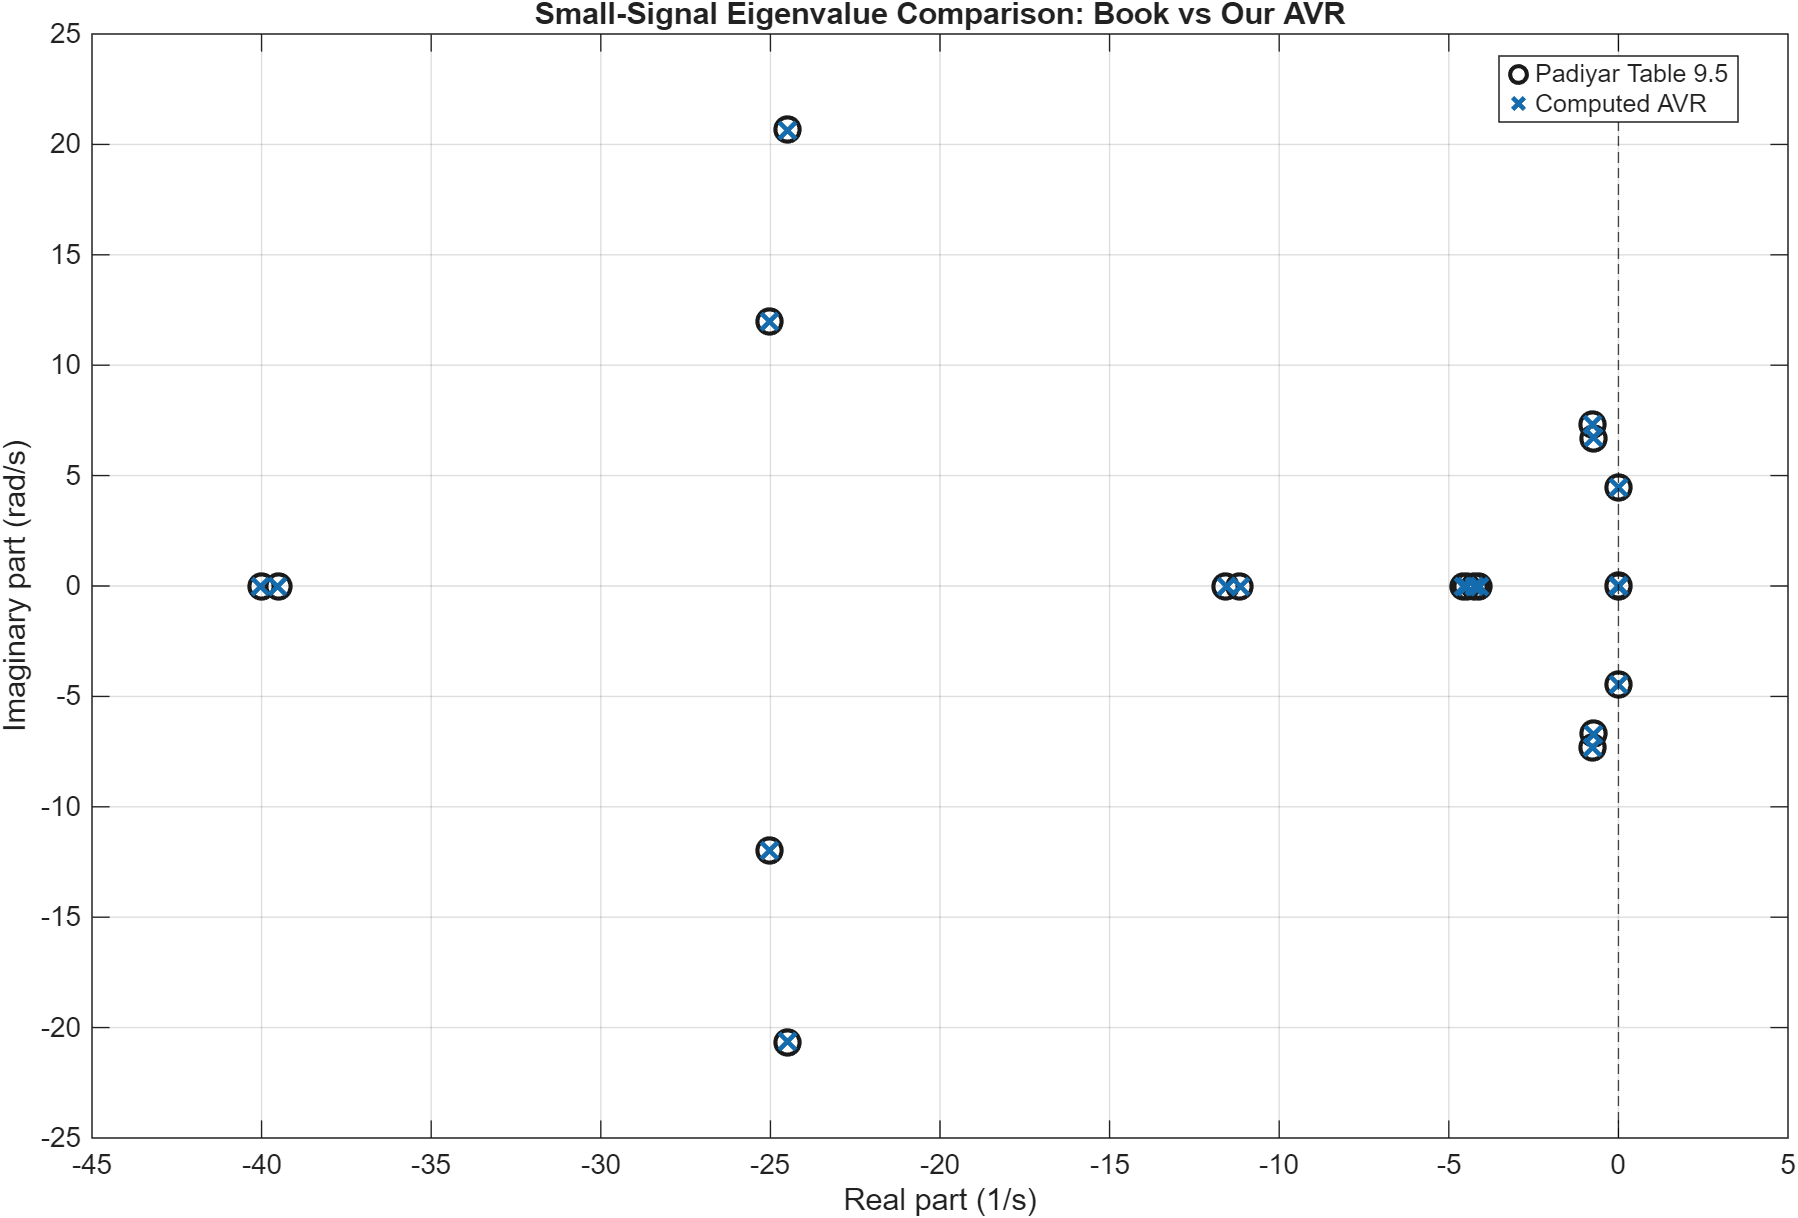
\includegraphics[width=.92\textwidth]{figures/padiyar_two_area/eigenvalue_comparison.png}
\caption{Graphical counterpart of Table~9 using only the AVR comparison on
one complex-plane axis. Independently transcribed Padiyar Table~9.5 values
are circles and computed AVR eigenvalues are crosses; coincident markers show
direct graphical agreement.}
\end{figure}

\begin{table}[H]\centering
\caption{SSSA swing-mode comparison. Each AVR row directly compares the
published and in-house eigenvalue, frequency, and damping ratio. Manual
excitation has no published counterpart because it has a different state
count; unavailable reference cells are shown with dashes. Both frequency and
damping-ratio percentage errors are calculated directly from the displayed
values.}
\resizebox{\textwidth}{!}{\begin{tabular}{llccrrrrrr}\toprule
{Configuration} & {Mode} & {$\lambda_{book}$} & {$\lambda_{ours}$} & {$f_{book}$} & {$f_{ours}$} & {$\varepsilon_f$} & {$\zeta_{book}$} & {$\zeta_{ours}$} & {$\varepsilon_{\zeta}$}\\
{} & {} & {(s$^{-1}$)} & {(s$^{-1}$)} & {(Hz)} & {(Hz)} & {(\%)} & {(\%)} & {(\%)} & {(\%)}\\ \midrule
AVR & Inter-area & $-0.0044+4.4444j$ & $-0.0042+4.4565j$ & 0.7073 & 0.7093 & 0.27 & 0.099 & 0.095 & 3.79\\
AVR & Local Area 2 & $-0.7365+6.6899j$ & $-0.7336+6.7108j$ & 1.0647 & 1.0680 & 0.31 & 10.943 & 10.867 & 0.70\\
AVR & Local Area 1 & $-0.7594+7.2938j$ & $-0.7553+7.3157j$ & 1.1608 & 1.1643 & 0.30 & 10.356 & 10.269 & 0.83\\
Manual & Inter-area & {--} & $-0.1173+4.0712j$ & {--} & 0.6480 & {--} & {--} & 2.880 & {--}\\
Manual & Local Area 2 & {--} & $-0.4296+6.6775j$ & {--} & 1.0627 & {--} & {--} & 6.420 & {--}\\
Manual & Local Area 1 & {--} & $-0.4460+7.2336j$ & {--} & 1.1513 & {--} & {--} & 6.154 & {--}\\
\bottomrule\end{tabular}
}
\end{table}

\begin{figure}[H]\centering
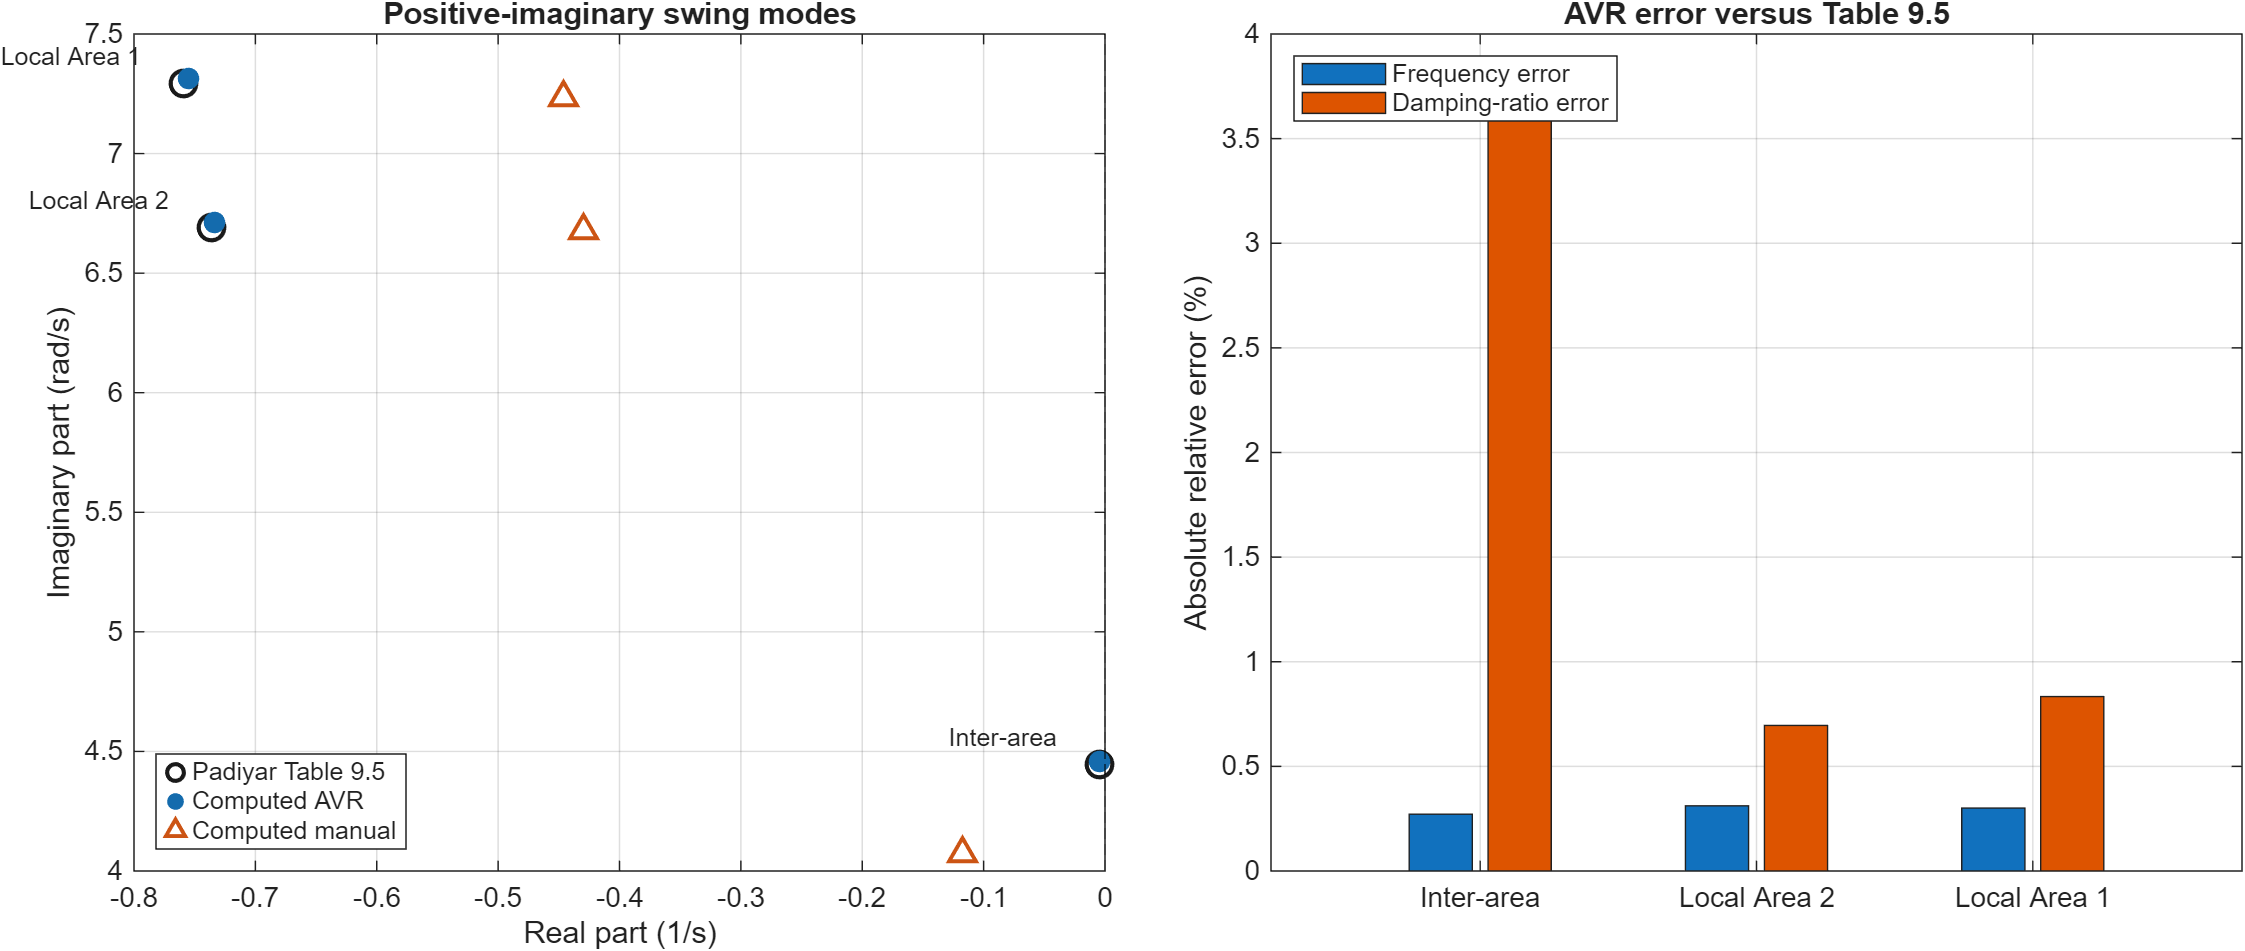
\includegraphics[width=\textwidth]{figures/padiyar_two_area/swing_mode_comparison.png}
\caption{Graphical counterpart of Table~10. Left: positive-imaginary
swing-mode eigenvalues. Right: AVR frequency and damping-ratio errors relative
to the published values. The manual case is plotted only in the complex plane
because no published manual-excitation target exists.}
\end{figure}


The AVR case reproduces the published mode groups without copying the table.
Differences are reported as model/numerical discrepancies rather than removed
by calibration. Manual excitation is a separate 16-state study and is not
expected to reproduce the 20-state AVR table.

\section{Time-Domain Simulation}

The source pages specify no time-domain fault scenario. For a controlled comparison,
this report defines a project scenario: a temporary balanced fault at bus~101,
$Z_f=j(10\times10^{-5})=j10^{-4}$ pu, applied at 1.0~s and cleared at 1.1~s,
simulated from 0 to 20.0~s with $\Delta t=0.005$~s.
The same network, operating point and disturbance are used for manual and AVR
configurations. The method uses a fixed nominal time step, exact event samples,
and an iterative implicit-trapezoidal corrector.

\subsection{Implicit trapezoidal integration}

\subsubsection{Why the implicit trapezoidal method is used}

This choice is numerical, not a post-result fit to a desired trajectory.  The
implemented Padiyar model is a semi-explicit differential--algebraic system
\begin{equation}
 \dot{x}=f(x,y,u),\qquad 0=g(x,y,Y),
 \label{eq:ts-dae-interface}
\end{equation}
in which the machine states $x$ evolve together with the algebraic network
voltages $y$.  Applying trapezoidal quadrature to the differential equation
over one interval of length $h$ gives
\begin{equation}
 x_{n+1}=x_n+\frac{h}{2}\left[f(x_n,y_n,u_n)
                  +f(x_{n+1},y_{n+1},u_{n+1})\right],
 \qquad g(x_{n+1},y_{n+1},Y_{n+1})=0.
 \label{eq:ts-trapezoidal-update}
\end{equation}
Equation~\eqref{eq:ts-trapezoidal-update} is the equation actually solved by
\path{stability.ts_step_kernel}; the algebraic endpoint condition is solved by
\path{stability.ts_algebraic_solve}.  The following rationale is a project
derivation from that implemented equation, rather than a claim that a reference
prints the project code verbatim.

First, for a smooth exact solution, Taylor expansion about $t_n$ gives the
one-step defect
\begin{equation}
x(t_n+h)-x(t_n)-\frac{h}{2}\left[\dot{x}(t_n)+\dot{x}(t_n+h)\right]
=-\frac{h^3}{12}x^{(3)}(t_n)+\mathcal{O}(h^4).
\label{eq:ts-trapezoidal-order}
\end{equation}
Thus trapezoidal quadrature has one-step truncation error
$\mathcal{O}(h^3)$ and global order two.  It therefore
improves the time-discretisation accuracy over first-order backward Euler at
the same nominal step while retaining an implicit endpoint solve.  Second,
its linear stability can be seen without relying on a plot.  For the test
equation $\dot{x}=\lambda x$, with $z=h\lambda$, the update becomes
\begin{equation}
 x_{n+1}=R(z)x_n,\qquad
 R(z)=\frac{1+z/2}{1-z/2}.
 \label{eq:ts-trapezoidal-stability}
\end{equation}
If $\operatorname{Re}(z)\le0$, then
$|1-z/2|^2-|1+z/2|^2=-2\operatorname{Re}(z)\ge0$, so
$|R(z)|\le1$.  The method is therefore A-stable: stable continuous modes are
not made unstable merely because an explicit method's stability region is too
small.  This is useful for the coupled machine--network DAE, whose electrical
and electromechanical modes can have substantially different time scales.
The step size is nevertheless selected for accuracy and event resolution, not
made arbitrarily large merely because the method is A-stable.

Third, the implicit endpoint formulation permits the network constraint
$g=0$ to be re-solved at each accepted endpoint.  When a fault is applied or
cleared, the integration grid lands exactly on the declared event time, the
network topology is switched, and the algebraic voltage is re-solved under the
new topology.  Thus the stored event sample is consistent with the DAE rather
than being obtained by interpolating across a discontinuous network change.

The method also has limitations.  It is not L-stable because
$R(z)\rightarrow-1$ as $z\rightarrow-\infty$; very fast decaying components
are not annihilated in one large step and can appear as numerical ringing if
$h$ is chosen too large.  Every step also requires nonlinear corrector and
algebraic Newton iterations.  The implementation therefore checks both the
trapezoidal residual and the algebraic residual and fails closed when those
iterations do not converge.  These accuracy and convergence checks, rather
than A-stability alone, justify an accepted TDS result.

The topology input is piecewise constant:
\begin{equation}
Y(t)=
\begin{cases}
Y_{pre},&t<t_f,\\
Y_{fault},&t_f\le t<t_c,\\
Y_{post},&t\ge t_c,
\end{cases}
\qquad
Y_{fault}=Y_{pre}+\frac{1}{Z_f}e_fe_f^T.
\label{eq:ts-topology}
\end{equation}
Here $e_f$ selects the faulted bus. Times $t_f$ and $t_c$ are inserted exactly
into the nominal $\Delta t$ grid, so no step hides a topology transition.

At each accepted state $x$, the network voltage is obtained from
\begin{equation}
g(x,y,Y)=0.
\label{eq:ts-algebraic}
\end{equation}
For algebraic Newton iteration $k$, set
$r_g^{(k)}=g(x,y^{(k)},Y)$ and $G_y^{(k)}=\partial g/\partial y$. Then
\begin{equation}
G_y^{(k)}\Delta y^{(k)}=-r_g^{(k)},\qquad
y^{(k+1)}=y^{(k)}+\alpha_k\Delta y^{(k)}.
\label{eq:ts-network-newton}
\end{equation}
The line search tries $\alpha_k=1,1/2,1/4,\ldots,2^{-16}$ and accepts the
first value that decreases $\|r_g\|_\infty$. The algebraic solve requires
$\|r_g\|_\infty\le10^{-11}$ and refreshes $G_y$ by central differences if
a step is rejected.

For $h=t_{n+1}-t_n$ and $f_n=f(x_n,y_n,u_n)$, the predictor is
\begin{equation}
\hat x^{(0)}_{n+1}=x_n+h f_n,\qquad
\hat y^{(0)}_{n+1}=y_n.
\label{eq:ts-predictor}
\end{equation}
Corrector iteration $c$ performs the following sequence:
\begin{align}
g(\hat x^{(c)}_{n+1},\hat y^{(c)}_{n+1},Y_n)&=0,\\
x^{(c+1)}_{n+1}
 &=x_n+\frac{h}{2}\left[f_n+
 f(\hat x^{(c)}_{n+1},\hat y^{(c)}_{n+1},u_n)\right],\\
g(x^{(c+1)}_{n+1},y^{(c+1)}_{n+1},Y_n)&=0,\\
R^{(c+1)}_{trap}
 &=x^{(c+1)}_{n+1}-x_n-\frac{h}{2}\left[f_n+
 f(x^{(c+1)}_{n+1},y^{(c+1)}_{n+1},u_n)\right].
\label{eq:ts-corrector}
\end{align}
The next iterate uses
$\hat x^{(c+1)}_{n+1}=x^{(c+1)}_{n+1}$. Acceptance requires both
\begin{equation}
\|x^{(c+1)}_{n+1}-\hat x^{(c)}_{n+1}\|_\infty\le\tau_n,
\qquad
\|R^{(c+1)}_{trap}\|_\infty\le\tau_n,
\end{equation}
where the implemented mixed tolerance is
\begin{equation}
\tau_n=10^{-10}+10^{-8}\max\left(1,\|x^{(c+1)}_{n+1}\|_\infty\right).
\end{equation}
At most 12 corrector iterations are allowed. A failed corrector raises an error
instead of accepting the step. After acceptance, $Y(t_{n+1})$ is selected
again and \eqref{eq:ts-algebraic} is solved, ensuring that a stored event
sample is consistent with the new topology.

\subsection{Fixed corrector iteration versus adaptive time stepping}

The corrector iteration and the time-step controller solve different problems.
For fixed $h$, repeated correction drives the nonlinear equation residual
\begin{equation}
F_h(x_{n+1})=
x_{n+1}-x_n-\frac{h}{2}\left(f_n+f_{n+1}\right)
\end{equation}
toward zero. Thus $\|F_h\|_\infty\ll1$ proves that the trapezoidal equation
for the chosen $h$ was solved accurately. It does not estimate the discretization
error $\|x(t_{n+1})-x_{n+1}\|$.

An adaptive second-order trapezoidal method additionally needs an independent
local-error estimate. Step doubling would compute one full step $x_h$ and two
half steps $x_{h/2,h/2}$, then form
\begin{equation}
e_n=\frac{x_{h/2,h/2}-x_h}{2^2-1},\qquad
E_n=\left\|
\frac{e_n}{a_{tol}+r_{tol}\max(|x_n|,|x_{h/2,h/2}|)}
\right\|_\infty.
\label{eq:adaptive-estimator}
\end{equation}
The step is accepted only when $E_n\le1$; otherwise it is rejected and
recomputed. A typical controller is
\begin{equation}
h_{new}=h\,
\operatorname{clip}\left(f_{min},f_{max},
safety\,E_n^{-1/3}\right),
\label{eq:adaptive-controller}
\end{equation}
with event times imposing an upper bound on $h_{new}$ so the solver still lands
exactly on $t_f$ and $t_c$.

The present validation solver intentionally remains fixed-step because the
published comparison protocol requires a deterministic common output grid and
the implementation currently has neither the independent estimator
\eqref{eq:adaptive-estimator} nor step rejection. Calling corrector iteration
adaptive would therefore be false. Fixed $h=0.005$~s is accepted here only
after equilibrium, residual, convergence, and finite-trajectory checks; it is
not presented as a general proof of time-discretization accuracy. Adaptive
stepping is a valid future production improvement, but it must add the
estimator, accept/reject controller, exact event landing, resampling for
cross-tool comparison, and convergence tests under successively tighter
tolerances before replacing this reproducible validation path.

The recorded outputs are reconstructed from the accepted $(x_n,y_n)$:
\begin{equation}
|V_b|=\sqrt{y_{2b-1}^2+y_{2b}^2},\qquad
P_{ei}=V_{di}I_{di}+V_{qi}I_{qi}+R_a(I_{di}^2+I_{qi}^2),
\end{equation}
with $P_{ei}[\mathrm{MW}]=S_{base}[\mathrm{MVA}]P_{ei}[\mathrm{pu}]$.
The saved diagnostics include the initial DAE residual, corrector update norm,
trapezoidal residual, iteration count, convergence flag, and non-converged-step
count; consequently, a plausible plot cannot conceal a failed numerical step.

\begin{table}[H]\centering
\caption{Time-domain-simulation input contract, numerical status, and response
extrema for the 0--20~s bus-101 fault scenario with
$Z_f=j10^{-4}$~pu, $t_f=1.0$~s, $t_c=1.1$~s, and
$\Delta t=0.005$~s.}
\label{tab:ts-summary}
\begin{tabular}{llrr}\toprule {Metric} & {Unit} & {AVR} & {Manual excitation}\\ \midrule
Initial DAE residual & pu & 9.215e-13 & 5.684e-14\\
Non-converged steps & steps & 0 & 0\\
Maximum corrector residual & pu & 7.676e-09 & 5.107e-10\\
Minimum bus voltage & pu & 0.9244 & 0.9184\\
Maximum speed deviation & pu & 4.397e-04 & 8.002e-04\\
\bottomrule\end{tabular}

\end{table}

\begin{figure}[H]\centering
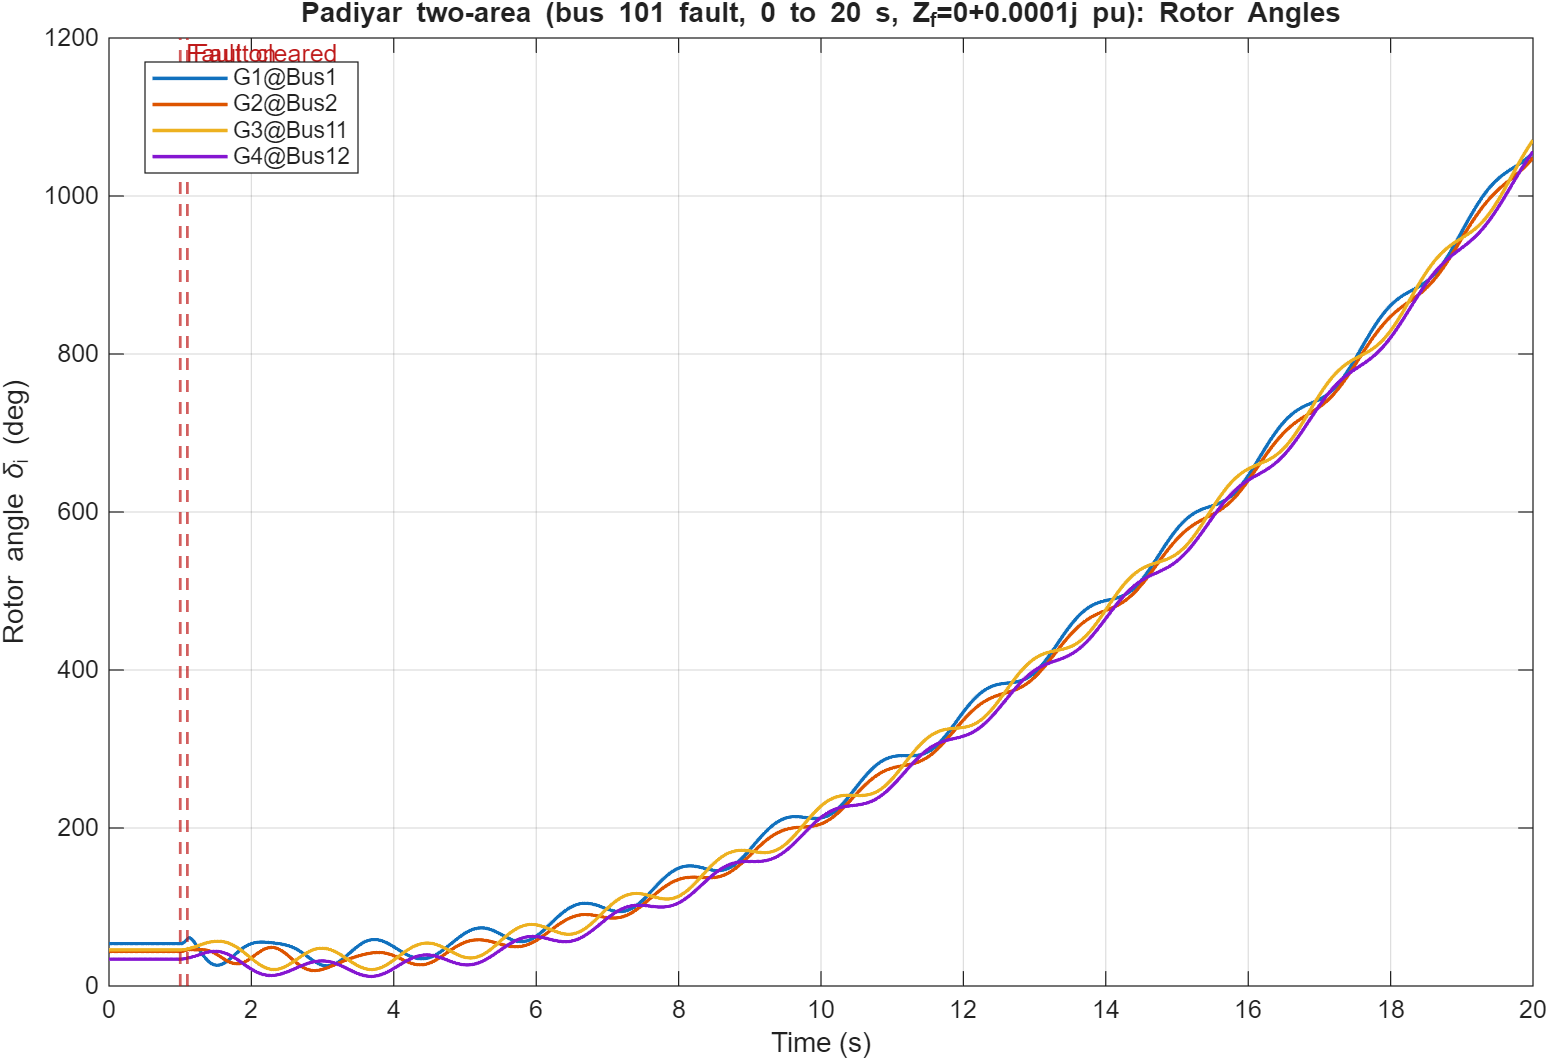
\includegraphics[width=.90\textwidth]{figures/padiyar_two_area/fault_comparison.png}
\caption{Bus-101 project fault response using the AVR configuration (the
book's 20-state model): stored absolute generator rotor angles
$\delta_i(t)$ in degrees. No initial-angle subtraction is applied. Red
markers identify fault application and clearance. The simulated interval is
0--20~s and $Z_f=j10^{-4}$~pu.}
\label{fig:ts-avr-angle}
\end{figure}

\begin{figure}[H]\centering
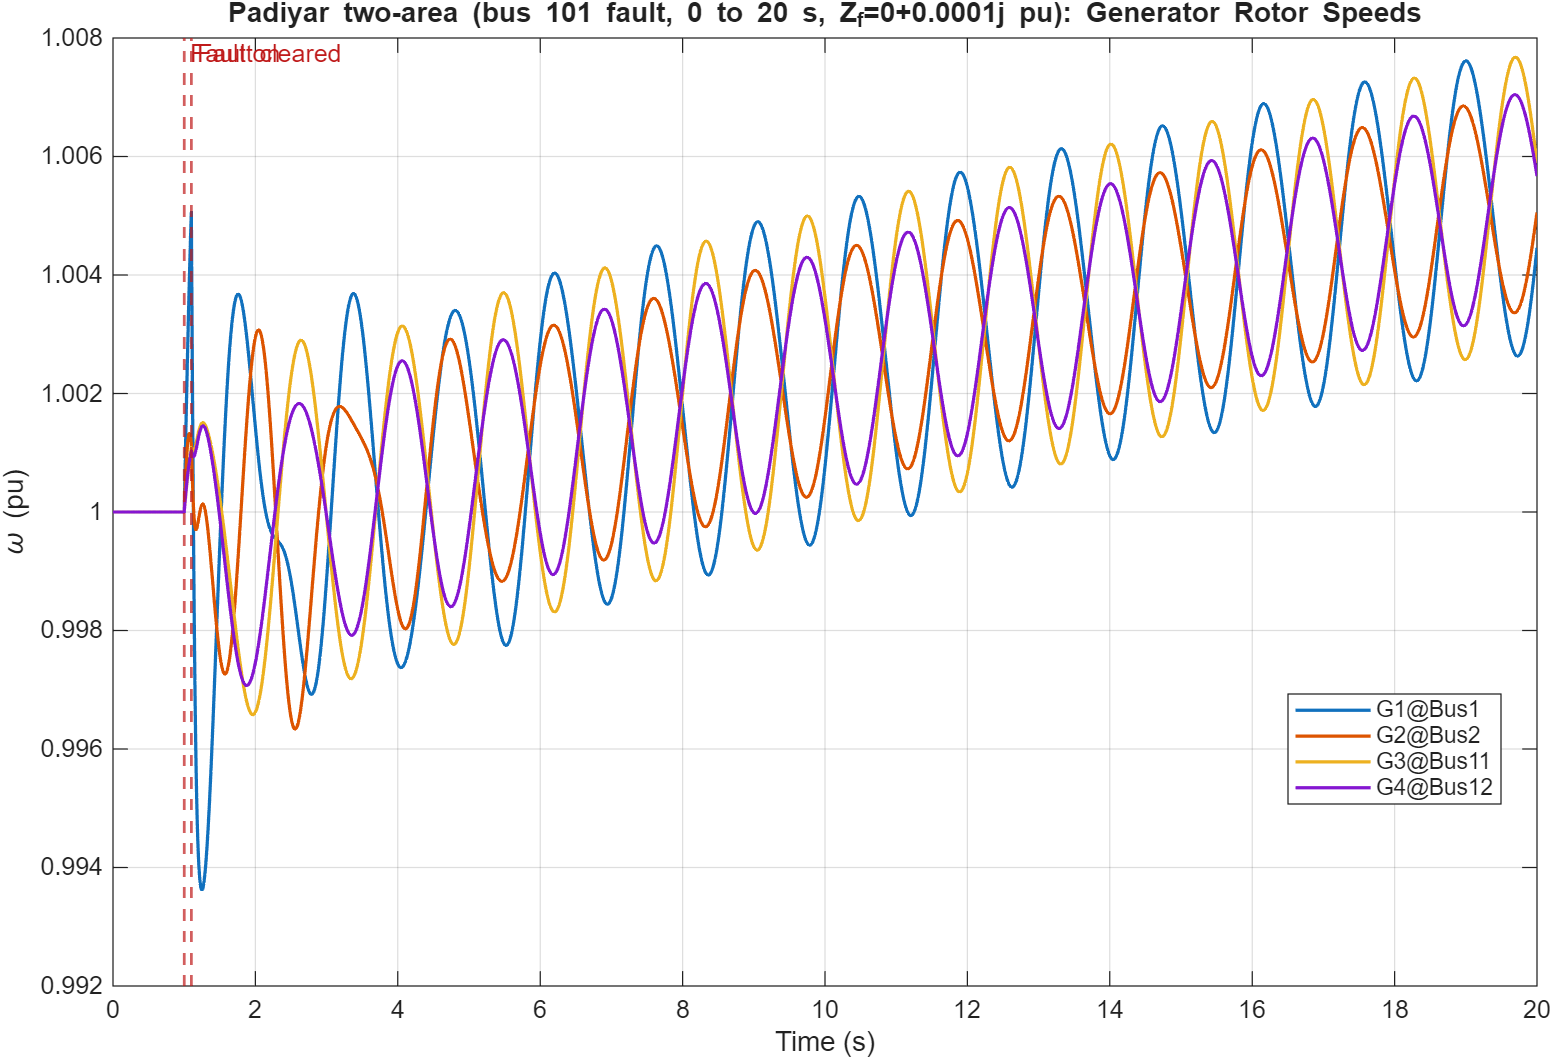
\includegraphics[width=.90\textwidth]{figures/padiyar_two_area/fault_comparison_omega.png}
\caption{Bus-101 project fault response using the AVR configuration:
stored absolute rotor speeds $\omega_i(t)$ in per unit. The plotted values
are the TS result values themselves; the graph does not plot $\omega_i-1$.
The simulated interval is 0--20~s and $Z_f=j10^{-4}$~pu.}
\label{fig:ts-avr-omega}
\end{figure}

\begin{figure}[H]\centering
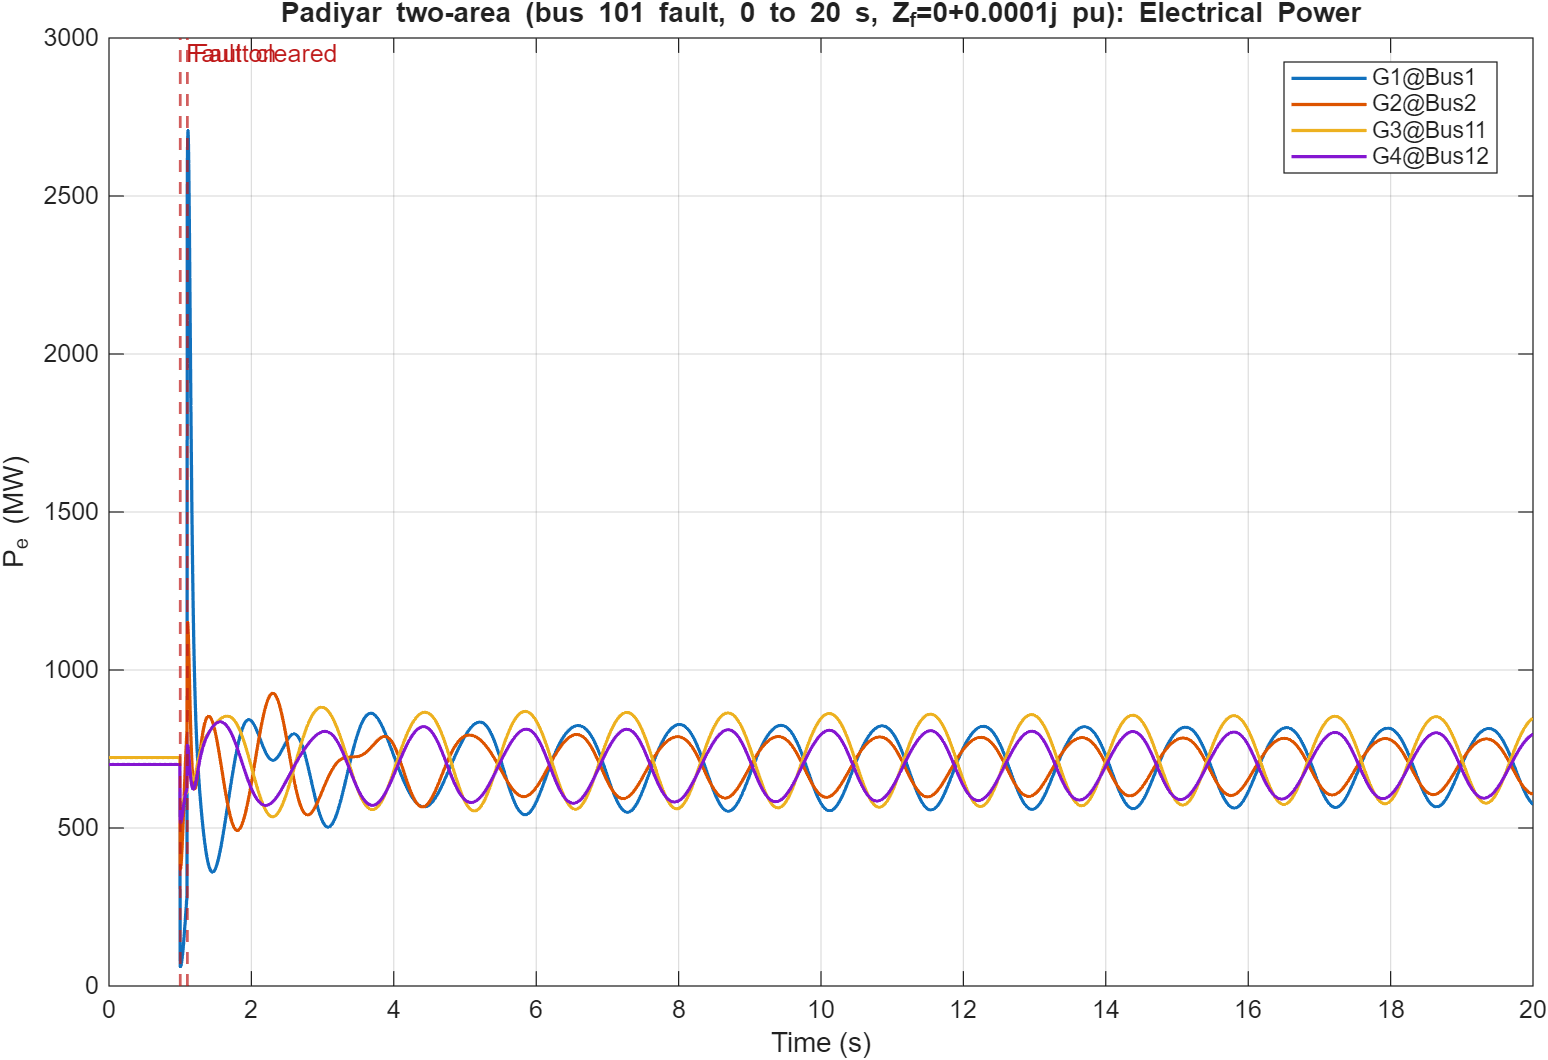
\includegraphics[width=.90\textwidth]{figures/padiyar_two_area/fault_comparison_pe.png}
\caption{Bus-101 project fault response using the AVR configuration:
generator air-gap electrical powers $P_{ei}(t)$ reconstructed from the
accepted TS states and algebraic bus voltages. The simulated interval is
0--20~s and $Z_f=j10^{-4}$~pu.}
\label{fig:ts-avr-pe}
\end{figure}

\begin{figure}[H]\centering
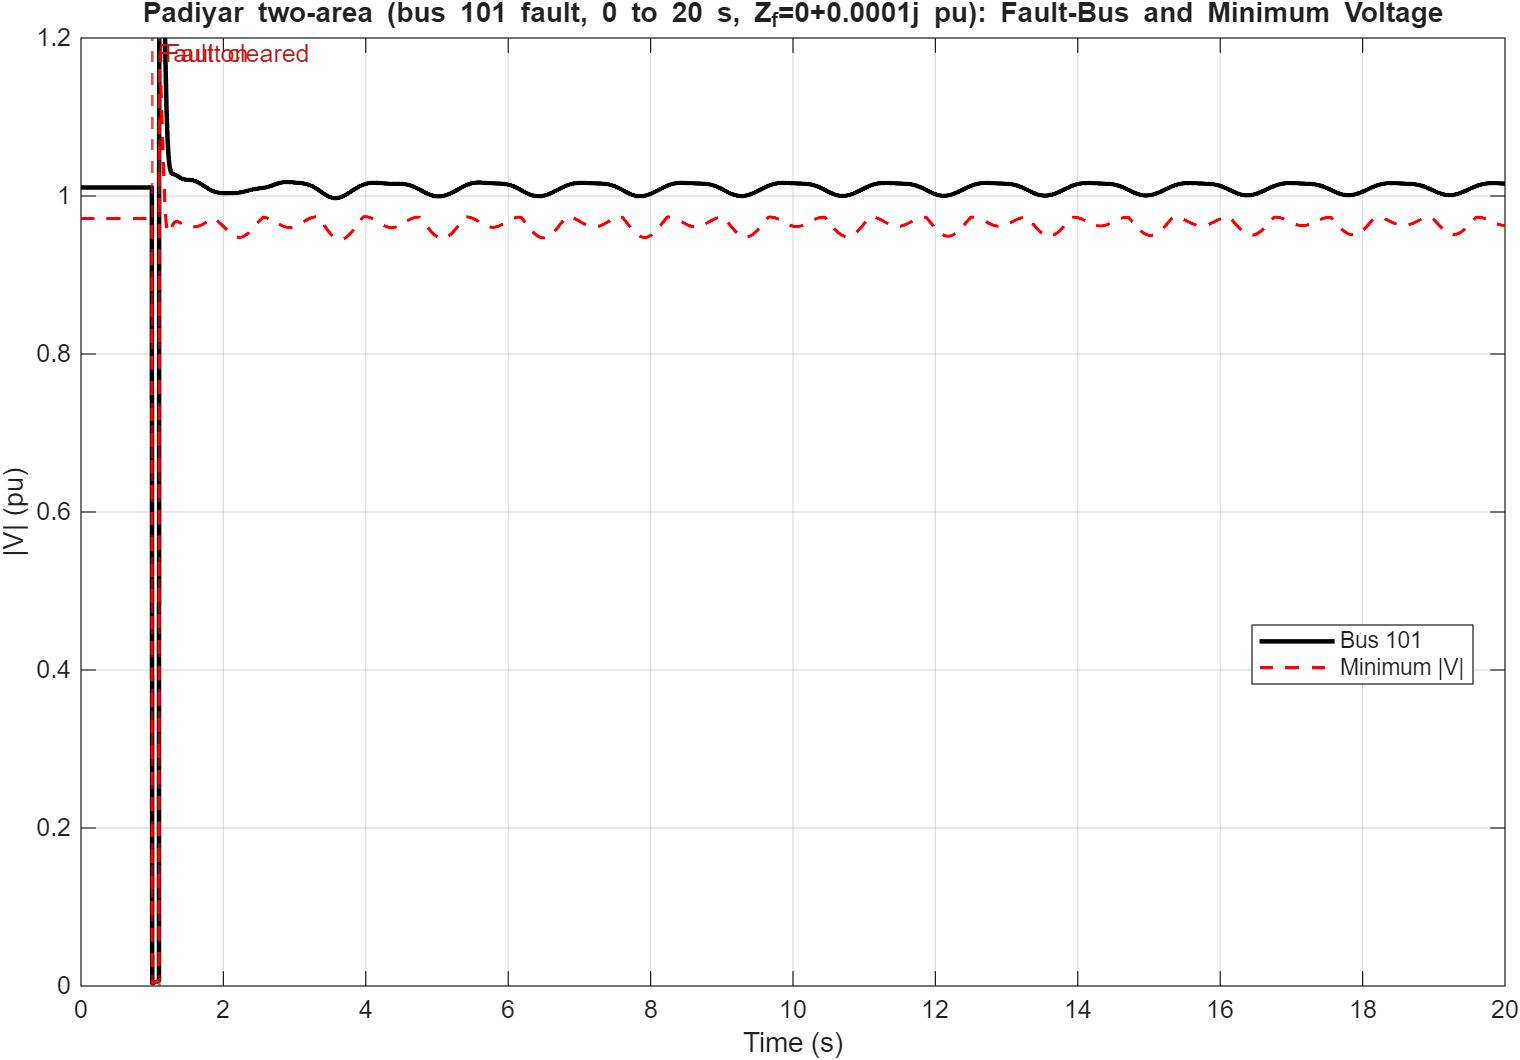
\includegraphics[width=.90\textwidth]{figures/padiyar_two_area/fault_comparison_voltage.png}
\caption{Bus-101 project fault response using the AVR configuration:
fault-bus voltage magnitude and the minimum voltage magnitude across the
network. The simulated interval is 0--20~s and $Z_f=j10^{-4}$~pu.}
\label{fig:ts-avr-voltage}
\end{figure}

\begin{figure}[H]\centering
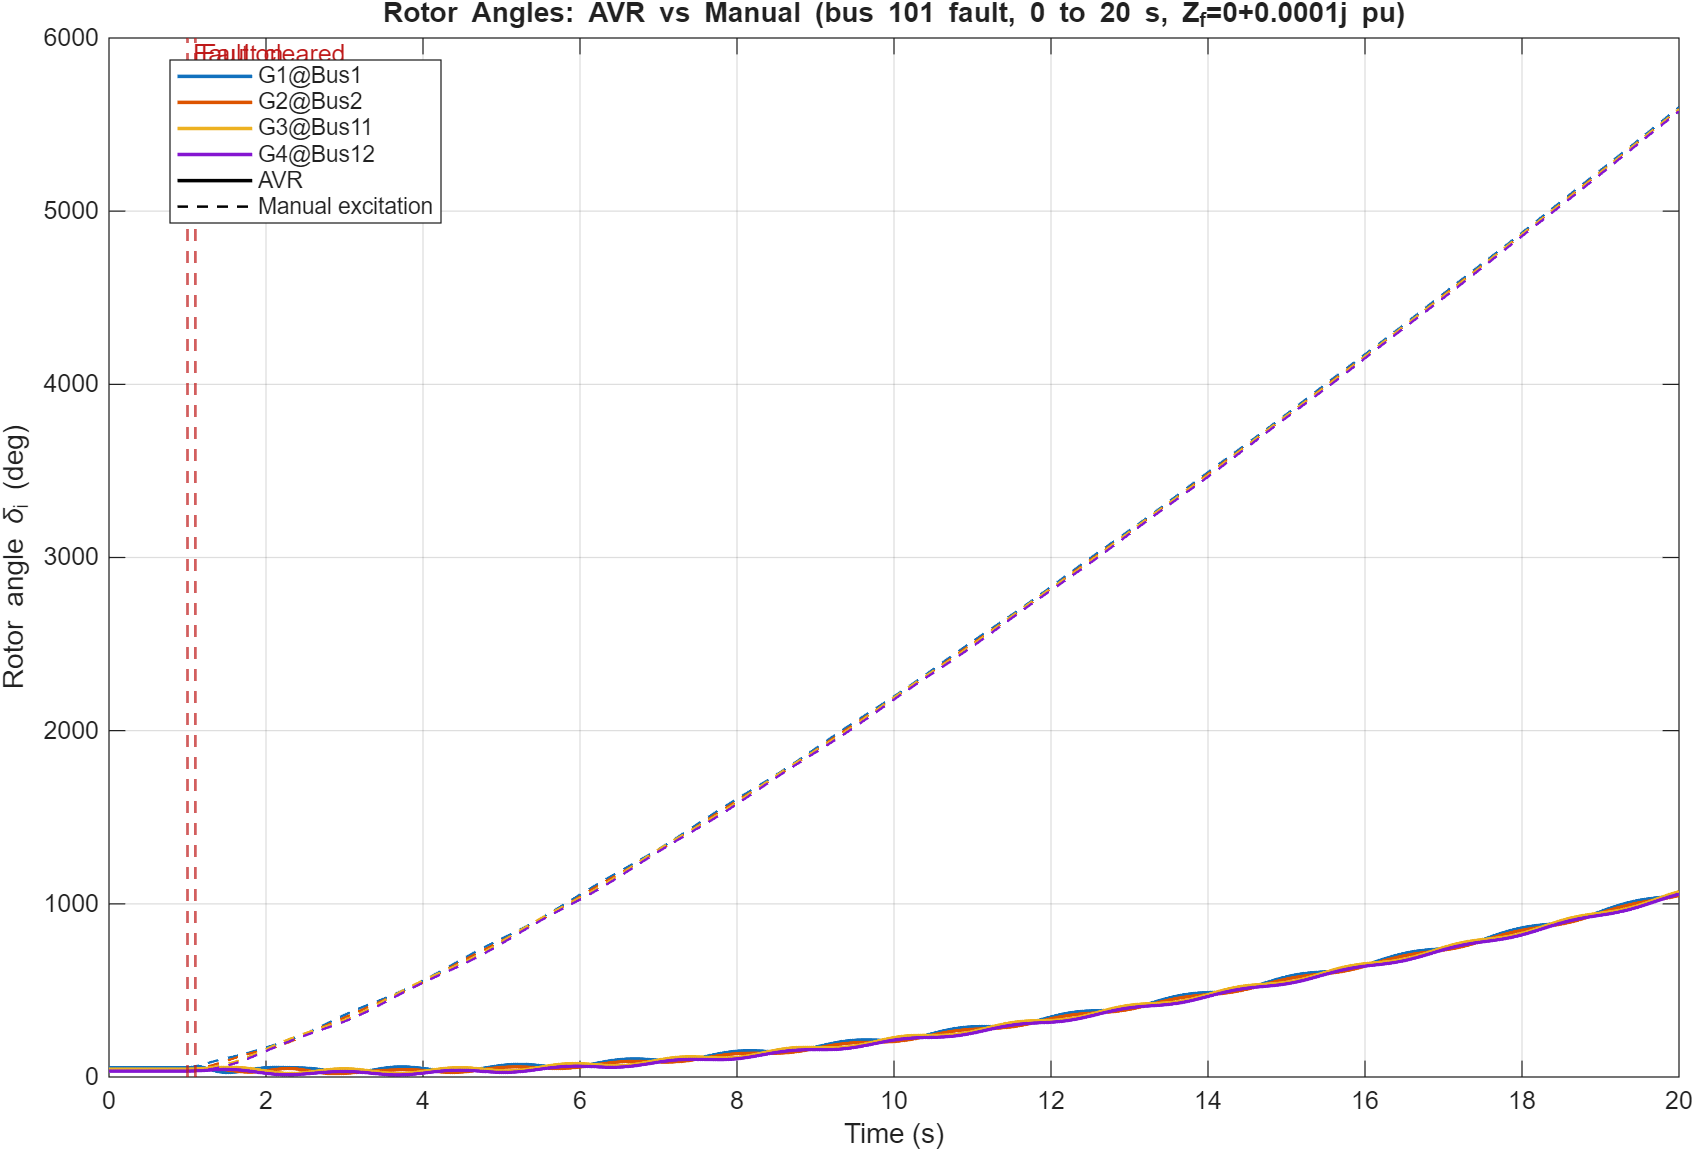
\includegraphics[width=.90\textwidth]{figures/padiyar_two_area/ts_avr_vs_manual.png}
\caption{Stored absolute rotor angles for the bus-101 fault: AVR (solid)
versus manual excitation (dashed). Each colour identifies one generator.
No initial-angle subtraction is applied. The simulated interval is 0--20~s
and $Z_f=j10^{-4}$~pu.}
\label{fig:ts-comparison-angle}
\end{figure}

\begin{figure}[H]\centering
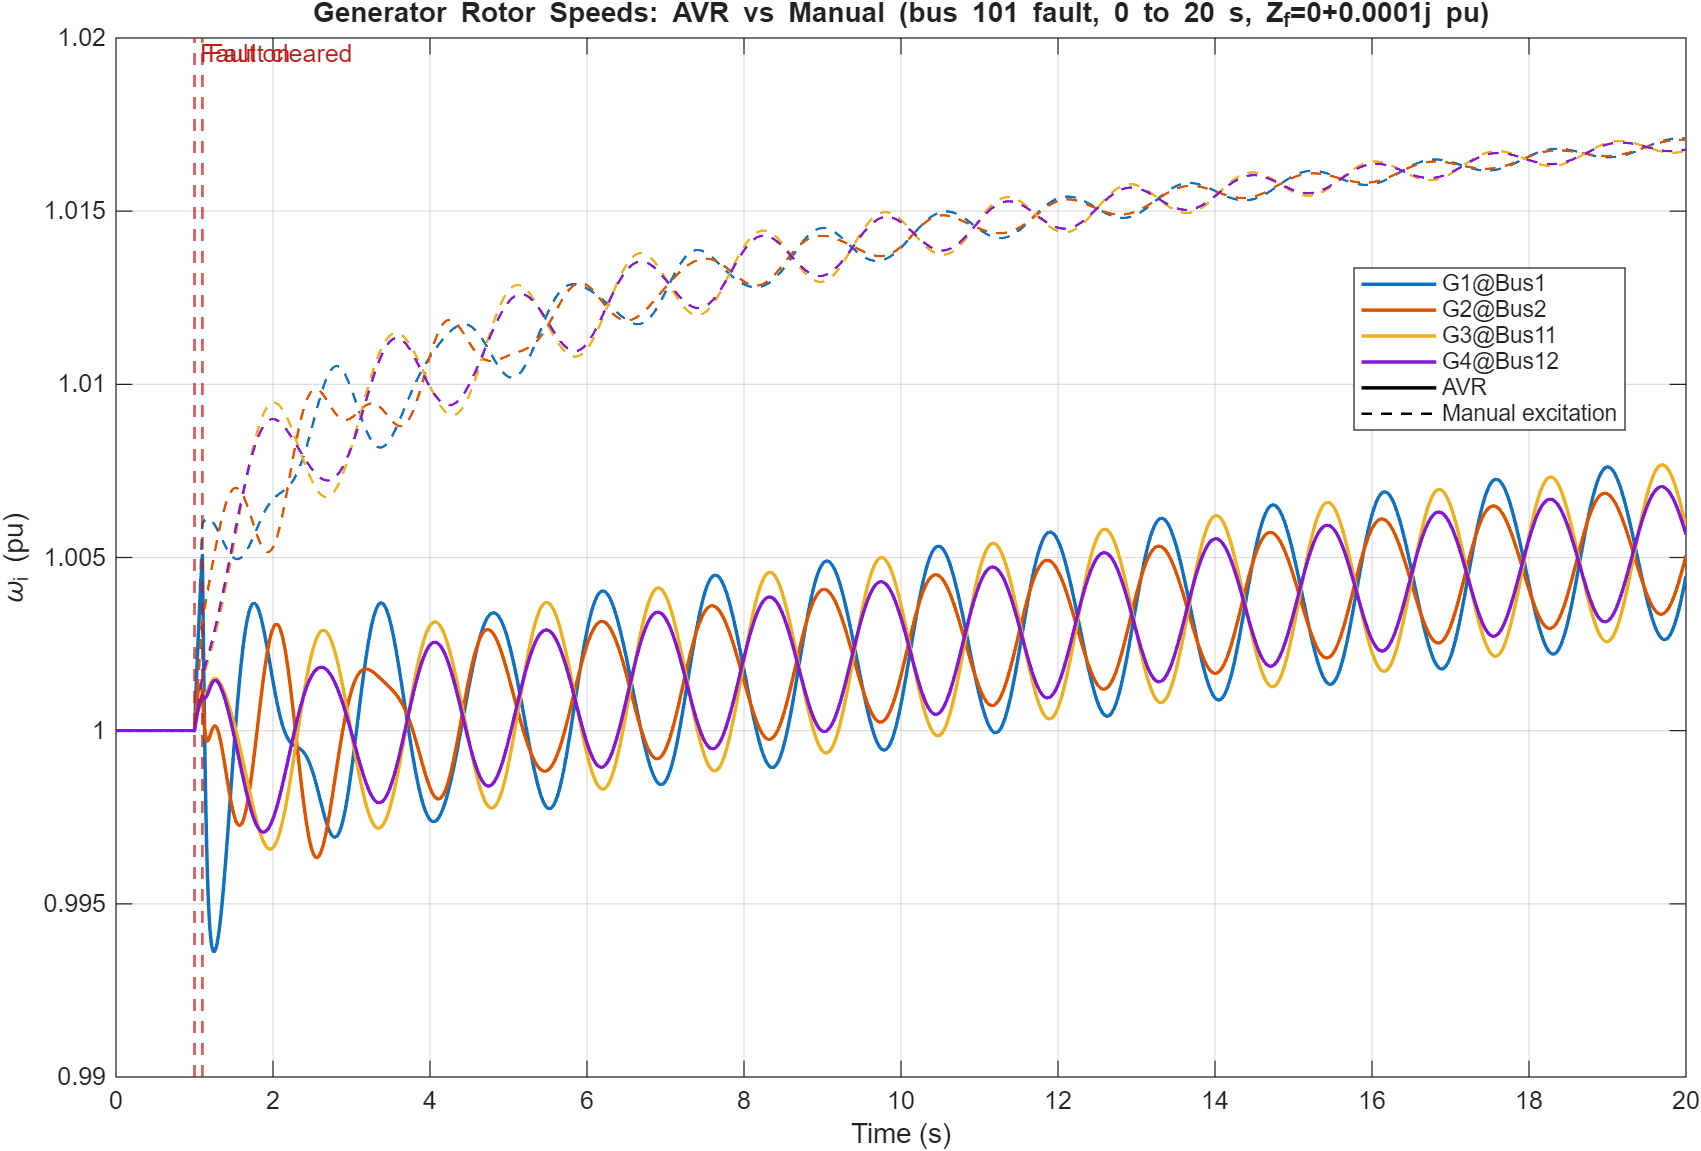
\includegraphics[width=.90\textwidth]{figures/padiyar_two_area/ts_avr_vs_manual_omega.png}
\caption{Stored absolute rotor speeds $\omega_i(t)$ for the bus-101 fault:
AVR (solid) versus manual excitation (dashed). No $\omega_i-1$ plotting
transform is applied. The simulated interval is 0--20~s and
$Z_f=j10^{-4}$~pu.}
\label{fig:ts-comparison-omega}
\end{figure}

\begin{figure}[H]\centering
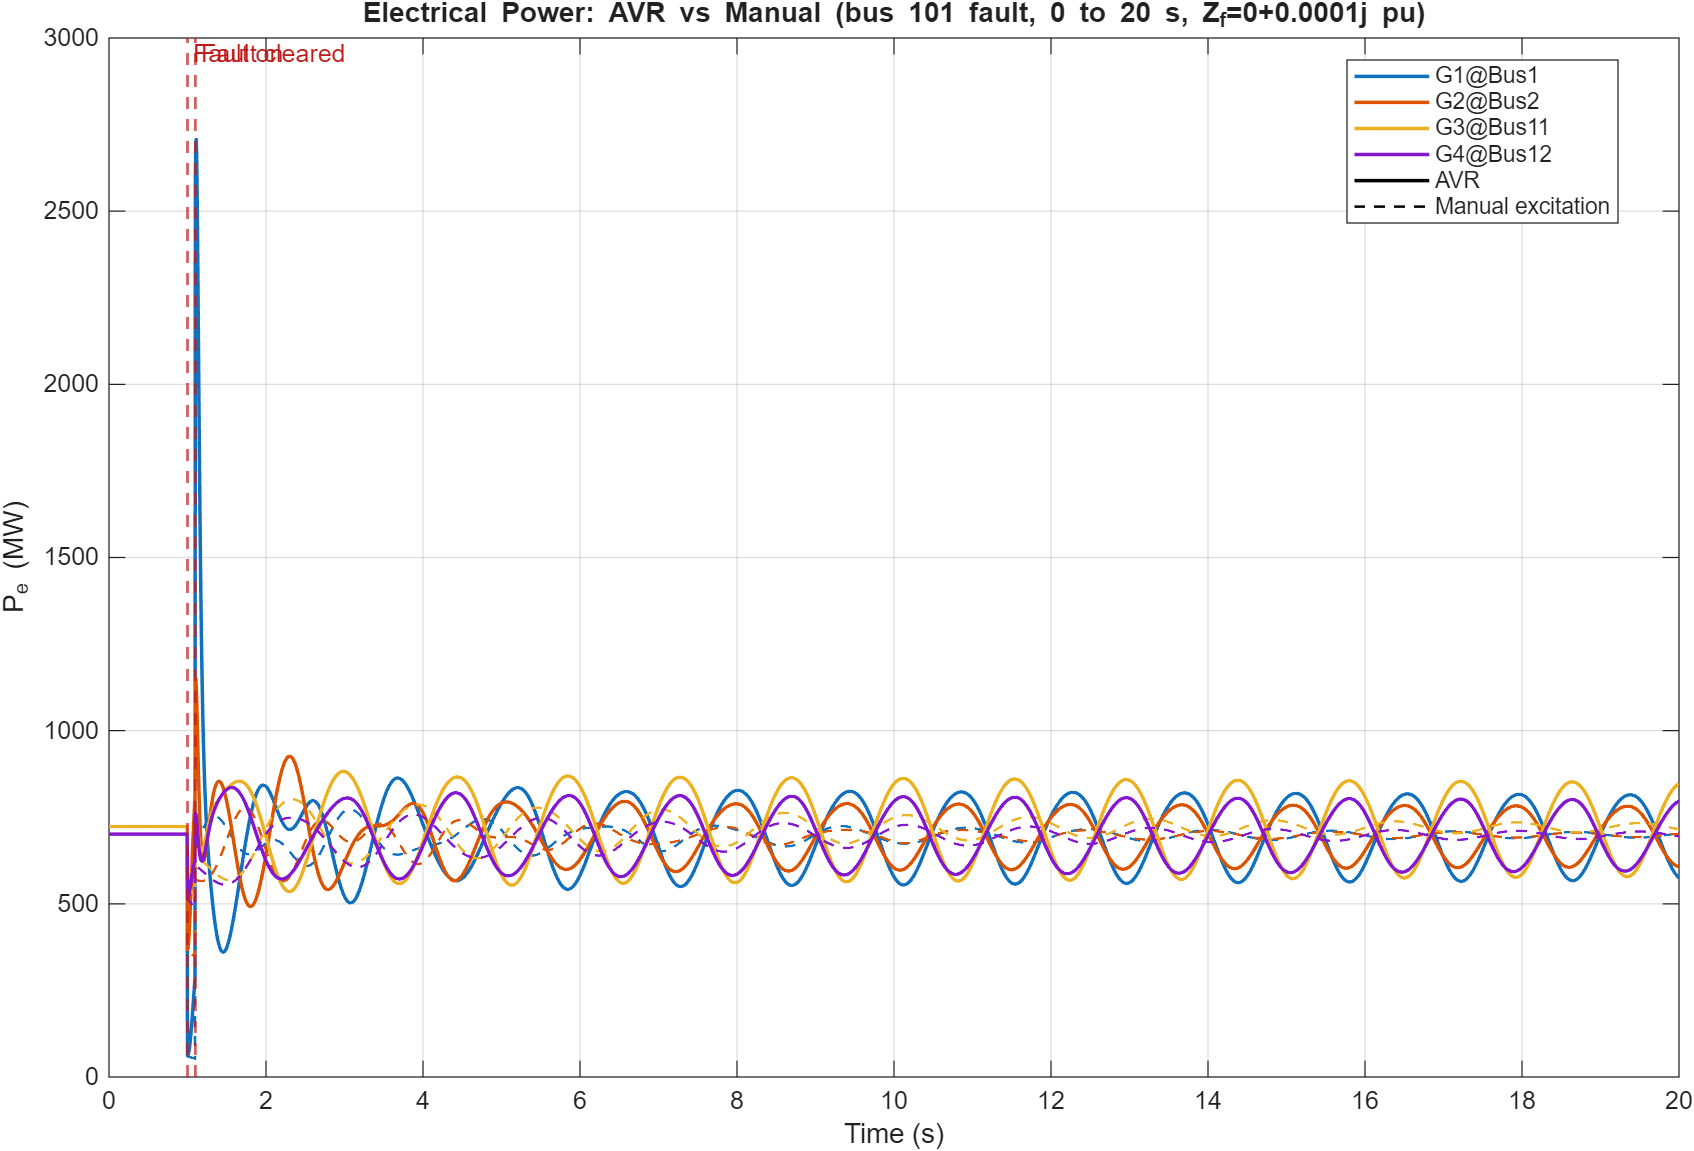
\includegraphics[width=.90\textwidth]{figures/padiyar_two_area/ts_avr_vs_manual_pe.png}
\caption{Generator electrical powers for the bus-101 fault: AVR (solid)
versus manual excitation (dashed). The simulated interval is 0--20~s and
$Z_f=j10^{-4}$~pu.}
\label{fig:ts-comparison-pe}
\end{figure}

\begin{figure}[H]\centering
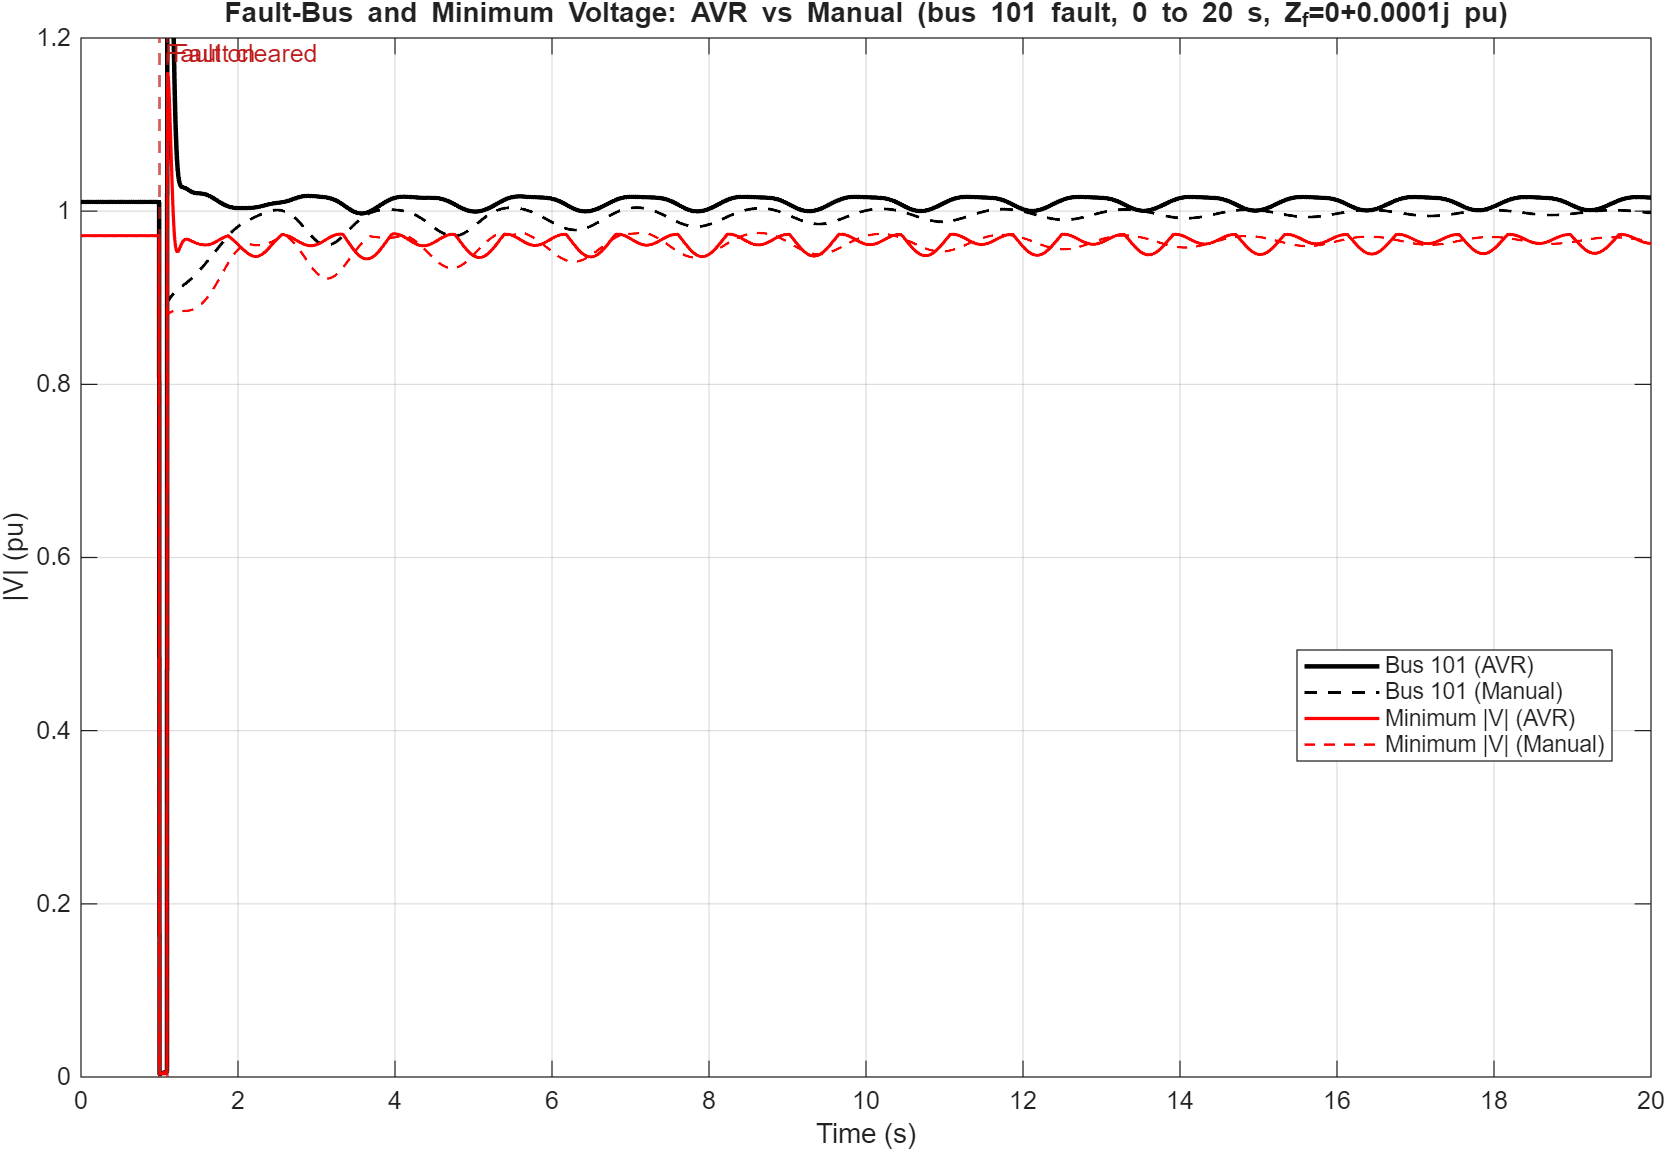
\includegraphics[width=.90\textwidth]{figures/padiyar_two_area/ts_avr_vs_manual_voltage.png}
\caption{Fault-bus and minimum network voltage magnitudes for the bus-101
fault: AVR (solid) versus manual excitation (dashed). Quantitative modal
damping is determined from \eqref{eq:sssa-modal-metrics} and Table~10, not
inferred from visual appearance. The simulated interval is 0--20~s and
$Z_f=j10^{-4}$~pu.}
\label{fig:ts-comparison-voltage}
\end{figure}

\section{IEEE 14-bus cross-validation against PSAT}

This section cross-validates the common classical PF, SSSA and TDS substrate
against PSAT~2.1.11. It is an independent infrastructure check and is not a
claim that PSAT implements the five-state Padiyar model used in the preceding
sections. Every IEEE14 table and figure below is generated in the same
invocation as a fresh in-house run and a fresh PSAT run; no saved trajectory,
prior numeric table, or prior plot is read. The generating entry point is
\path{generate_padiyar_ieee14_psat_tables}.

\subsection{System description}

The network is the MATPOWER~6 IEEE 14-bus case converted into the project
schema. It has 14 bus rows, five in-service generator rows at buses
1, 2, 3, 6 and 8, and 20 in-service branch rows. The complete input inventory
used in this study is given before the computed PF, SSSA and TDS results.

\begin{figure}[H]
\centering
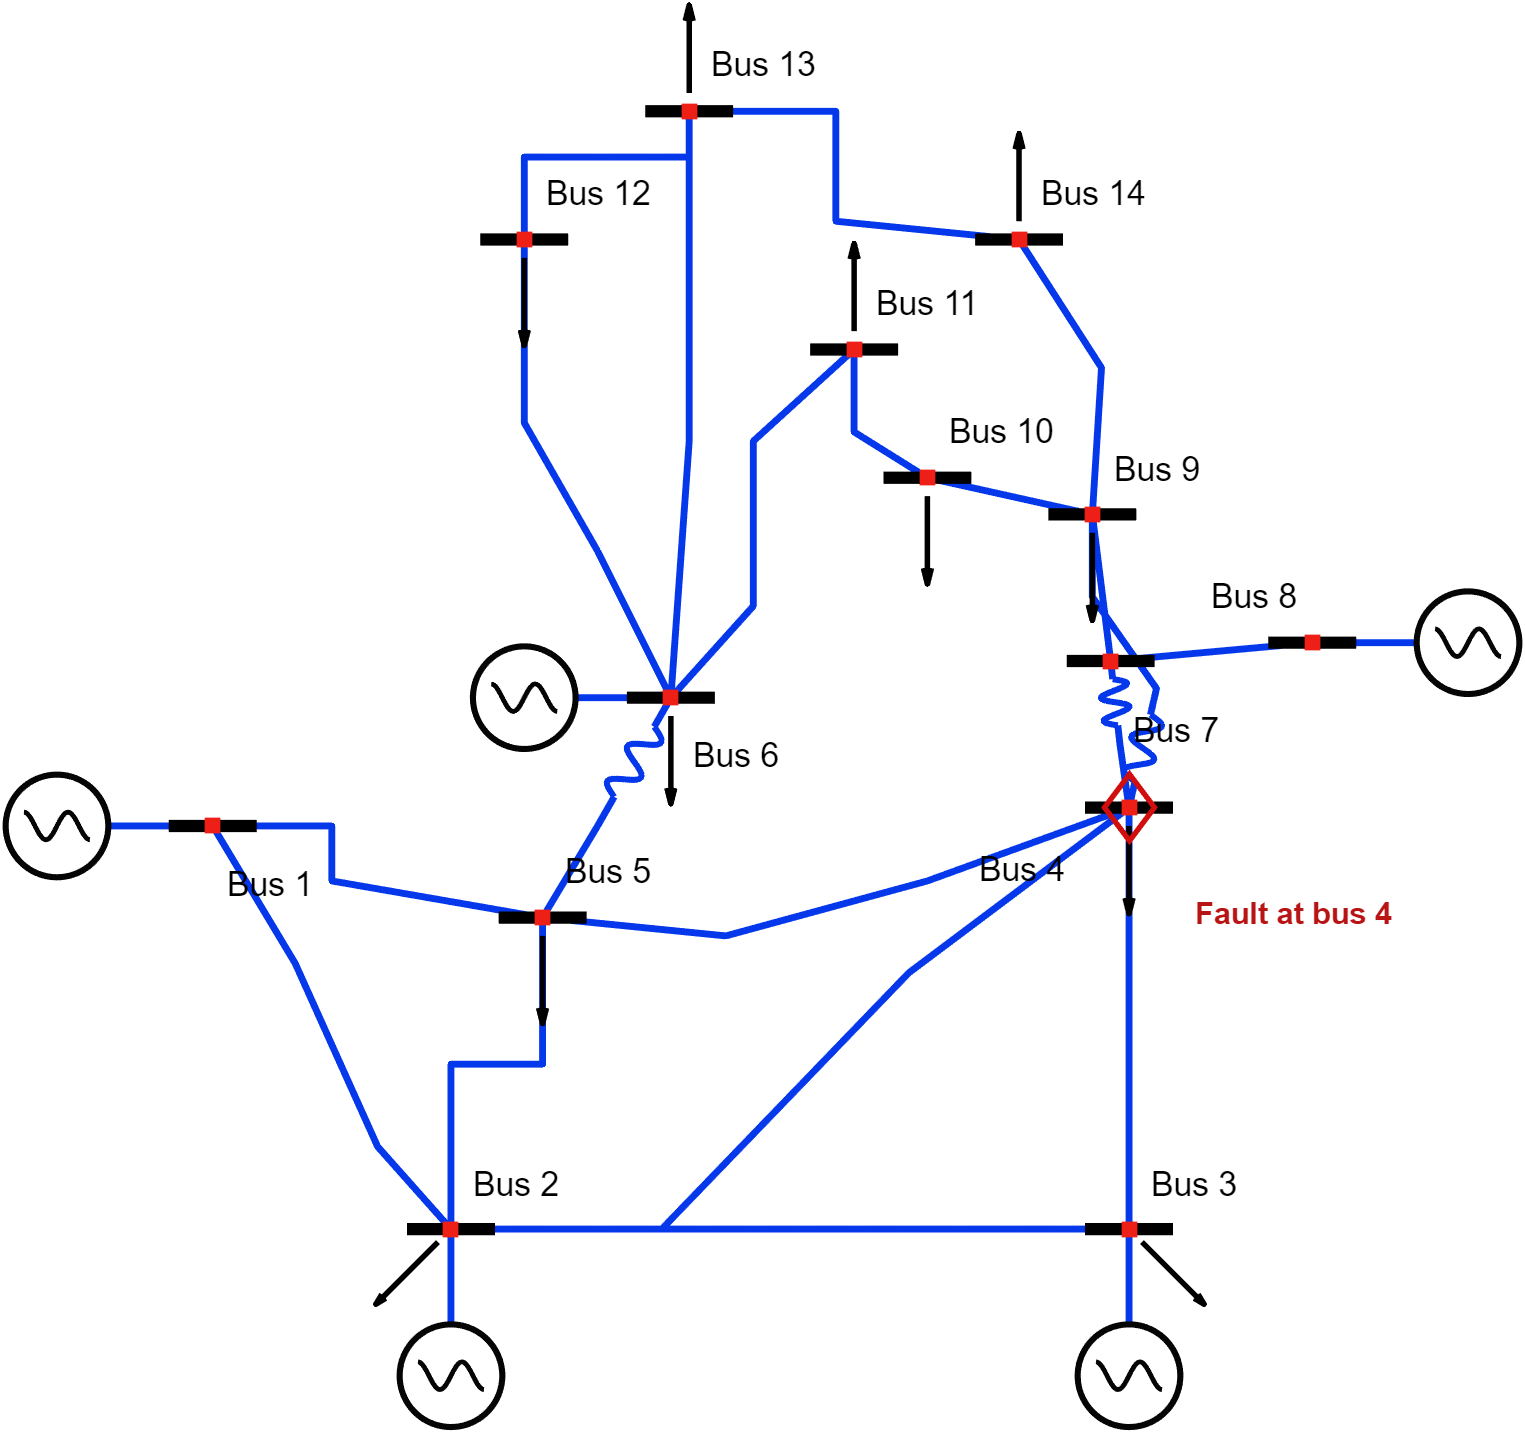
\includegraphics[width=.92\textwidth]{figures/padiyar_two_area/ieee14_network.png}
\caption{IEEE 14-bus network generated from the same MATPOWER branch, bus and
generator rows used by Our and PSAT. Generator buses, nonzero-load buses,
transformer branches and the bus-4 fault location are marked explicitly.}
\label{fig:ieee14-network}
\end{figure}

\subsection{Source data (MATPOWER IEEE 14-bus)}

\begin{table}[H]\centering\small
\caption{MATPOWER IEEE14 case summary: 14 buses, five online generators and
20 line/transformer rows, with the shared base quantities.}
\label{tab:ieee14-case-summary}
\resizebox{\textwidth}{!}{% Fresh case summary derived from the exact IEEE14 case used by both solvers.
\begin{tabular}{lll}\toprule
Item & Value & Contract note \\ \midrule
Case & {MATPOWER 6.0 IEEE 14-bus} & Converted from the supplied case14.m \\ 
Power base & 100 MVA & MATPOWER mpc.baseMVA \\ 
Nominal frequency & 60 Hz & Project dynamic base \\ 
Bus rows & 14 & 1 REF, 4 PV, 9 PQ \\ 
Online generators & 5 & Buses [1,2,3,6,8] \\ 
Online branches & 20 & 3 transformer-tap branches \\ 
Total specified demand & 259.0 MW, 73.5 MVAr & Sum of bus Pd and Qd \\ 
Nonzero shunt susceptance & 19.0 MVAr & Bus 9 source Bs entry \\ 
\bottomrule\end{tabular}
}
\end{table}

\subsubsection{Bus data and bus types}

Table~\ref{tab:ieee14-bus-data} records the source bus operating entries and
aggregated source generation. Table~\ref{tab:ieee14-bus-parameters} preserves
the remaining MATPOWER bus-matrix fields, including the bus type, shunt,
area, voltage limits and initial voltage. The source $P_G/Q_G$ entries are
case data; their input/output interpretation follows the effective REF, PV
and PQ bus types.

\begin{table}[H]\centering\small
\caption{IEEE14 bus-type assignment, including the MATPOWER type codes and
the buses in each REF, PV and PQ group.}
\label{tab:ieee14-bus-types}
\resizebox{.78\textwidth}{!}{% Fresh bus-type assignment from the exact IEEE14 bus matrix.
\begin{tabular}{l r l r}\toprule
Bus type & MATPOWER code & Bus IDs & Count \\ \midrule
REF & 3 & {[1]} & 1 \\ 
PV & 2 & {[2,3,6,8]} & 4 \\ 
PQ & 1 & {[4,5,7,9,10,11,12,13,14]} & 9 \\ 
\bottomrule\end{tabular}
}
\end{table}

\begin{table}[H]\centering\small
\caption{IEEE 14-bus data and bus types shared by the in-house and PSAT runs.}
\label{tab:ieee14-bus-data}
\resizebox{\textwidth}{!}{% Fresh source-data table generated in the same invocation as the IEEE14 simulations.
\begin{tabular}{r l r r r r r r}\toprule
Bus & Type & {$|V|_{src}$} & {$\theta_{src}$} & {$P_L$} & {$Q_L$} & {$P_G$} & {$Q_G$} \\
{} & {} & {(pu)} & {(deg)} & {(MW)} & {(MVAr)} & {(MW)} & {(MVAr)} \\ \midrule
1 & REF & 1.0600 & 0.0000 & 0.00 & 0.00 & 232.40 & -16.90 \\
2 & PV & 1.0450 & -4.9800 & 21.70 & 12.70 & 40.00 & 42.40 \\
3 & PV & 1.0100 & -12.7200 & 94.20 & 19.00 & 0.00 & 23.40 \\
4 & PQ & 1.0190 & -10.3300 & 47.80 & -3.90 & 0.00 & 0.00 \\
5 & PQ & 1.0200 & -8.7800 & 7.60 & 1.60 & 0.00 & 0.00 \\
6 & PV & 1.0700 & -14.2200 & 11.20 & 7.50 & 0.00 & 12.20 \\
7 & PQ & 1.0620 & -13.3700 & 0.00 & 0.00 & 0.00 & 0.00 \\
8 & PV & 1.0900 & -13.3600 & 0.00 & 0.00 & 0.00 & 17.40 \\
9 & PQ & 1.0560 & -14.9400 & 29.50 & 16.60 & 0.00 & 0.00 \\
10 & PQ & 1.0510 & -15.1000 & 9.00 & 5.80 & 0.00 & 0.00 \\
11 & PQ & 1.0570 & -14.7900 & 3.50 & 1.80 & 0.00 & 0.00 \\
12 & PQ & 1.0550 & -15.0700 & 6.10 & 1.60 & 0.00 & 0.00 \\
13 & PQ & 1.0500 & -15.1600 & 13.50 & 5.80 & 0.00 & 0.00 \\
14 & PQ & 1.0360 & -16.0400 & 14.90 & 5.00 & 0.00 & 0.00 \\
\bottomrule\end{tabular}
}
\end{table}

\begin{table}[H]\centering\scriptsize
\caption{MATPOWER IEEE14 bus data: complete bus-matrix parameters supplied to
the case converter.}
\label{tab:ieee14-bus-parameters}
\resizebox{\textwidth}{!}{% Fresh MATPOWER bus-matrix fields from the case used in this invocation.
\begin{tabular}{r l r r r r r r r r r r r}\toprule
Bus & Type & {$P_d$} & {$Q_d$} & {$G_s$} & {$B_s$} & Area & {$V_m$} & {$V_a$} & {baseKV} & Zone & {$V_{max}$} & {$V_{min}$} \\ 
{} & {} & {(MW)} & {(MVAr)} & {(MW)} & {(MVAr)} & {} & {(pu)} & {(deg)} & {(kV)} & {} & {(pu)} & {(pu)} \\ \midrule
1 & REF & 0.00 & 0.00 & 0.00 & 0.00 & 1 & 1.0600 & 0.0000 & 0.0 & 1 & 1.06 & 0.94 \\ 
2 & PV & 21.70 & 12.70 & 0.00 & 0.00 & 1 & 1.0450 & -4.9800 & 0.0 & 1 & 1.06 & 0.94 \\ 
3 & PV & 94.20 & 19.00 & 0.00 & 0.00 & 1 & 1.0100 & -12.7200 & 0.0 & 1 & 1.06 & 0.94 \\ 
4 & PQ & 47.80 & -3.90 & 0.00 & 0.00 & 1 & 1.0190 & -10.3300 & 0.0 & 1 & 1.06 & 0.94 \\ 
5 & PQ & 7.60 & 1.60 & 0.00 & 0.00 & 1 & 1.0200 & -8.7800 & 0.0 & 1 & 1.06 & 0.94 \\ 
6 & PV & 11.20 & 7.50 & 0.00 & 0.00 & 1 & 1.0700 & -14.2200 & 0.0 & 1 & 1.06 & 0.94 \\ 
7 & PQ & 0.00 & 0.00 & 0.00 & 0.00 & 1 & 1.0620 & -13.3700 & 0.0 & 1 & 1.06 & 0.94 \\ 
8 & PV & 0.00 & 0.00 & 0.00 & 0.00 & 1 & 1.0900 & -13.3600 & 0.0 & 1 & 1.06 & 0.94 \\ 
9 & PQ & 29.50 & 16.60 & 0.00 & 19.00 & 1 & 1.0560 & -14.9400 & 0.0 & 1 & 1.06 & 0.94 \\ 
10 & PQ & 9.00 & 5.80 & 0.00 & 0.00 & 1 & 1.0510 & -15.1000 & 0.0 & 1 & 1.06 & 0.94 \\ 
11 & PQ & 3.50 & 1.80 & 0.00 & 0.00 & 1 & 1.0570 & -14.7900 & 0.0 & 1 & 1.06 & 0.94 \\ 
12 & PQ & 6.10 & 1.60 & 0.00 & 0.00 & 1 & 1.0550 & -15.0700 & 0.0 & 1 & 1.06 & 0.94 \\ 
13 & PQ & 13.50 & 5.80 & 0.00 & 0.00 & 1 & 1.0500 & -15.1600 & 0.0 & 1 & 1.06 & 0.94 \\ 
14 & PQ & 14.90 & 5.00 & 0.00 & 0.00 & 1 & 1.0360 & -16.0400 & 0.0 & 1 & 1.06 & 0.94 \\ 
\bottomrule\end{tabular}
}
\end{table}

\subsubsection{Line data}

All 20 in-service MATPOWER line/transformer rows are transcribed in
Table~\ref{tab:ieee14-branch-data}. A zero source tap ratio denotes the
MATPOWER unity-ratio default; the three nonzero ratios identify the
transformer branches.

\begin{table}[H]\centering\scriptsize
\caption{MATPOWER IEEE14 line and transformer data (branch matrix); all
20 rows are in service.}
\label{tab:ieee14-branch-data}
\resizebox{\textwidth}{!}{\input{figures/padiyar_two_area/table_ieee14_branch_data.tex}}
\end{table}

\subsubsection{Generator data and dynamic parameters}

The five online generator rows are transcribed in
Table~\ref{tab:ieee14-generator-data}. Generator-cost rows are retained for
case completeness in Table~\ref{tab:ieee14-gencost}, although no
optimal-power-flow calculation is performed here.

\begin{table}[H]\centering\scriptsize
\caption{MATPOWER IEEE14 online generator data.}
\label{tab:ieee14-generator-data}
\resizebox{\textwidth}{!}{% Fresh MATPOWER online-generator fields from the case used in this invocation.
\begin{tabular}{r r r r r r r r r r r}\toprule
Gen & Bus & {$P_g$} & {$Q_g$} & {$Q_{max}$} & {$Q_{min}$} & {$V_g$} & {mBase} & Status & {$P_{max}$} & {$P_{min}$} \\ 
{} & {} & {(MW)} & {(MVAr)} & {(MVAr)} & {(MVAr)} & {(pu)} & {(MVA)} & {} & {(MW)} & {(MW)} \\ \midrule
1 & 1 & 232.40 & -16.90 & 10.00 & 0.00 & 1.0600 & 100.0 & 1 & 332.40 & 0.00 \\ 
2 & 2 & 40.00 & 42.40 & 50.00 & -40.00 & 1.0450 & 100.0 & 1 & 140.00 & 0.00 \\ 
3 & 3 & 0.00 & 23.40 & 40.00 & 0.00 & 1.0100 & 100.0 & 1 & 100.00 & 0.00 \\ 
4 & 6 & 0.00 & 12.20 & 24.00 & -6.00 & 1.0700 & 100.0 & 1 & 100.00 & 0.00 \\ 
5 & 8 & 0.00 & 17.40 & 24.00 & -6.00 & 1.0900 & 100.0 & 1 & 100.00 & 0.00 \\ 
\bottomrule\end{tabular}
}
\end{table}

\begin{table}[H]\centering\small
\caption{MATPOWER IEEE14 polynomial generator-cost data retained from the
source case.}
\label{tab:ieee14-gencost}
\resizebox{.86\textwidth}{!}{% Fresh MATPOWER polynomial generation-cost rows from the same case.
\begin{tabular}{r r r r r r r r r}\toprule
Gen & Bus & Model & Startup & Shutdown & {$N$} & {$c_2$} & {$c_1$} & {$c_0$} \\ \midrule
1 & 1 & 2 & 0.0 & 0.0 & 3 & 0.0430292599 & 20 & 0 \\ 
2 & 2 & 2 & 0.0 & 0.0 & 3 & 0.25 & 20 & 0 \\ 
3 & 3 & 2 & 0.0 & 0.0 & 3 & 0.01 & 40 & 0 \\ 
4 & 6 & 2 & 0.0 & 0.0 & 3 & 0.01 & 40 & 0 \\ 
5 & 8 & 2 & 0.0 & 0.0 & 3 & 0.01 & 40 & 0 \\ 
\bottomrule\end{tabular}
}
\end{table}

The static MATPOWER case does not supply a complete dynamic data set.
Therefore the five classical-machine rows in
Table~\ref{tab:ieee14-machine-data} are explicitly labelled
\texttt{ASSUMED\_DIAGNOSTIC}; the identical rows are passed to Our and PSAT.

\begin{table}[H]\centering\small
\caption{Classical-machine parameters used identically by Our and PSAT.}
\label{tab:ieee14-machine-data}
\resizebox{.86\textwidth}{!}{% Fresh dynamic-machine contract applied identically to Our and PSAT.
\begin{tabular}{r r r r r l}\toprule
Machine & Bus & {$H$ (s)} & {$D$ (pu)} & {$X'_d$ (pu)} & Provenance \\ \midrule
1 & 1 & 5.00 & 0.00 & 0.300 & {ASSUMED\_DIAGNOSTIC} \\ 
2 & 2 & 5.00 & 0.00 & 0.300 & {ASSUMED\_DIAGNOSTIC} \\ 
3 & 3 & 5.00 & 0.00 & 0.300 & {ASSUMED\_DIAGNOSTIC} \\ 
4 & 6 & 5.00 & 0.00 & 0.300 & {ASSUMED\_DIAGNOSTIC} \\ 
5 & 8 & 5.00 & 0.00 & 0.300 & {ASSUMED\_DIAGNOSTIC} \\ 
\bottomrule\end{tabular}
}
\end{table}

\subsubsection{Fault and simulation inputs}

The identical event contract in Table~\ref{tab:ieee14-scenario} uses a
balanced three-phase fault at bus~4 with $Z_f=j10^{-4}$~pu, applied at
1.0~s and cleared at 1.1~s. Both simulations run to 15~s with a nominal
0.01~s step.

\begin{table}[H]\centering\small
\caption{Identical IEEE14 model and event inputs supplied to Our and PSAT.}
\label{tab:ieee14-scenario}
\resizebox{\textwidth}{!}{% Fresh identical-input contract for Our and PSAT.
\begin{tabular}{lcc}\toprule
Input & Our & PSAT \\ \midrule
Network & MATPOWER 6 IEEE14 & Converted from the same case \\
Generator buses & {[1,2,3,6,8]} & {[1,2,3,6,8]} \\
Classical dynamics $(H,D,X'_d)$ & $(5,0,0.3)$ & $(5,0,0.3)$ \\
Fault bus & 4 & 4 \\
Fault impedance $Z_f$ (pu) & {$j10^{-4}$} & {$j10^{-4}$} \\
Fault interval (s) & 1.0--1.1 & 1.0--1.1 \\
Simulation horizon (s) & 15 & 15 \\
Nominal step (s) & 0.01 & 0.01 \\
\bottomrule\end{tabular}
}
\end{table}

\subsection{Power-flow results}

Table~\ref{tab:ieee14-pf} reports both solved bus-voltage columns directly,
with bus IDs mapped before subtraction. PSAT receives the network through the
project converter rather than through an unrelated built-in case.

\begin{table}[H]\centering\small
\caption{Fresh IEEE14 power-flow comparison: Our versus PSAT.}
\label{tab:ieee14-pf}
\resizebox{\textwidth}{!}{% Fresh Our and PSAT PF results; no saved result was read.
\begin{tabular}{r rr rr rr}\toprule
& \multicolumn{2}{c}{Our} & \multicolumn{2}{c}{PSAT} & \multicolumn{2}{c}{Absolute difference} \\ 
Bus & {$|V|$} & {$\theta$} & {$|V|$} & {$\theta$} & {$|\Delta V|$} & {$|\Delta\theta|$} \\ 
{} & {(pu)} & {(deg)} & {(pu)} & {(deg)} & {(pu)} & {(deg)} \\ \midrule
1 & 1.060000 & 0.000000 & 1.060000 & 0.000000 & 0.00e+00 & 0.00e+00 \\
2 & 1.045000 & -4.982589 & 1.045000 & -4.982589 & 0.00e+00 & 2.66e-15 \\
3 & 1.010000 & -12.725100 & 1.010000 & -12.725100 & 0.00e+00 & 1.78e-15 \\
4 & 1.017671 & -10.312901 & 1.017671 & -10.312901 & 0.00e+00 & 1.78e-15 \\
5 & 1.019514 & -8.773854 & 1.019514 & -8.773854 & 2.22e-16 & 5.33e-15 \\
6 & 1.070000 & -14.220946 & 1.070000 & -14.220946 & 0.00e+00 & 1.95e-14 \\
7 & 1.061520 & -13.359627 & 1.061520 & -13.359627 & 0.00e+00 & 1.78e-15 \\
8 & 1.090000 & -13.359627 & 1.090000 & -13.359627 & 0.00e+00 & 3.55e-15 \\
9 & 1.055932 & -14.938521 & 1.055932 & -14.938521 & 4.44e-16 & 8.88e-15 \\
10 & 1.050985 & -15.097288 & 1.050985 & -15.097288 & 6.66e-16 & 1.24e-14 \\
11 & 1.056907 & -14.790622 & 1.056907 & -14.790622 & 4.44e-16 & 1.95e-14 \\
12 & 1.055189 & -15.075585 & 1.055189 & -15.075585 & 2.22e-16 & 2.84e-14 \\
13 & 1.050382 & -15.156276 & 1.050382 & -15.156276 & 4.44e-16 & 2.84e-14 \\
14 & 1.035530 & -16.033645 & 1.035530 & -16.033645 & 6.66e-16 & 1.42e-14 \\
\bottomrule\end{tabular}
}
\end{table}

\begin{figure}[H]\centering
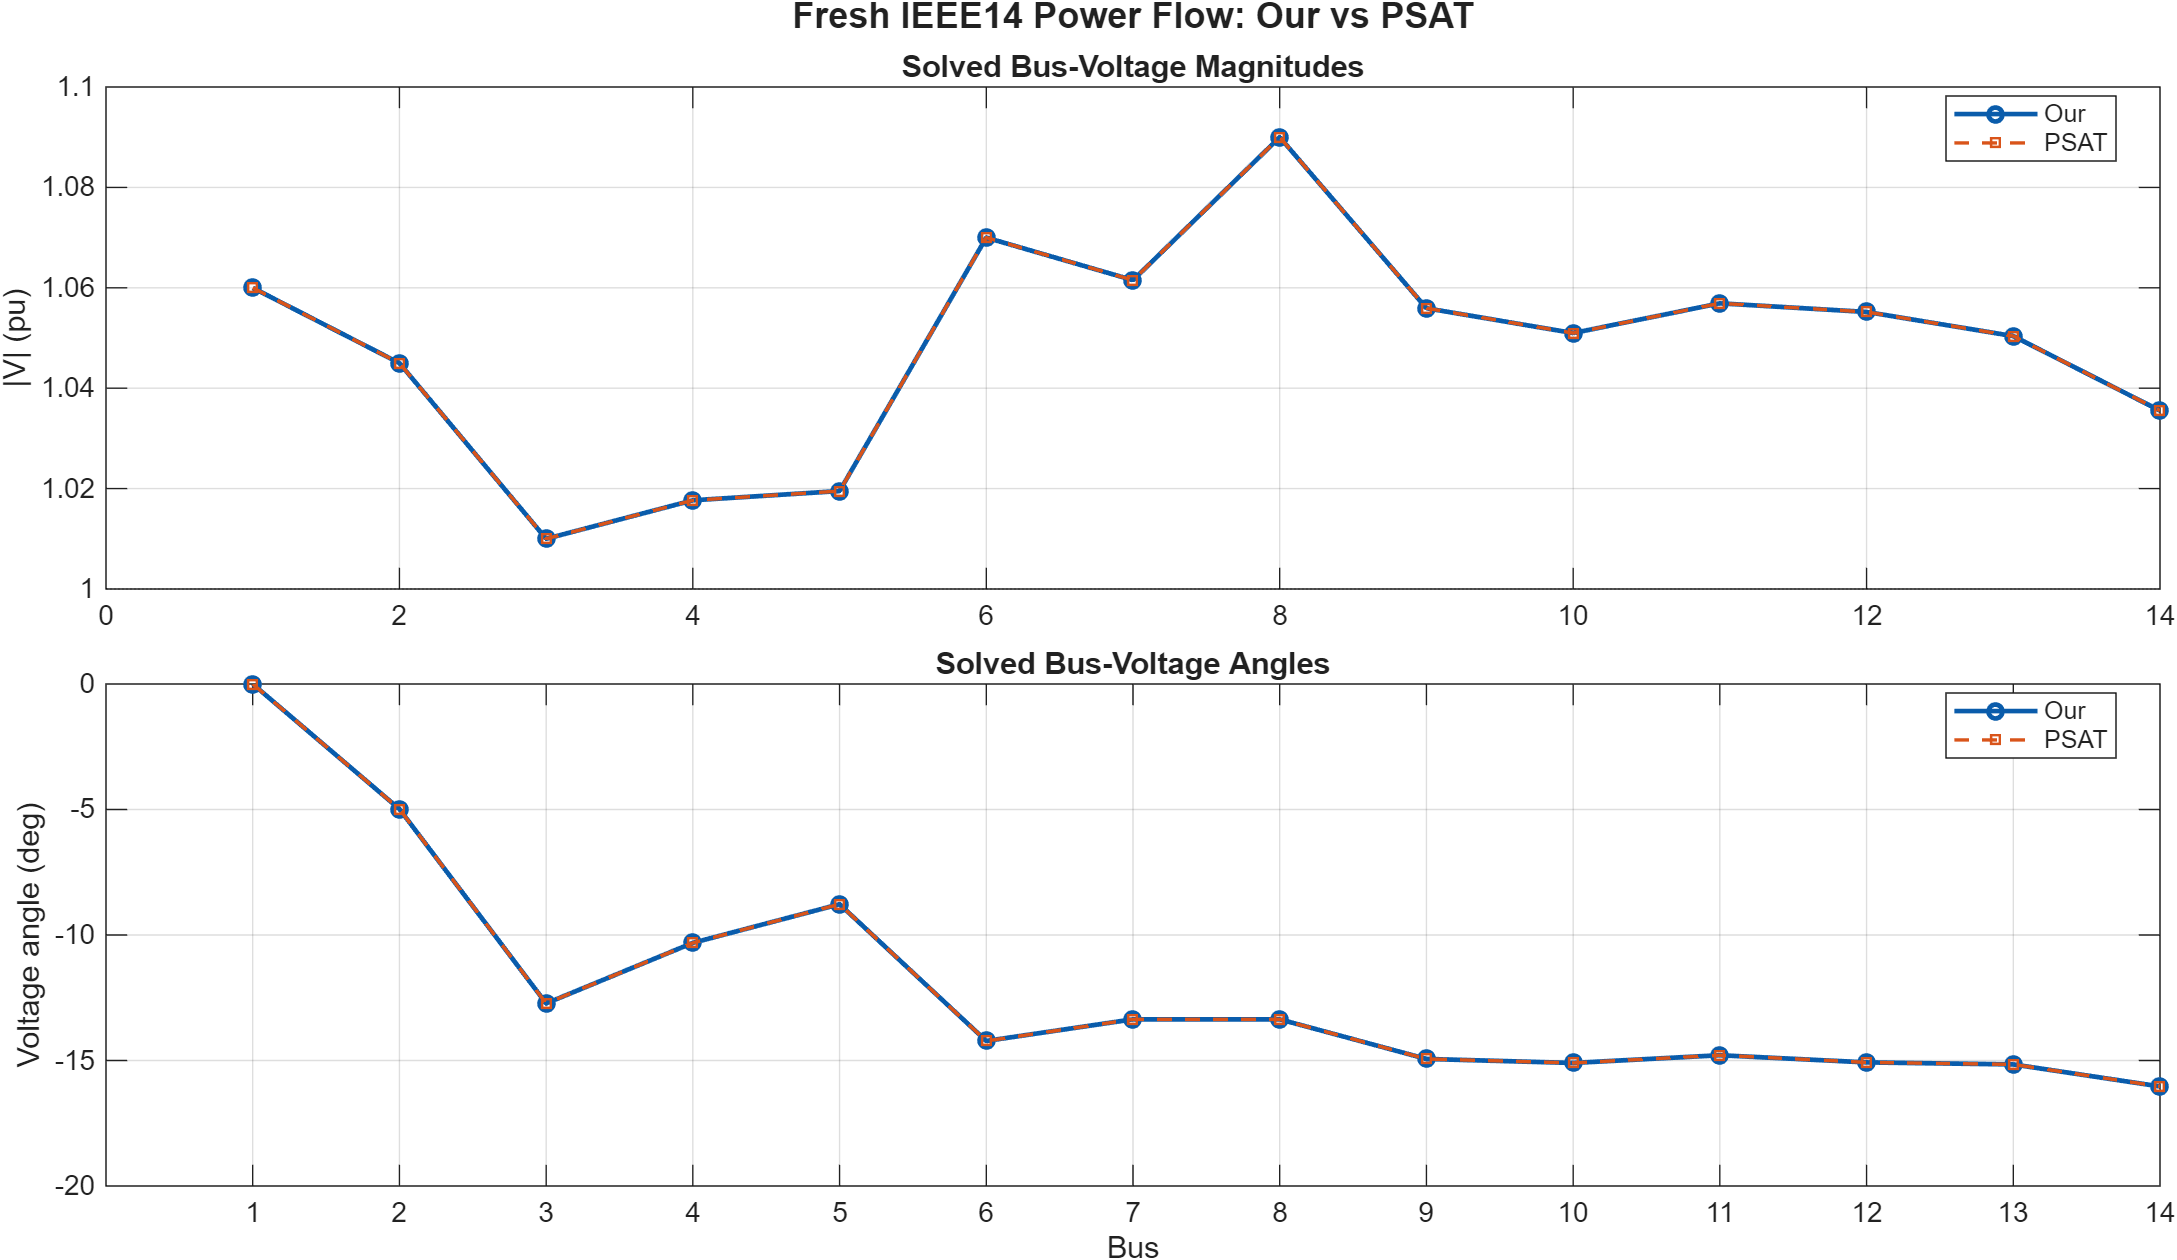
\includegraphics[width=.94\textwidth]{figures/padiyar_two_area/ieee14_pf_ours_psat.png}
\caption{Fresh IEEE14 solved bus-voltage magnitudes and angles. Our is solid
and PSAT is dashed; both traces use the bus-ID mapping reported in
Table~\ref{tab:ieee14-pf}.}
\label{fig:ieee14-pf-solution}
\end{figure}

\begin{figure}[H]\centering
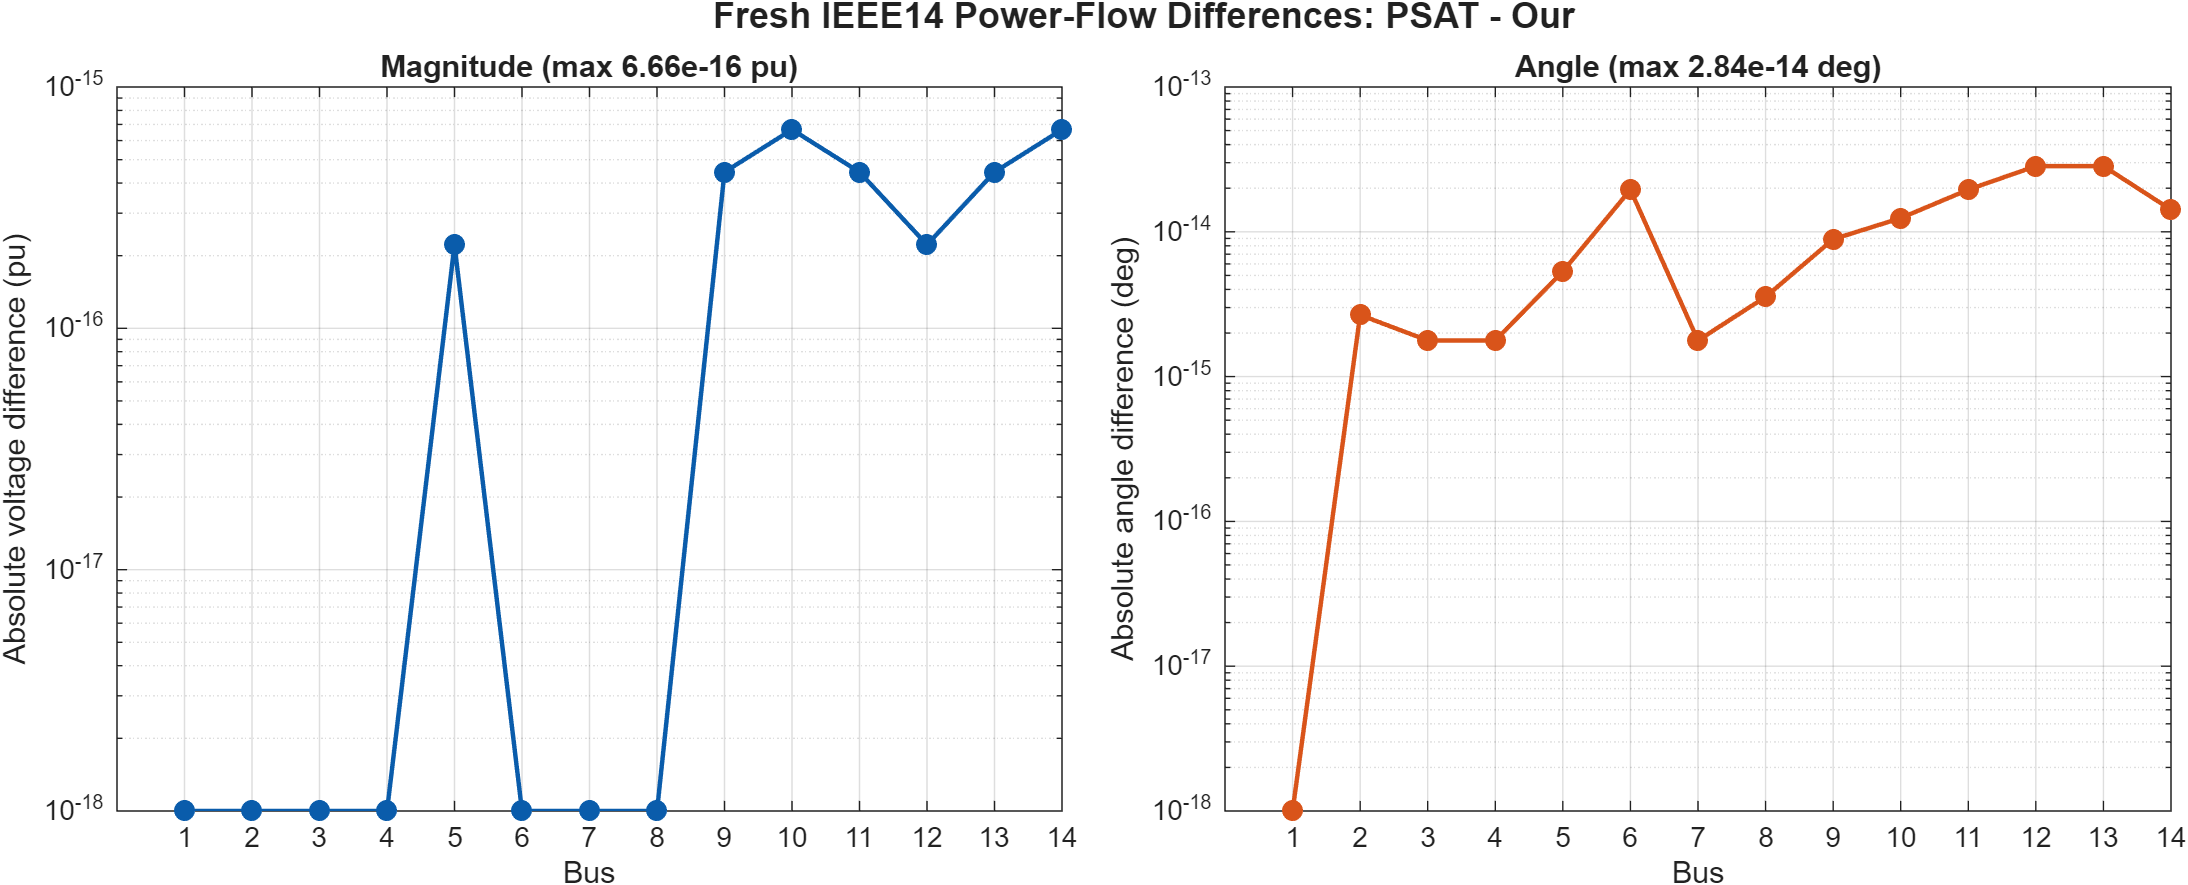
\includegraphics[width=.94\textwidth]{figures/padiyar_two_area/ieee14_pf_error_ours_psat.png}
\caption{Per-bus absolute PF differences from the same fresh Our and PSAT
solutions. Zero differences are shown at the numerical display floor on the
logarithmic axes.}
\label{fig:ieee14-pf-error}
\end{figure}

\subsection{Small-signal stability results}

Table~\ref{tab:ieee14-sssa} compares the positive-imaginary physical relative
modes from the identical five-machine classical model. The common-angle zero
mode is omitted by the declared $10^{-3}$~rad/s frequency threshold. PSAT
values are reported exactly as returned by its state-matrix analysis; its
\path{fm_eigen} implementation applies a documented $-10^{-6}$ diagonal
shift. No equation is repeated here because the model and linearisation have
already been described above.

\begin{table}[H]\centering\small
\caption{Fresh IEEE14 SSSA modal comparison: Our versus raw PSAT output.}
\label{tab:ieee14-sssa}
\resizebox{\textwidth}{!}{% Fresh Our and raw PSAT SSSA modes; common-angle zero modes excluded a priori.
\begin{tabular}{r cc r rr rr}\toprule
Mode & {$\lambda_{Our}$} & {$\lambda_{PSAT}$} & {$|\Delta\lambda|$} & {$f_{Our}$} & {$f_{PSAT}$} & {$\zeta_{Our}$} & {$\zeta_{PSAT}$} \\ 
{} & {(s$^{-1}$)} & {(s$^{-1}$)} & {(s$^{-1}$)} & {(Hz)} & {(Hz)} & {(\%)} & {(\%)} \\ \midrule
1 & {$-0.000000+11.520207j$} & {$-0.000001+11.520207j$} & 1.000e-06 & 1.83350 & 1.83350 & 0.00000 & 0.00001 \\
2 & {$0.000000+9.955055j$} & {$-0.000001+9.955055j$} & 1.000e-06 & 1.58440 & 1.58440 & -0.00000 & 0.00001 \\
3 & {$-0.000000+9.621911j$} & {$-0.000001+9.621911j$} & 1.000e-06 & 1.53137 & 1.53137 & 0.00000 & 0.00001 \\
4 & {$0.000000+8.505808j$} & {$-0.000001+8.505808j$} & 1.000e-06 & 1.35374 & 1.35374 & -0.00000 & 0.00001 \\
\bottomrule\end{tabular}
}
\end{table}

\begin{figure}[H]\centering
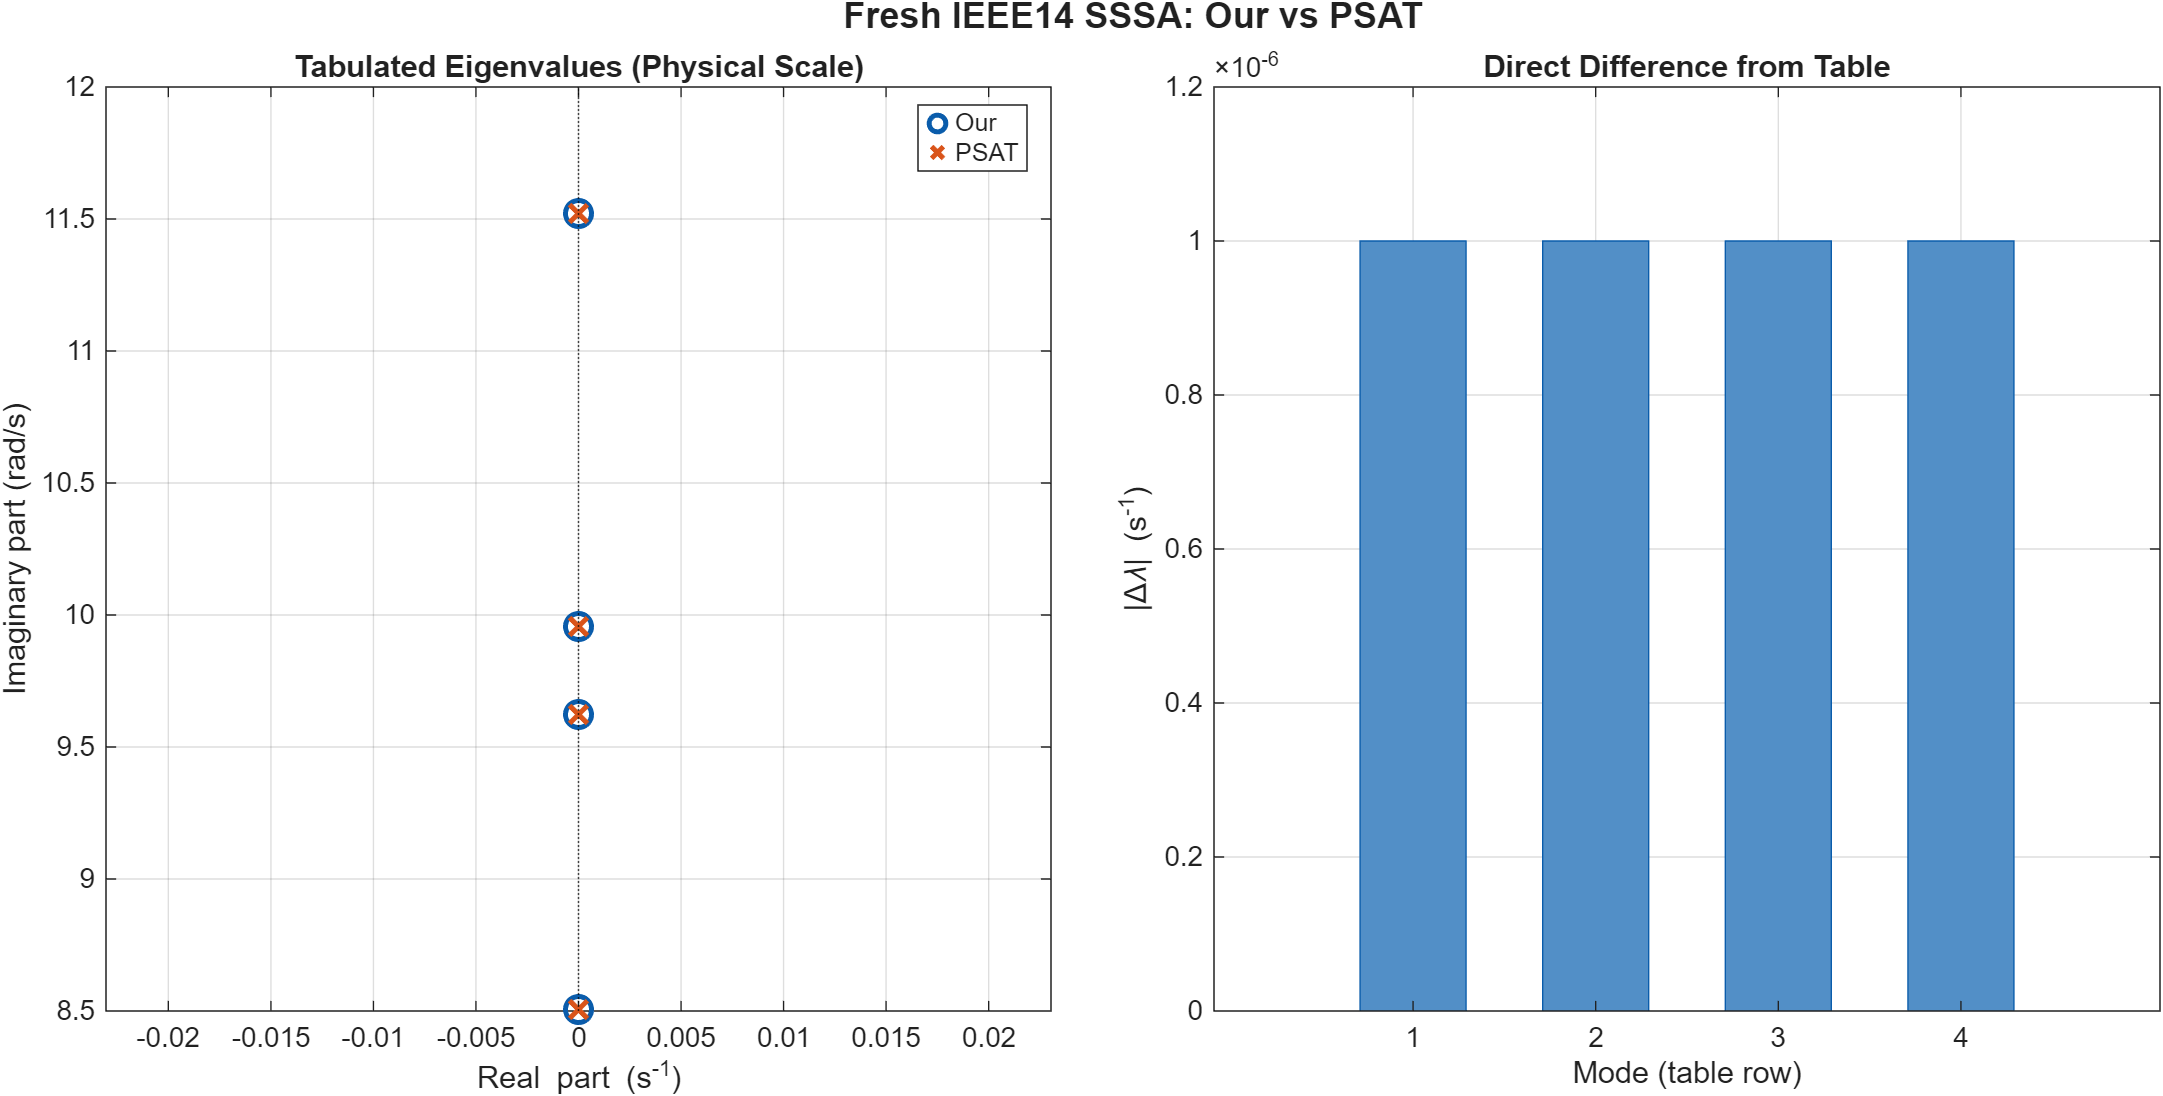
\includegraphics[width=.91\textwidth]{figures/padiyar_two_area/ieee14_sssa_complex_ours_psat.png}
\caption{Fresh IEEE14 positive-imaginary modes plotted directly from
Table~\ref{tab:ieee14-sssa}. The complex-plane panel uses the unscaled
eigenvalues in physical units; the difference panel reports the corresponding
$|\Delta\lambda|$ for each table row.}
\label{fig:ieee14-sssa-complex}
\end{figure}

\begin{figure}[H]\centering
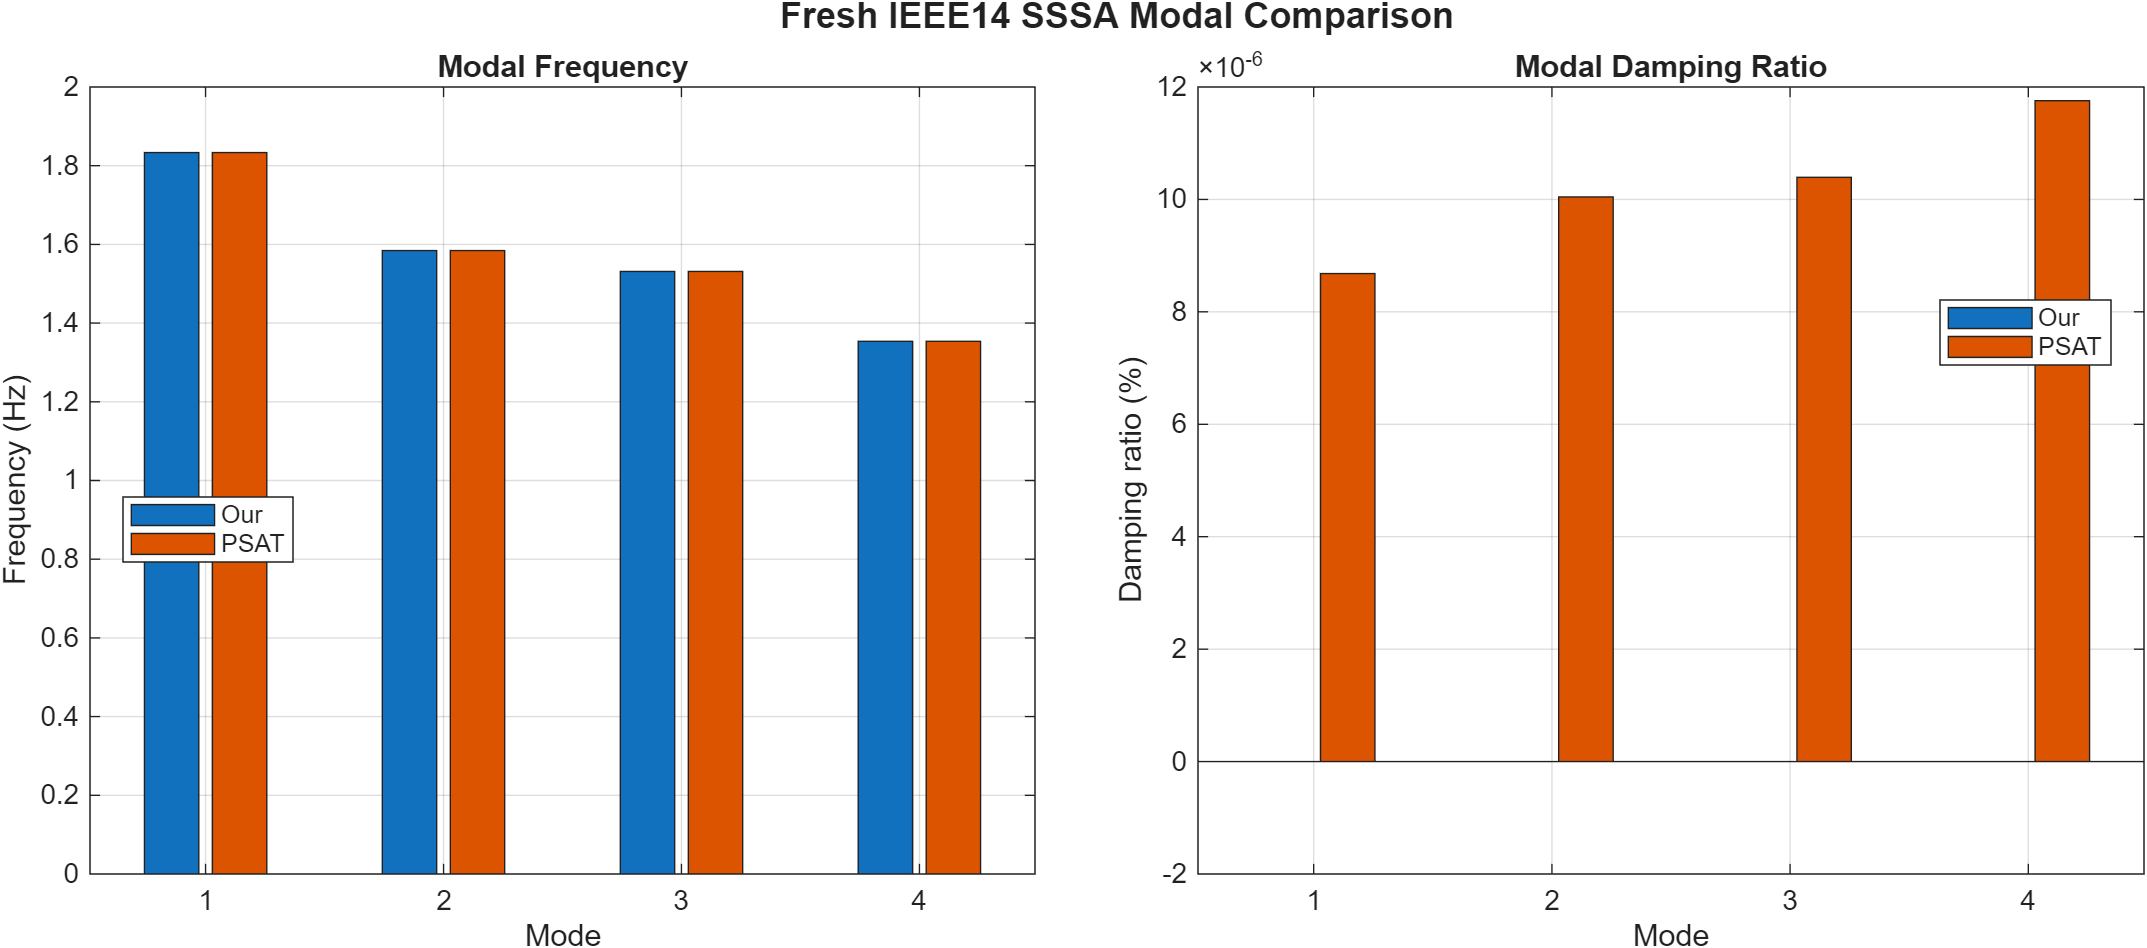
\includegraphics[width=.94\textwidth]{figures/padiyar_two_area/ieee14_sssa_modes_ours_psat.png}
\caption{Fresh IEEE14 modal frequencies and damping ratios corresponding
directly to Table~\ref{tab:ieee14-sssa}.}
\label{fig:ieee14-sssa-modes}
\end{figure}

\subsection{Time-domain-simulation results}

Generator columns are mapped by bus ID and direct trajectory differences are
evaluated on the in-house event grid. The in-house run follows the same
\path{solve_case('analysis','ts')} execution path and MATPOWER14 defaults used
by \path{run_ts.m}. PSAT's additional internal event samples are retained in
its raw count; interpolation to the comparison grid refuses extrapolation.
Table~\ref{tab:ieee14-ts} reports each tool's response summary and the direct
PSAT--Our differences. All four figures plot the stored solver outputs:
$\delta_i(t)$, $\omega_i(t)$, $P_{e,i}(t)$ and bus-voltage magnitude. No COI,
reference-machine, initial-angle or speed-deviation transform is applied.
In every figure the upper panel overlays Our as continuous lines and PSAT as
cross markers sampled from the same comparison grid, making coincident
trajectories visible. The lower panel plots the direct PSAT--Our difference.

\begin{table}[H]\centering\small
\caption{Fresh IEEE14 TDS comparison for the bus-4, $Z_f=j10^{-4}$~pu fault.}
\label{tab:ieee14-ts}
\resizebox{\textwidth}{!}{% Fresh Our and PSAT TS results on the declared scenario.
\begin{tabular}{llrr}\toprule
Metric & Unit & Our & PSAT \\ \midrule
Completed to 15 s & -- & Yes & Yes \\
Raw time points & points & 1501 & 1509 \\
Non-converged steps & steps & 0 & {Not exposed} \\
Minimum fault-bus voltage & pu & 0.000973 & 0.000973 \\
Maximum stored rotor-angle magnitude & deg & 4964.684009 & 4964.511399 \\
Maximum stored rotor-speed magnitude & pu & 1.040163906 & 1.040155053 \\
Maximum absolute electrical power & MW & 300.383981 & 300.376323 \\ \midrule
Maximum PSAT--Our rotor-angle difference & deg & {Reference} & 1.863392e-01 \\
Maximum PSAT--Our rotor-speed difference & pu & {Reference} & 9.867292e-06 \\
Maximum PSAT--Our electrical-power difference & MW & {Reference} & 1.225034e-01 \\
Maximum PSAT--Our bus-4 voltage difference & pu & {Reference} & 7.810489e-05 \\
\bottomrule\end{tabular}
}
\end{table}

\begin{figure}[H]\centering
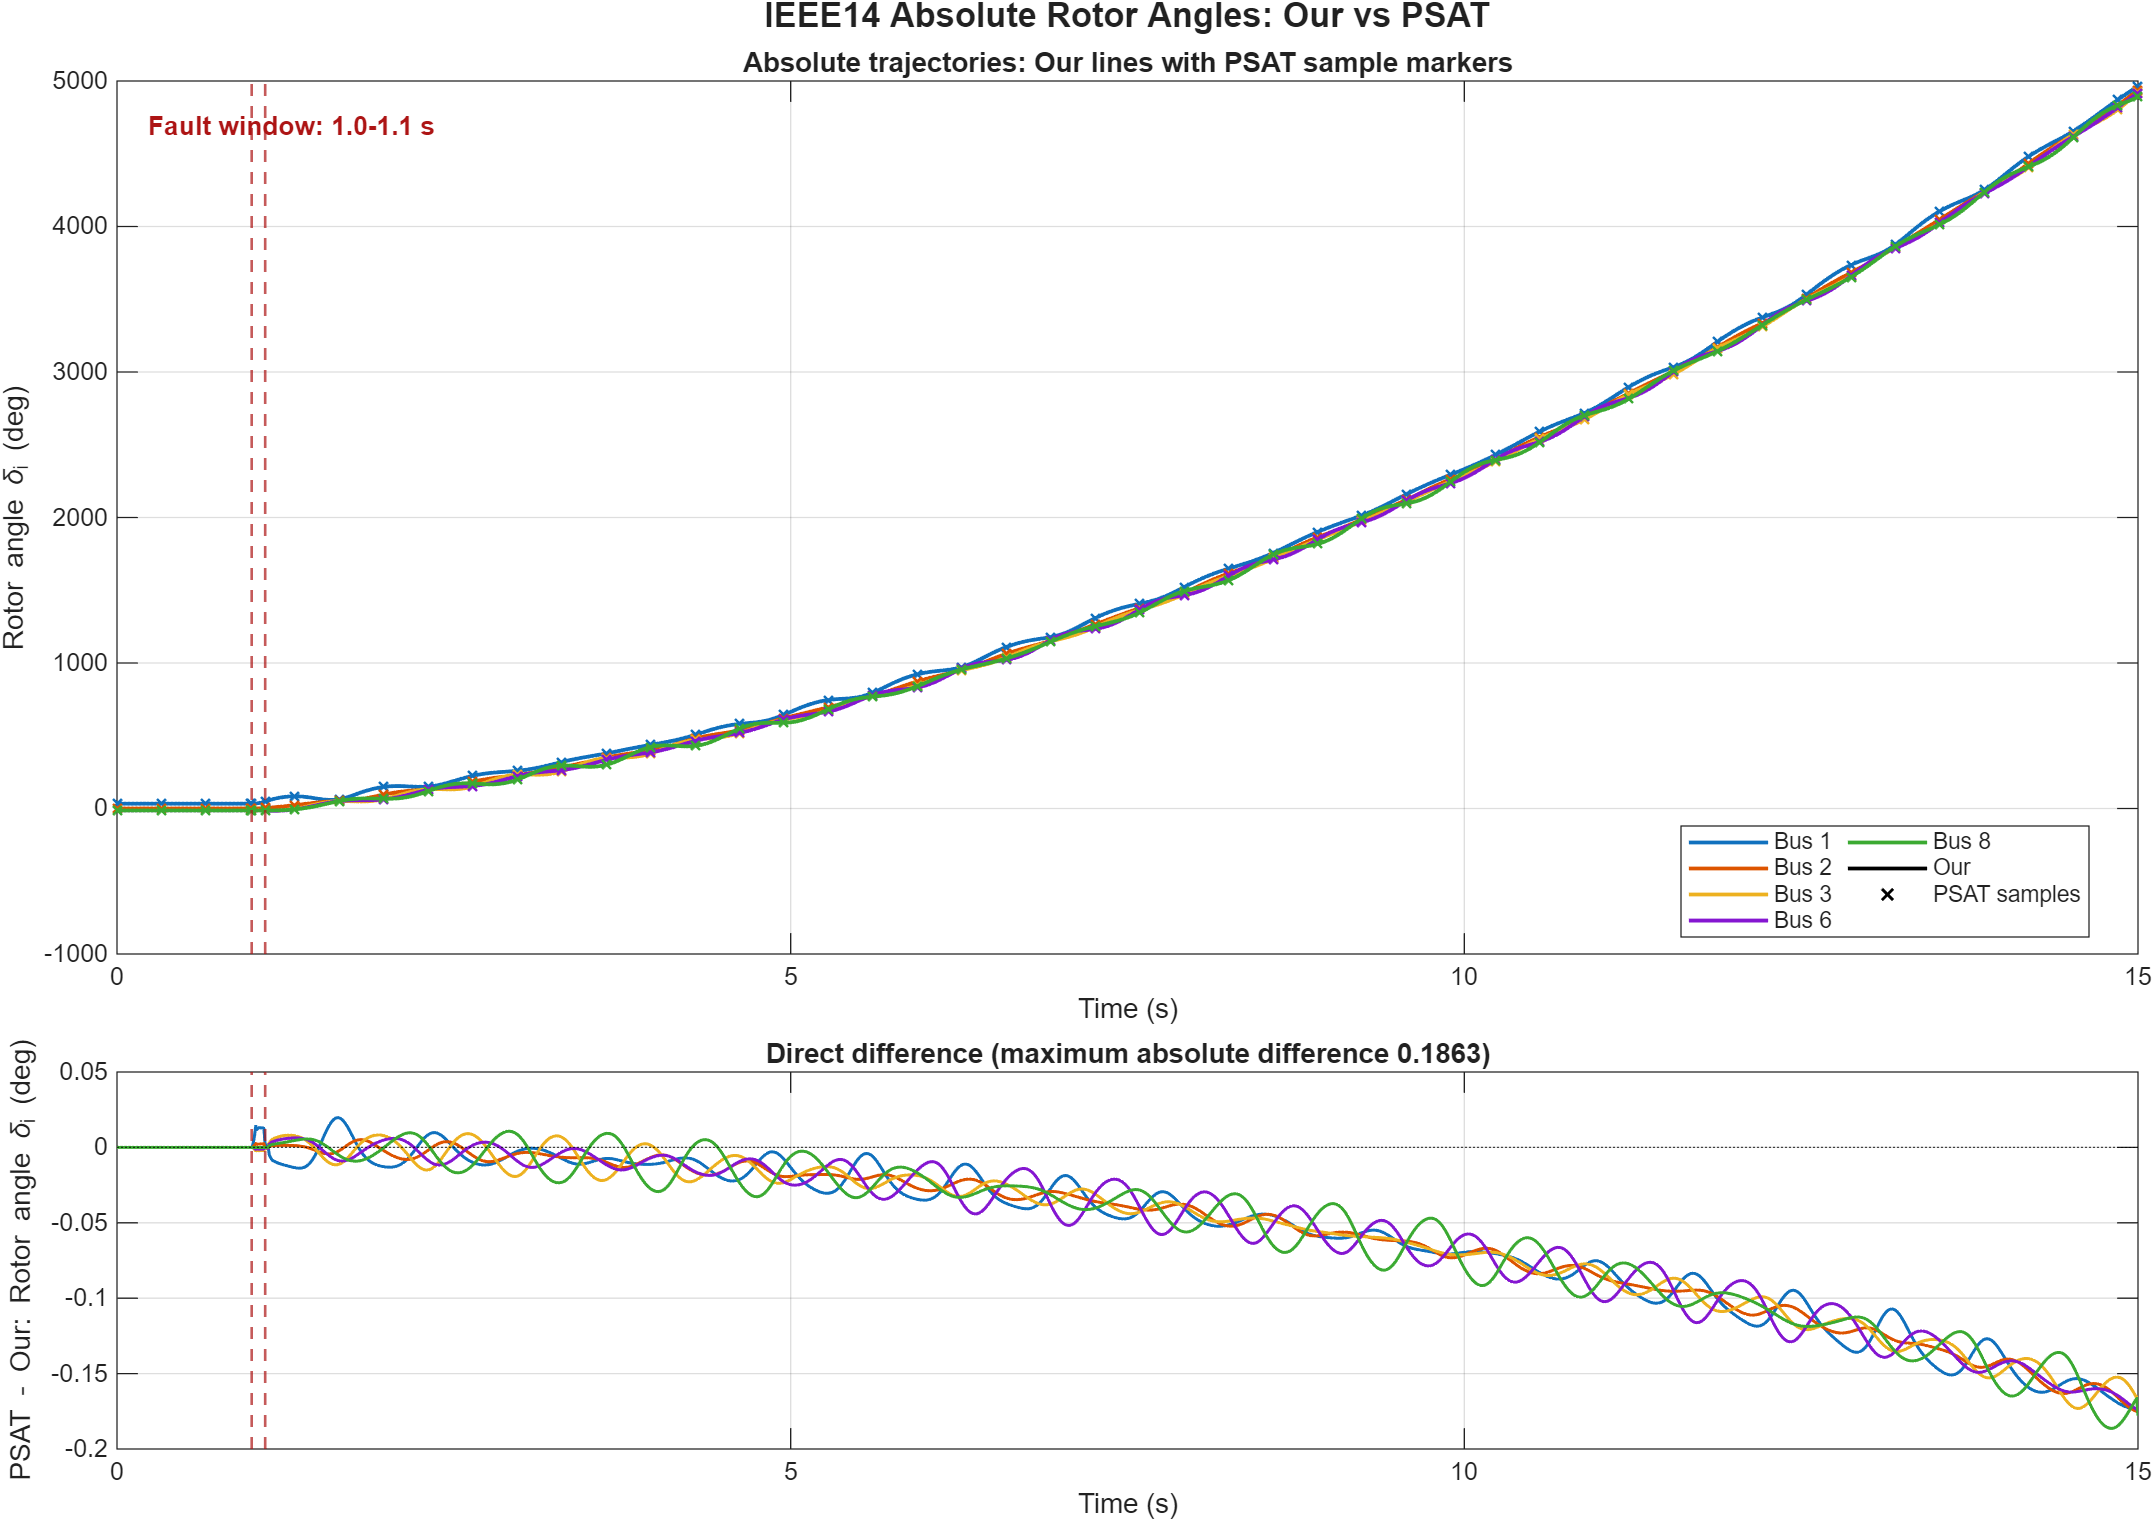
\includegraphics[width=.92\textwidth]{figures/padiyar_two_area/ieee14_ts_angle_ours_psat.png}
\caption{Fresh IEEE14 stored absolute rotor angles $\delta_i(t)$ for the five
generator buses, using the \texttt{run\_ts.m} plotting convention. No COI,
reference-machine or initial-angle subtraction is applied. Colours identify
buses. Upper panel: Our lines and PSAT cross markers. Lower panel: direct
PSAT--Our angle differences.}
\label{fig:ieee14-ts-angle}
\end{figure}

\begin{figure}[H]\centering
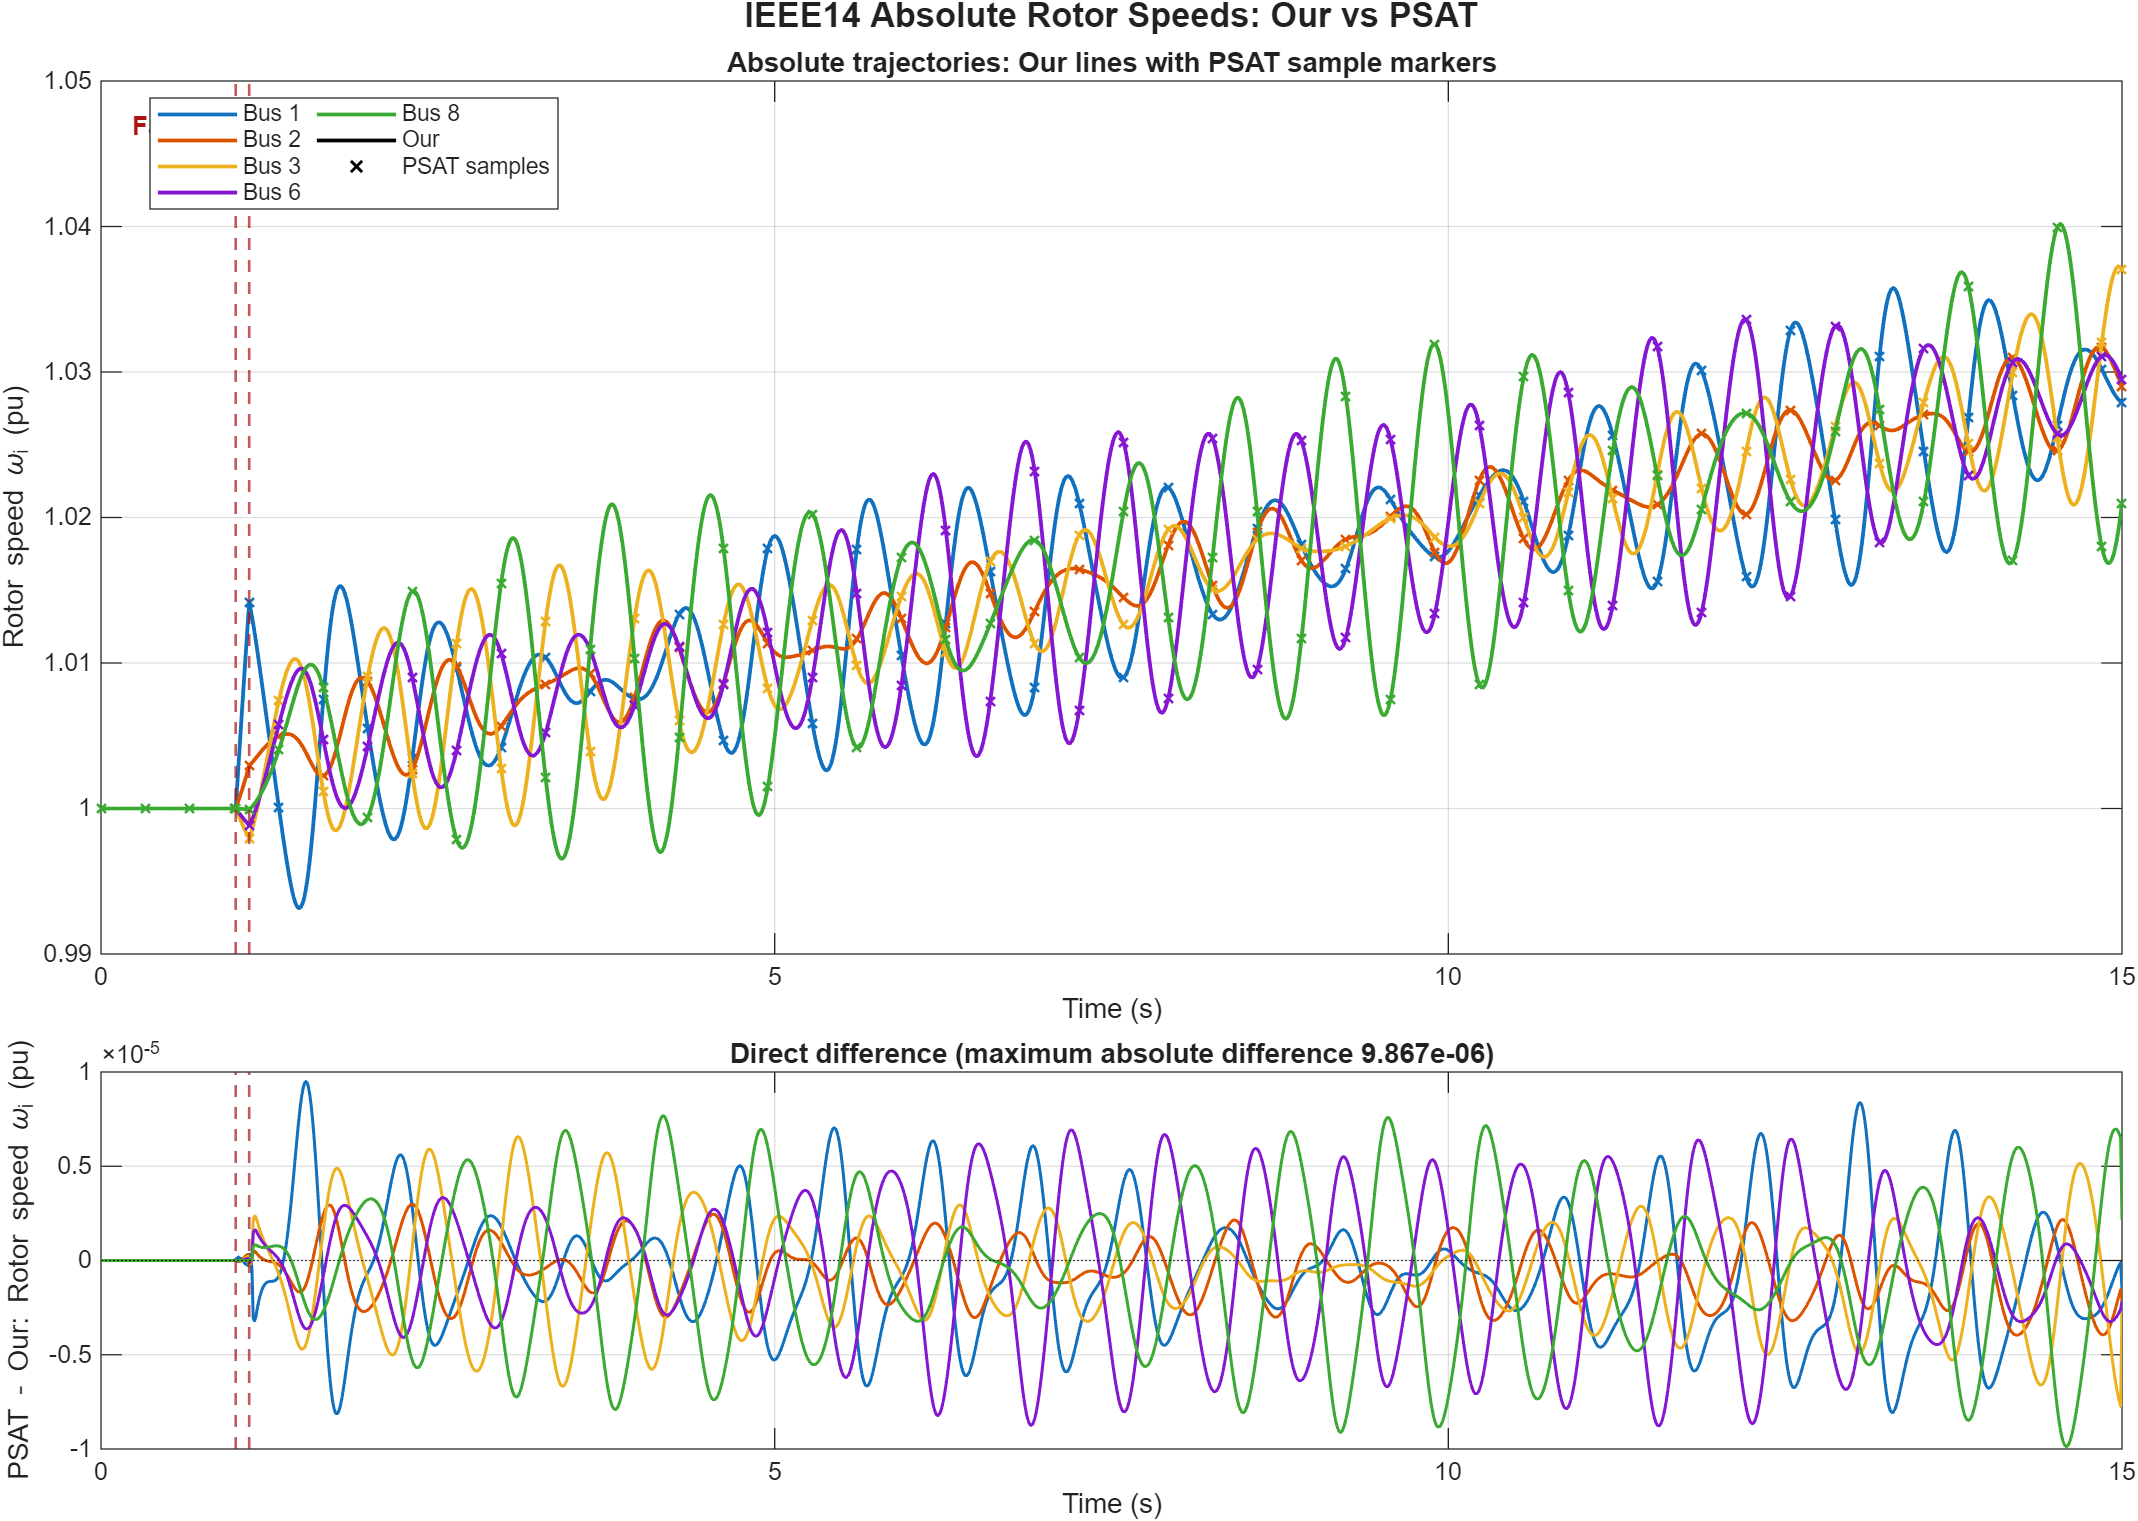
\includegraphics[width=.92\textwidth]{figures/padiyar_two_area/ieee14_ts_omega_ours_psat.png}
\caption{Fresh IEEE14 stored absolute rotor speeds $\omega_i(t)$ in per unit,
using the \texttt{run\_ts.m} plotting convention. No COI subtraction and no
$\omega_i-1$ transform is applied. Upper panel: Our lines and PSAT cross
markers. Lower panel: direct PSAT--Our speed differences.}
\label{fig:ieee14-ts-omega}
\end{figure}

\begin{figure}[H]\centering
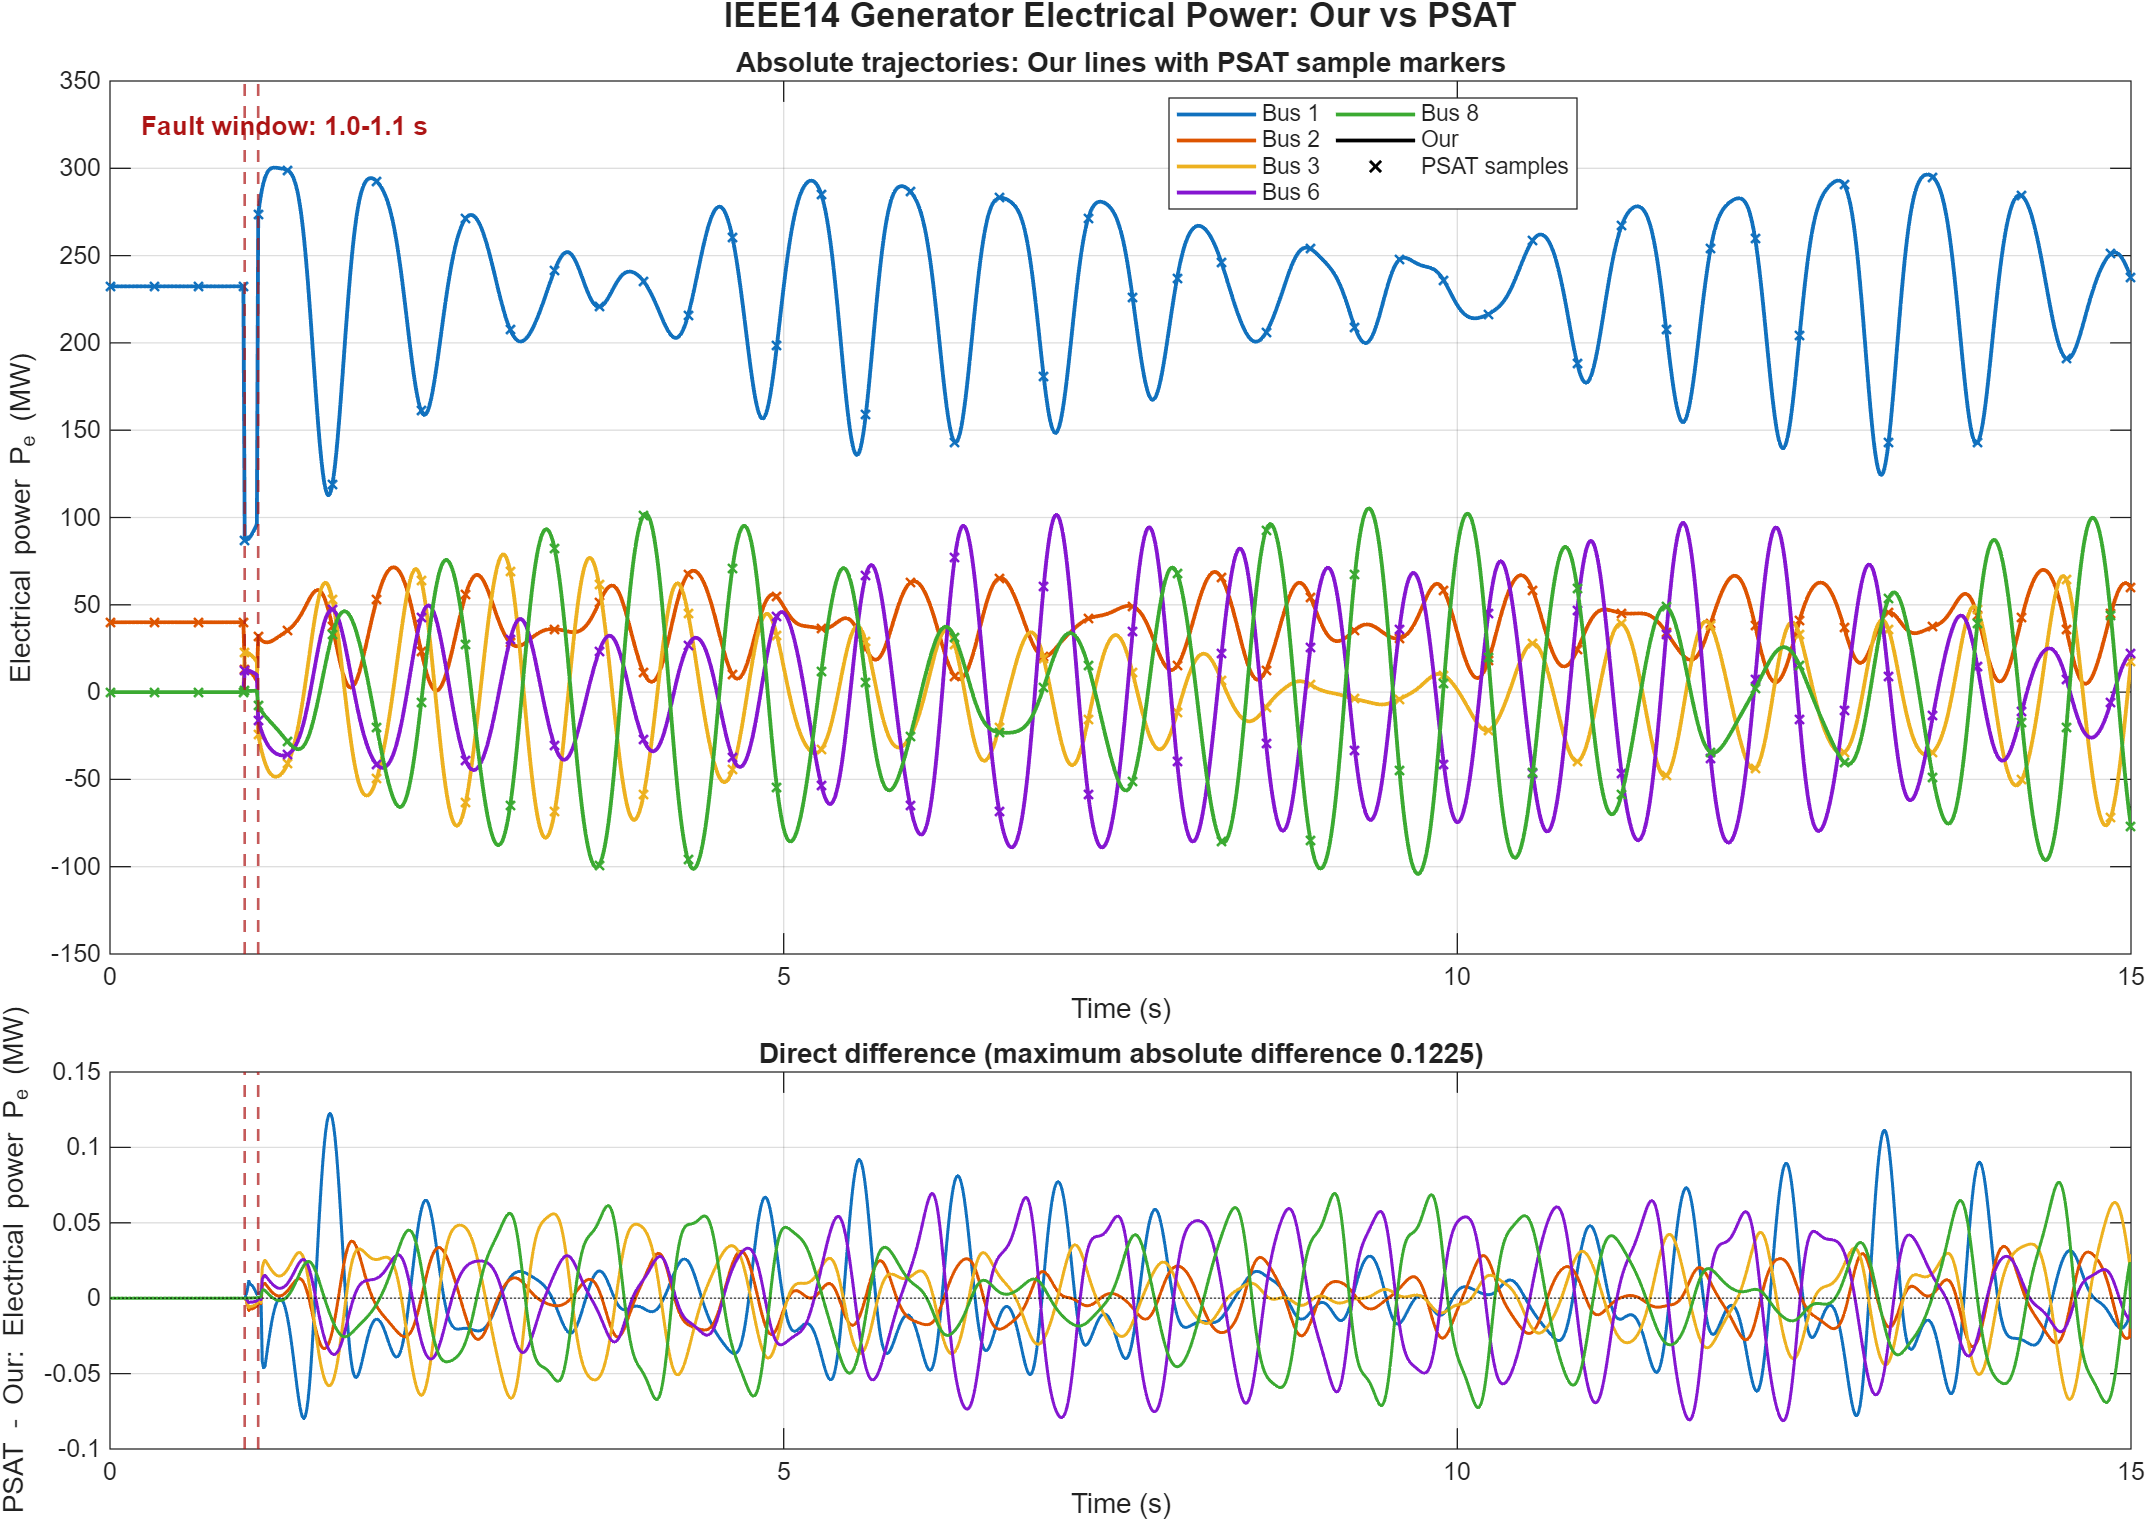
\includegraphics[width=.92\textwidth]{figures/padiyar_two_area/ieee14_ts_pe_ours_psat.png}
\caption{Fresh IEEE14 stored generator electrical powers $P_{e,i}(t)$, using
the \texttt{run\_ts.m} plotting convention. Upper panel: Our lines and PSAT
cross markers. Lower panel: direct PSAT--Our electrical-power differences.}
\label{fig:ieee14-ts-pe}
\end{figure}

\begin{figure}[H]\centering
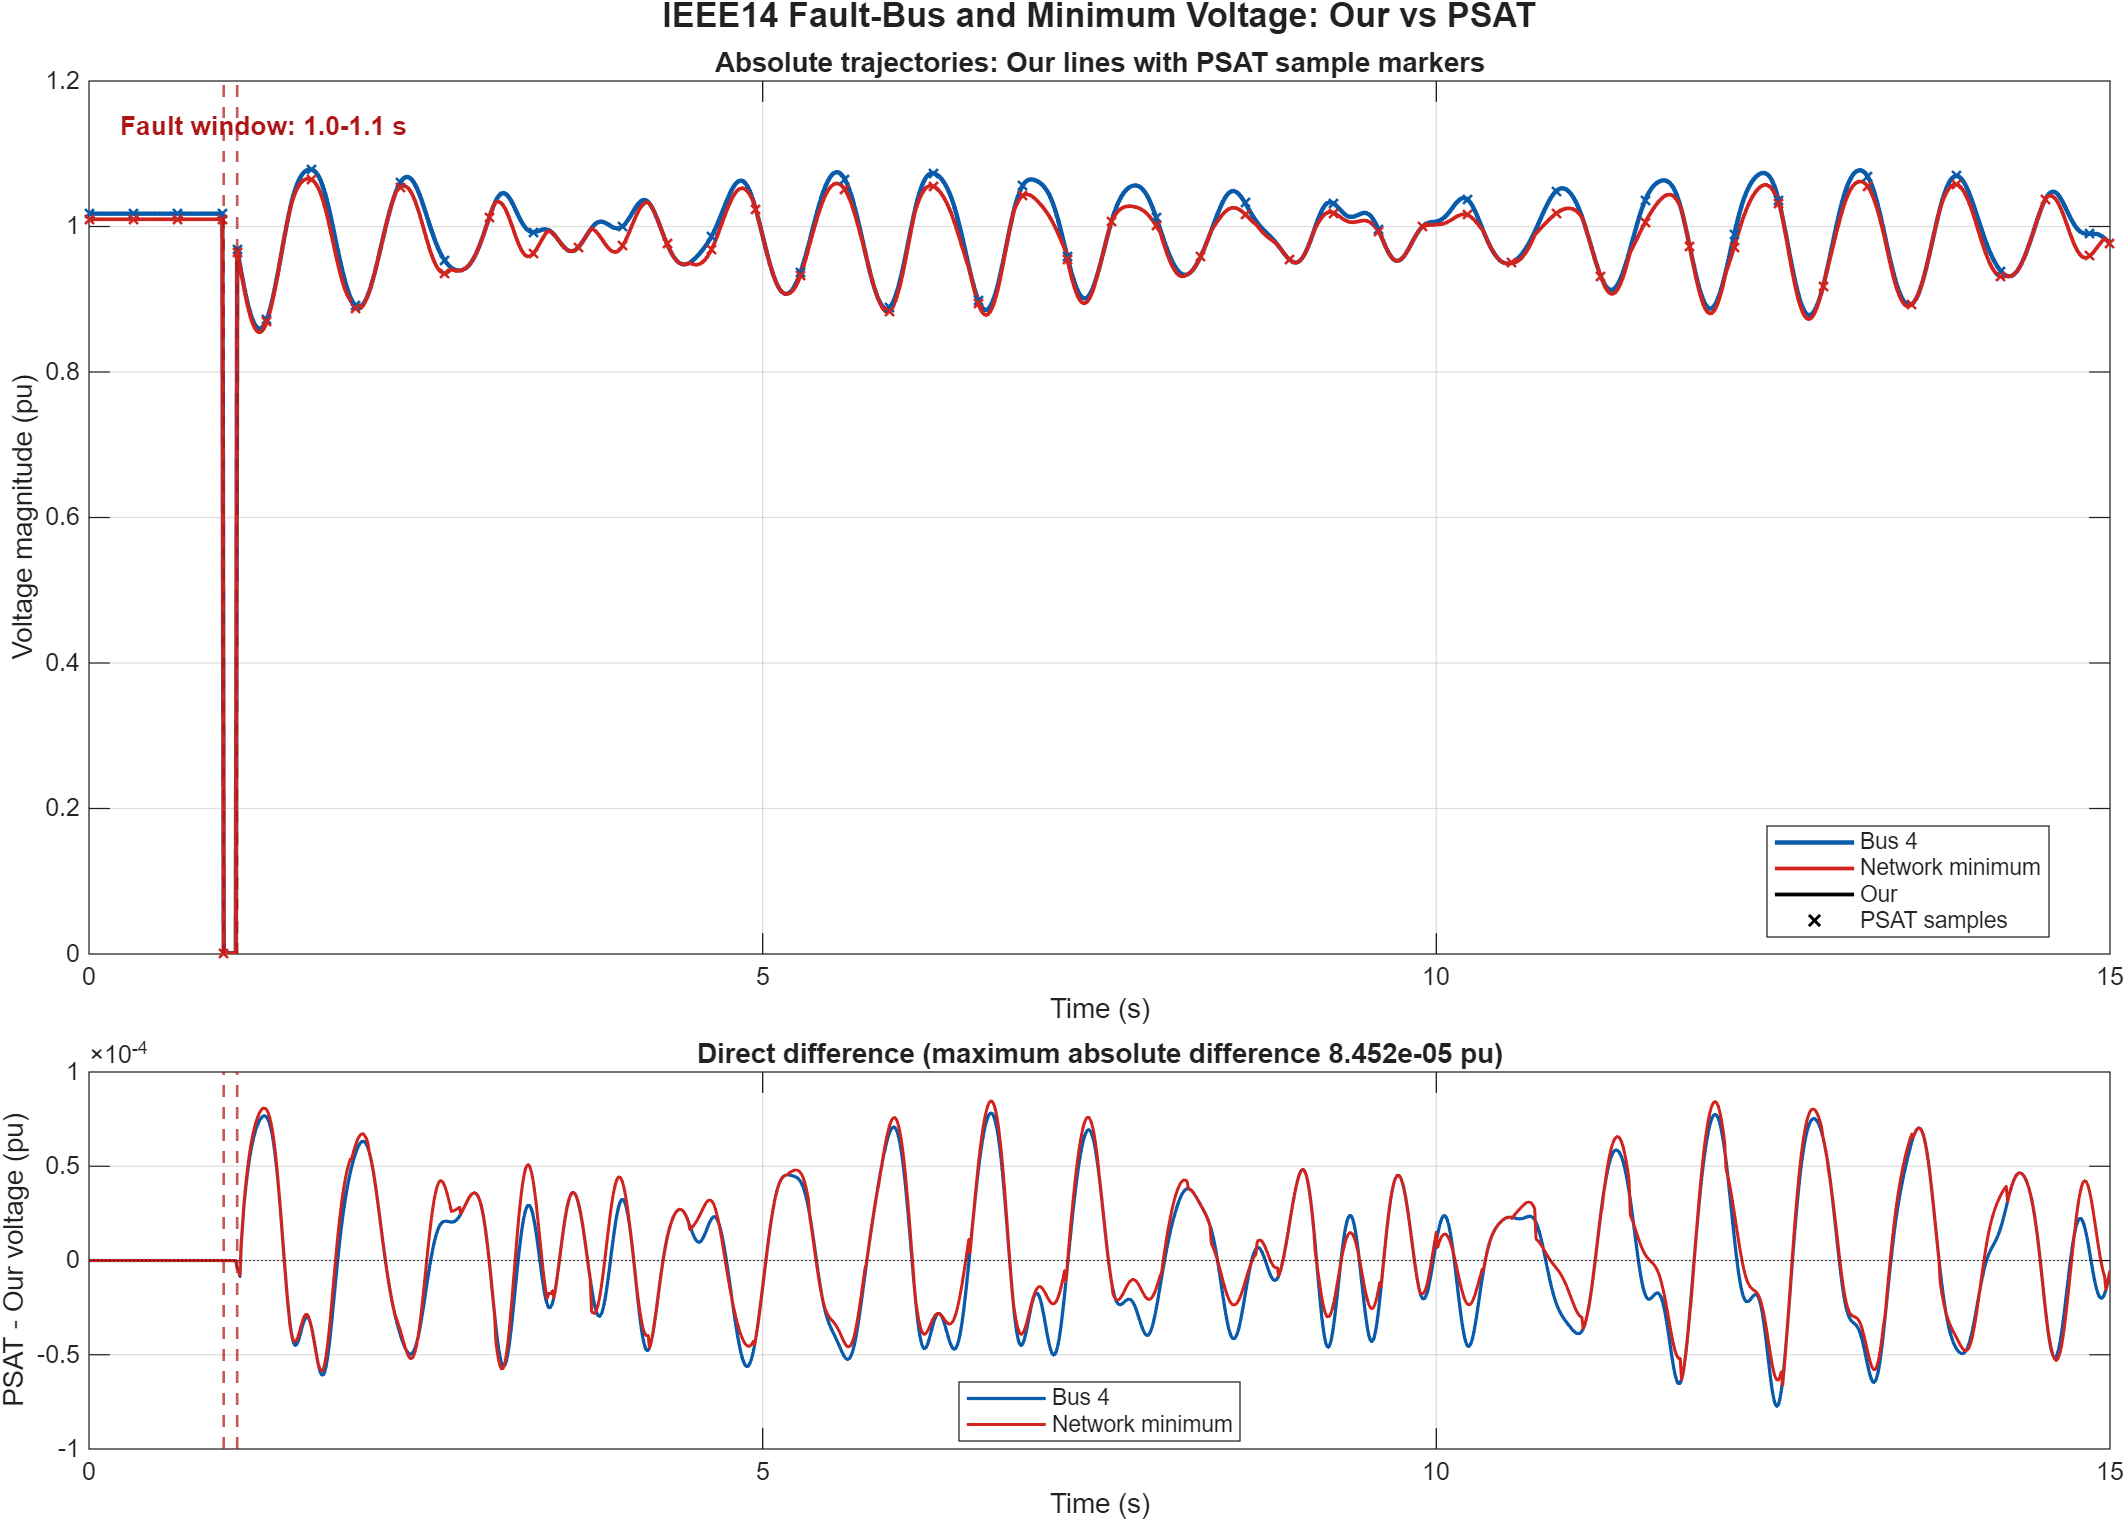
\includegraphics[width=.92\textwidth]{figures/padiyar_two_area/ieee14_ts_voltage_ours_psat.png}
\caption{Fresh IEEE14 bus-4 and minimum-network voltage magnitudes for the
declared fault, using the \texttt{run\_ts.m} plotting convention. Upper panel:
Our lines and PSAT cross markers. Lower panel: direct PSAT--Our voltage
differences.}
\label{fig:ieee14-ts-voltage}
\end{figure}

\section{Conclusions}

The Padiyar two-area case provides a traceable replacement reference for the
project. It reproduces Table~9.2 with the in-house power flow, implements the
source's actual five-state AVR model, exposes a manual-excitation comparison,
and runs SSSA and residual-checked TS from one DAE. No subtransient parameter or
PSS setting is fabricated. The next extension may add a documented PSS design
and then use this frozen SG baseline for SG-to-VSG replacement studies.

\end{document}
